% Template for a Computer Science Tripos Part II project dissertation
\documentclass[12pt,a4paper,twoside,openright]{report}
\usepackage[pdfborder={0 0 0}, colorlinks=true, linkcolor=black, citecolor=black, filecolor=magenta, urlcolor=cyan]{hyperref}    % turns references into hyperlinks
\usepackage[margin=25mm]{geometry}  % adjusts page layout
\usepackage{graphicx}  % allows inclusion of PDF, PNG and JPG images
\usepackage{verbatim}
\usepackage{docmute}   % only needed to allow inclusion of proposal.tex

% custom headers by pv273
\usepackage[ampersand]{easylist}
\usepackage{algorithm}
\usepackage{algpseudocode}
\usepackage{amsbsy}
\usepackage{amsfonts}
\usepackage{amsmath}
\usepackage{amssymb}
\usepackage{amsthm}
\usepackage{booktabs}
\usepackage{caption}
\usepackage{color} 
\usepackage{cleveref}
\usepackage{empheq}
\usepackage{enumitem}
\usepackage{etex}
\usepackage{fancyhdr}
\usepackage{float}
\usepackage{footnote}
\usepackage{framed}
\usepackage[T1]{fontenc}
\usepackage[UKenglish]{isodate}
\usepackage{latexsym}
\usepackage{leftidx}
\usepackage{listings}
\usepackage{mathrsfs}
\usepackage{mathtools}
\usepackage{multicol}
\usepackage{pgfplots}
\usepackage{soul}
\usepackage{subfig}
\usepackage{tikz}
\usepackage[nottoc]{tocbibind}

\cleanlookdateon

\font \cyr=wncyr10 at 12pt
\font \cyi=wncyi10 at 12pt

\definecolor{echoreg}{HTML}{2cb1e1}
\definecolor{echodrk}{HTML}{0099cc}
\definecolor{echobg}{HTML}{eaeaea}
\definecolor{sublimedg}{HTML}{171813}
\definecolor{sublimelg}{HTML}{272822}
\definecolor{olivegreen}{rgb}{0,0.6,0}
\definecolor{myorange}{rgb}{1,0.25,0}
\definecolor{drkorange}{HTML}{FF7c00}

\DeclareCaptionFormat{listing}{#1#2#3}

\renewcommand{\algorithmicrequire}{\textbf{Input:}}
\renewcommand{\algorithmicensure}{\textbf{Output:}}

% setting up libraries, by pv273

\crefname{section}{\S\!\!}{\S}
\Crefname{section}{\S\!\!}{\S}

\setcounter{tocdepth}{3}
\setcounter{secnumdepth}{3}

\newtheorem{mydef}{Definition}
\newcommand\myeq{\stackrel{\mathclap{\tiny\mbox{def}}}{=}}
\newcommand\Prob{\mathbb{P}}
\newcommand\Like{\mathbb{L}}
\newcommand{\argmax}{\operatornamewithlimits{argmax}}
\newcommand\bomega{\boldsymbol\omega}

% CPP LOGO
\def\CC{{C\nolinebreak[4]\hspace{-.05em}\raisebox{.4ex}{\tiny\bf ++}}}

%% TikZ
\usetikzlibrary{arrows,decorations.pathmorphing,backgrounds,positioning,fit,petri}
\usetikzlibrary{shapes.geometric, automata, chains}

\tikzset{
    triangle/.style={
        draw,
        shape border rotate=0,
        regular polygon,
        regular polygon sides=3,
        fill=white,
        node distance=2cm,
        minimum height=4em,
        minimum size=4mm,
        inner sep=0pt
    }
}
\tikzstyle{decision} = [diamond, draw, fill=blue!20, 
    text width=4.5em, text badly centered, node distance=3cm, inner sep=0pt]
\tikzstyle{block} = [rectangle, draw, fill=blue!20, 
    text width=7em, text centered, rounded corners, minimum height=4em]
\tikzstyle{line} = [draw, -stealth, very thick]
\tikzstyle{cloud} = [draw, ellipse,fill=red!20, node distance=3cm,
    minimum height=2em]
    
\tikzstyle{block2} = [rectangle, draw, fill=blue!20, 
    text width=4em, text centered, rounded corners, minimum height=1em]

%% Custom colours
\definecolor{darkgreen}{rgb}{0.0, 0.42, 0.24}
\definecolor{light-gray}{gray}{0.85}
% C++ Code
\definecolor{mygreen}{rgb}{0,0.6,0}
\definecolor{mygray}{rgb}{0.5,0.5,0.5}
\definecolor{mymauve}{rgb}{0.58,0,0.82}

\newcommand\mycirc{\tikz\node[circle, minimum size=.4cm,fill=red]{};}
\newcommand\myrect{\tikz\node[rectangle, minimum size=.4cm, fill=echodrk]{};}

\newcommand{\mytilde}{\raise.17ex\hbox{$\scriptstyle\mathtt{\sim}$}}

%% code listing
\lstset{ %
  backgroundcolor=\color{white},   % choose the background color; you must add \usepackage{color} or \usepackage{xcolor}
  basicstyle=\footnotesize\ttfamily,        % the size of the fonts that are used for the code
  %belowskip=-0.8\baselineskip,
  breakatwhitespace=false,         % sets if automatic breaks should only happen at whitespace
  breaklines=true,                 % sets automatic line breaking
  captionpos=b,                    % sets the caption-position to bottom
  commentstyle=\color{mygreen},    % comment style
  deletekeywords={...},            % if you want to delete keywords from the given language
  escapeinside={\%*}{*)},          % if you want to add LaTeX within your code
  extendedchars=true,              % lets you use non-ASCII characters; for 8-bits encodings only, does not work with UTF-8
  frame=false,                    % adds a frame around the code
  keepspaces=true,                 % keeps spaces in text, useful for keeping indentation of code (possibly needs columns=flexible)
  keywordstyle=\color{blue},       % keyword style
  language=C++,                 % the language of the code
  literate={~} {\mytilde}{1},
  morekeywords={*,...},            % if you want to add more keywords to the set
  numbers=left,                    % where to put the line-numbers; possible values are (none, left, right)
  numbersep=5pt,                   % how far the line-numbers are from the code
  numberstyle=\tiny\color{mygray}, % the style that is used for the line-numbers
  rulecolor=\color{black},         % if not set, the frame-color may be changed on line-breaks within not-black text (e.g. comments (green here))
  showspaces=false,                % show spaces everywhere adding particular underscores; it overrides 'showstringspaces'
  showstringspaces=false,          % underline spaces within strings only
  showtabs=false,                  % show tabs within strings adding particular underscores
  stepnumber=1,                    % the step between two line-numbers. If it's 1, each line will be numbered
  stringstyle=\color{mymauve},     % string literal style
  tabsize=2,                       % sets default tabsize to 2 spaces
  title=\lstname                   % show the filename of files included with \lstinputlisting; also try caption instead of title
}

\newcommand{\yslant}{0.5}
\newcommand{\xslant}{-0.6}

\raggedbottom                           % try to avoid widows and orphans
\sloppy
\clubpenalty1000%
\widowpenalty1000%

\renewcommand{\baselinestretch}{1.1}    % adjust line spacing to make
                                        % more readable

\begin{document}

\bibliographystyle{plain}

\newcommand{\HRule}{\rule{\linewidth}{0.5mm}} % Defines a new command for the horizontal lines, change thickness here

%%%%%%%%%%%%%%%%%%%%%%%%%%%%%%%%%%%%%%%%%%%%%%%%%%%%%%%%%%%%%%%%%%%%%%%%
% Title
%TC:ignore

\pagestyle{empty}

\rightline{\LARGE \textbf{Petar Veli\v{c}kovi\'{c}}}

\vspace*{60mm}
\begin{center}
\Huge\HRule\\[0.4cm] %0.4cm
	{\bf Molecular multiplex network inference}
	\HRule \\[20pt] %20pt
Project Dissertation \\
Computer Science Tripos, Part II \\[5mm]
Trinity College \\[5mm]
\today  % today's date
\end{center}

%%%%%%%%%%%%%%%%%%%%%%%%%%%%%%%%%%%%%%%%%%%%%%%%%%%%%%%%%%%%%%%%%%%%%%%%%%%%%%
% Proforma, table of contents and list of figures

\chapter*{Proforma}

\pagenumbering{roman}
\pagestyle{plain}
\setcounter{page}{1}

{\large
\begin{tabular}{ll}
Name:               & \bf Petar Veli\v{c}kovi\'{c}                       \\
College:            & \bf Trinity College                     \\
Project Title:      & \bf Molecular multiplex network inference \\
Examination:        & \bf Computer Science Tripos, Part II, 2015  \\
Word Count:         & \bf 11974\footnotemark  \\
Project Originators: & {\bf Dr Pietro Li\`{o}} and {\bf Petar Veli\v{c}kovi\'{c}}                    \\
Supervisor:         & \bf Dr Pietro Li\`{o}                    \\ 
\end{tabular}
}
\footnotetext{The word count has been computed by \TeX count, \url{http://app.uio.no/ifi/texcount/}.}\stepcounter{footnote}


\section*{Original Aims of the Project}

The primary aim of this project is to investigate the potentials of utilising complex networks to handle multiple types of correlated data simultaneously when making inferences in the context of binary classification problems. In order to do this, a generic machine learning library that uses multiplex networks was to be implemented and evaluated; the evaluation consists of assessing the performance benefits of this approach on synthetic and biomolecular data sets (utilising standard machine learning evaluation metrics), in particular compared to the single-layer versions, operating on a single type of data only.

\section*{Work Completed}

The project has been highly successful; all of the main success criteria have been met and many extensions (additional models to test on, methods of assessing robustness in the presence of experimental errors, representing the network in a format suitable for visualisation tools, etc.) have also been implemented. The proposed machine learning library has been fully implemented from scratch using \CC\ and evaluated in the manner outlined above, using an evaluation suite which I have also implemented. The produced implementation of multiplex networks outperforms the single-layered version on both representative models implemented, with respect to standard classifier evaluation metrics.

\section*{Special Difficulties}

None.

\section*{Declaration}

I, Petar Veli\v{c}kovi\'{c} of Trinity College, being a candidate for Part II of the Computer
Science Tripos, hereby declare
that this dissertation and the work described in it are my own work,
unaided except as may be specified below, and that the dissertation
does not contain material that has already been used to any substantial
extent for a comparable purpose.

\bigskip
\leftline{Signed:}

\medskip
\leftline{Date: \today}

\tableofcontents

%\listoffigures

\newpage
\section*{Acknowledgements}

The work presented in this dissertation, as well as the writeup itself, has been greatly facilitated by the contributions and suggestions of the following people, to whom I owe particular thanks:
\begin{itemize}
	\item {\bf Dr Pietro Li\`{o}}, for considerable efforts in supervising this project and guiding me towards a successful finished product; 
	\item {\bf Hui Xiao}, for providing significant assistance in interpreting and analysing the biomolecular data used for evaluation of my project;
	\item {\bf Dr Arthur Norman} and {\bf Dr Sean Holden}, for all of their support, comments and guidance throughout my studies;
	\item {\bf Nikola Jovanovi\'c}, for investing considerable time in helping me proofread this dissertation, and providing a vast amount of constructive comments on its overall clarity and content.
\end{itemize}
%TC:endignore

%%%%%%%%%%%%%%%%%%%%%%%%%%%%%%%%%%%%%%%%%%%%%%%%%%%%%%%%%%%%%%%%%%%%%%%
% now for the chapters

\pagestyle{headings}
\thispagestyle{plain}

\chapter{Introduction}
\pagenumbering{arabic}

\emph{The main aim of my CST Part II project has been to investigate and evaluate the potentials of using multilayer networks (specifically, multiplex networks) in machine learning problems, for handling multiple types of correlated data simultaneously when making inferences. In order to achieve this, a machine learning library for multiplex networks has been fully implemented and evaluated on several models and types of data.\\ \\
	In this chapter, I will discuss the primary motivations for implementing a data structure of this kind, outline the main challenges I was faced with during the implementation, and present a survey of related work in the area.}

\section{Motivation}

With the development of experimental methods and technology, we are able to reliably gain access to data in larger quantities, dimensions and types. This has great potential for the improvement of machine learning (as the learning algorithms have access to a larger space of information). However, conventional machine learning approaches used thus far on single-dimensional data inputs are unlikely to be expressive enough to accurately model the problem in higher dimensions; in fact, it should generally be most suitable to represent our underlying models as some form of {\bf complex networks}---graphs with nontrivial topological features.\\ \\
% Correct utilisation of such newly available data is imperative in order to better understand the underlying mechanisms that produce such measurable outputs, which would in turn be extremely helpful for various scientific fields, such as diagnostic medicine, computational sociology, computer vision, etc.\\ \\
%Naturally, the machine learning methods we use should also adapt to this expansion of data availability. However, in order to take into account the likely highly complex nature of the interactions between various data types considered in a machine learning problem, conventional machine learning approaches used thus far on single-dimensional data inputs are unlikely to be expressive enough to accurately model the problem we want to solve. In fact, it should generally be most suitable to represent our underlying data structures as some form of {\bf complex networks}---graphs with nontrivial topological features.\\ \\
Within the scope of this dissertation, a special kind of complex networks known as \emph{multiplex networks} will be considered; informally, a multiplex network is a multilayered graph in which each layer is built over the same set of nodes, and there may exist edges between nodes in different layers (a more formal definition will be given in \cref{secmux}). This model's suitability arises from the fact that there exists a wide variety of systems exhibiting ``natural'' multiplexity: social interactions (either physically or via social networks) \cite{de2013anatomy, krackhardt1987cognitive, magnani2013combinatorial, padgett1993robust}, transportation networks \cite{cardillo2013emergence, de2014navigability}, biochemical and genetic networks \cite{stark2006biogrid} and research communities \cite{de2014identifying}, to name a few.\\ \\
In order to showcase why such a method of representing data might be favourable, I will briefly present a common motivating example of \emph{epidemics and awareness} previously used in several academic papers. Another common motivating example, the analysis of \emph{social network interactions} through multiplex networks, has been recently investigated by researchers from the Computer Laboratory \cite{DBLP:journals/corr/HristovaMM14}.

\subsection{Example: Epidemics and awareness}

This example is due to Granell \emph{et al.} \cite{granell2014competing}, and attempts to model the behaviour of modern society in the presence of an \emph{epidemic}. The authors consider two layers of interaction between people in such a scenario:
\begin{itemize}
	\item The \emph{epidemics} layer, where two people are connected if they are in physical contact (family, close friends, co-workers, etc.). A \emph{susceptible} (S) person may become \emph{infected} (I) with probability $\beta$ if it is in contact with an infected person, and an infected person may spontaneously recover with probability $\mu$.
	\item The \emph{information} layer, where two people are connected if they regularly share information among each other (e.g. social network acquaintances). It has similar dynamics to the epidemics layer, with each node being represented as either \emph{aware} (A) or \emph{unaware} (U) of the epidemic, and changing state with probabilities $\lambda\sim\beta$ and $\delta\sim\mu$. 
\end{itemize}
In addition, the layers are allowed to influence one another:
\begin{itemize}
	\item A person that is infected may become aware of the disease with probability $\kappa$ (\emph{self-awareness parameter});
	\item A person that is aware of the disease may take precautions (vaccination, protective masks, etc.) which effectively makes their probability of infection $\beta^{A} = \gamma\beta$ for a given parameter $\gamma \in [0, 1]$ (\emph{immunisation parameter}).
\end{itemize}
Finally, the phenomenon of \emph{mass media} in promoting awareness of the epidemic is modelled by a parameter $m$, implying that an unaware person may become aware with probability $m$, not by interacting with another person, but from an entity that globally transmits information (e.g. TV/radio stations, online blogs, etc.).\\ \\
\noindent This kind of model lends itself naturally to a multiplex network representation; the two layers of interaction correspond to two graph layers, and each node is ``connected'' to itself in the other layer through the parameters $\kappa$ and $\gamma$. Mass media can be additionally modelled as a ``master node'' connected to each node in the information layer through the parameter $m$. The full multiplex network is presented in Figure \ref{figgranell}\footnote{This figure has been originally used in the Granell \emph{et al.}\! \cite{granell2014competing} paper, and is re-used here with kind permission of the author.}.
\begin{figure}[H]
\begin{center}
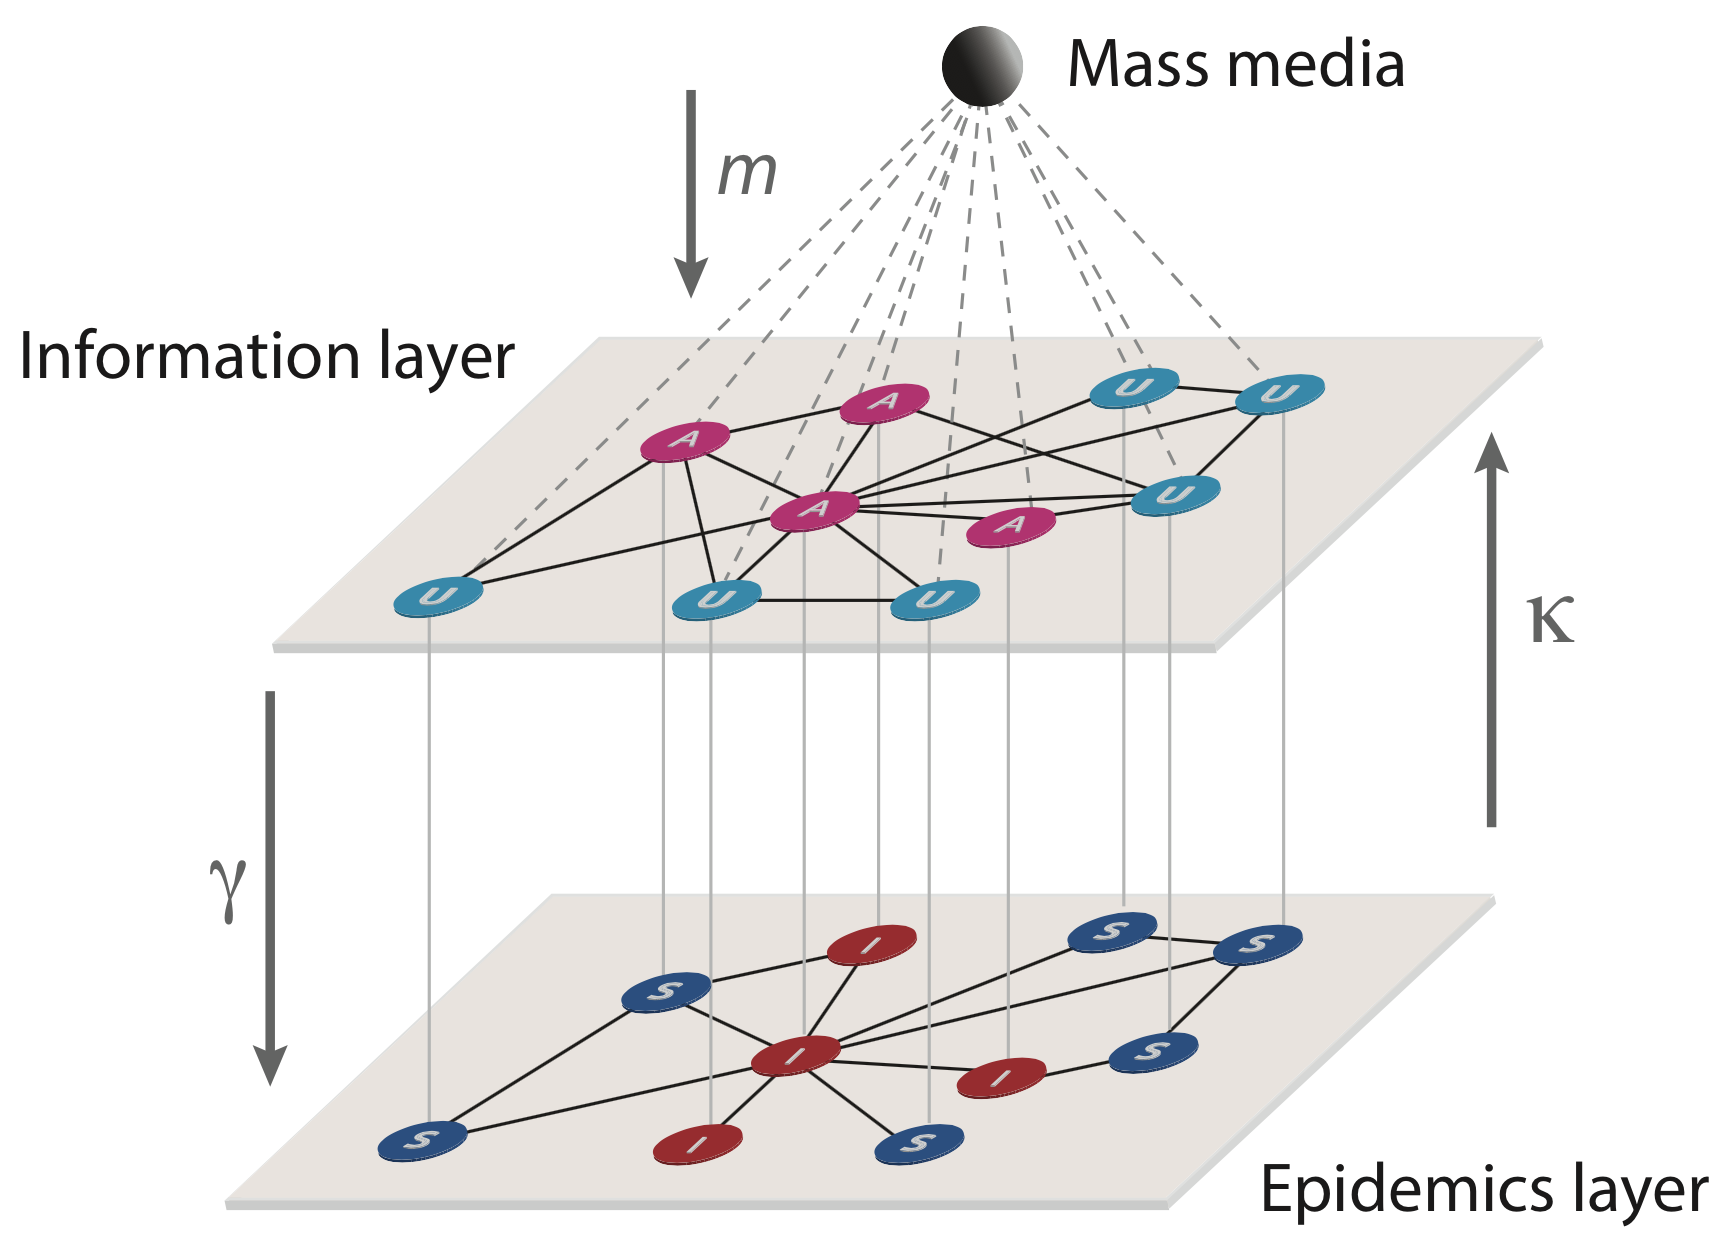
\includegraphics[width=0.7\linewidth]{figs/granell-fig}
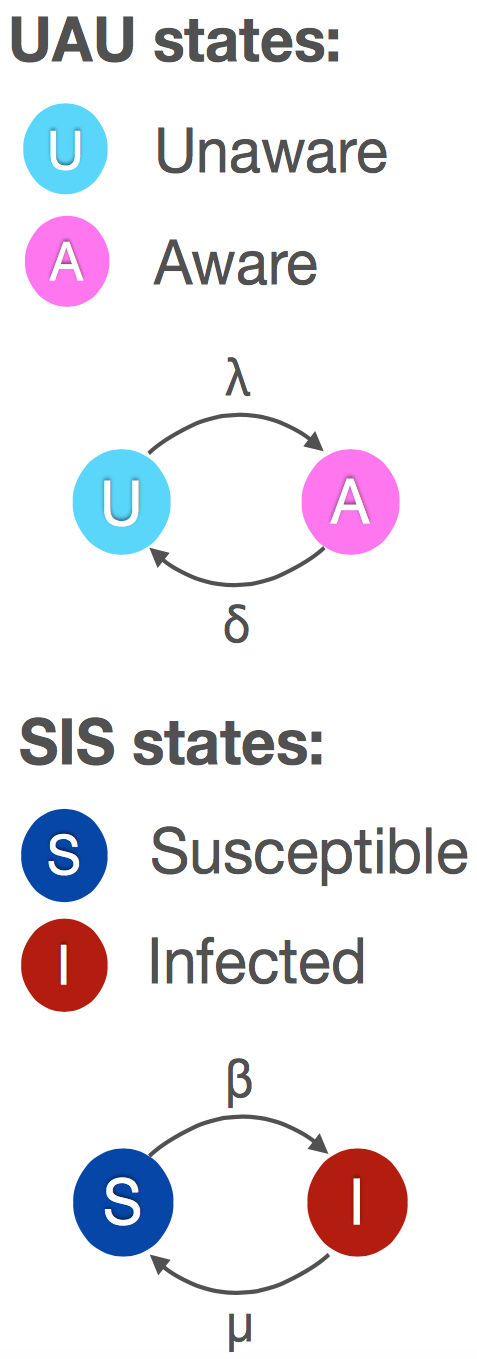
\includegraphics[width=0.18\linewidth]{figs/granell-fig22}
\end{center}
\caption[Awareness-epidemic model in the presence of mass media]{\centering Example application of multiplex networks:\linebreak Awareness-epidemic model in the presence of mass media.}
  \label{figgranell}
\end{figure}

\section{Challenges}\label{secchal}

At the onset of this project, I had no prior knowledge of probabilistic machine learning models or multiplex networks; as such, a major initial challenge involved reading up on large amounts of relevant background material, so I could be properly set to tackle the project. In addition, research in complex networks is a relatively new trend, which meant that there was a lack of textbooks that could be utilised; I had to obtain most of the knowledge in this area by invesetigating relevant academic papers. \\ \\
The main implementation goal of the project has been to adapt known machine learning algorithms and data structures to take advantage of multiplexity; because I wanted to make this as generic as possible and because integrating my project with existing library implementations might be cumbersome and not even work as proposed, I made a decision early on to make the project completely self-contained, implementing all the relevant single-layer machine learning algorithms myself. This resulted in a large codebase, and several subtle bugs and errors had to be taken care of during the implementation stage. Most of them have stemmed from the fact that the implemented algorithms are generally numerical in nature, and a minor error when working with floating-point types can gain much larger significance on the larger scale model's outputs.

\section{Related work}

\subsection{Current research}

Research in multiplex networks is currently highly active, and large quantities of papers are continuously published over the past few years investigating their various features \cite{asllani2014turing, bianconi2013statistical, nicosia2013growing}, applications to modelling real-world systems \cite{estrada2014communicability, granell2014competing, hu2014conditions, zhao2014multiple} or developing novel algorithms on them \cite{azimi2014k, loe2014comparison}.
%A major hub that is responsible for a considerable number of the papers released is the PLEXMATH\footnote{\url{http://www.plexmath.eu}} project; its primary focus is on developing the theory behind multiplex networks, extending known constructs from simpler networks to the multiplex case, and evaluating the approaches using real-world data sets.

\subsection{Multilayer networks library}\label{secnetlib}

This library\footnote{\url{http://www.plexmath.eu/?page_id=327}} builds on the theoretical foundations of multilayer networks outlined in Kivel{\"a} \emph{et al.}\! \cite{kivela2014multilayer}, and implements a basic model of multilayer networks and computing various known metrics on them.\\ \\
As the library is implemented in Python, it is unsuitable for larger data sets, and the algorithms it currently implements are not useful for the kind of problem this project aims to solve. At the time of writing this dissertation, it is, however, the only publicly available generic library implementation of multiplex networks I was able to find.

\subsection{{\tt muxViz}}\label{secmuxviz}

{\tt muxViz}\footnote{\url{http://muxviz.net}} \cite{de2014multilayer} is a software for multiplex network visualisation, utilising R, GNU Octave and OpenGL to produce high-quality 3D representations of the networks.\\ \\
%Some of the additional features of {\tt muxViz} include:
%\begin{itemize}
%	\item Calculations of various metrics (such as \emph{node centrality}, \emph{community detection}, etc.) in order to give a more detailed view of the visualised graph;
%	\item Overlaying the final image, e.g. by a \emph{geographical map} if the nodes contain GPS coordinate information (which is particularly useful for visualising transportation networks);
%	\item \emph{Animating dynamical processes} on the networks, provided the proper temporal data is supplied.
%\end{itemize}
As such visualisations could be very useful for investigating the networks' properties, one of the extensions of the project I have implemented ``dumps'' the generated multiplex network into a format {\tt muxViz} can directly read and analyse.

\chapter{Preparation}

\emph{In this chapter, I will summarise all the preparatory work done before the implementation phase began. To begin, a summary of the initial study phase, in the form of an overview of the theory behind the two prinicipal data structures used in this project (multiplex networks and hidden Markov models), will be presented. The remainder of the chapter will focus on the project planning phases, imperative for successfully executing a project of this magnitude: formally defining the problem to solve, requirements and dependency analysis, choice of tools and software engineering practices.}

\section{Introduction to multiplex networks}\label{secmux}

Within the scope of the project proposal (Appendix \ref{secprop}), I have given a `self-contained' definition of multiplex networks and suggested a possible method of representation for them. In order to be fully precise about this, in this section I will formally define multiplex networks, by first defining their more generalised counterpart, \emph{multilayer networks}, and general constraints that could be imposed on them---once that is done, defining multiplex networks reduces to specifying the required constraints.

\subsection{Multilayer networks}

Before properly defining multilayer networks, it is sensible to start off by revisiting the definition of \textbf{graphs} \cite{bollobas1998modern}, as the main building blocks used to construct them.

\begin{mydef}\label{def:1}
\rm A \emph{graph} (within this context sometimes called a \emph{single-layer} or \emph{monoplex} network) is an ordered pair $G \myeq (V, E)$, where $V$ is a set of \emph{nodes} and $E \subseteq V \times V$ is a set of \emph{edges} that connect pairs of nodes together. 
\end{mydef}

\noindent To extend this notion to multilayer networks, we will retain the concept of a set of nodes $V$ over which the network is built; a \textbf{layer} $G_\alpha \myeq (V_\alpha, E_\alpha)$ of this network can then be defined as a graph over a \emph{subset} of nodes $V_\alpha \subseteq V$; by Definition \ref{def:1} it must hold that $E_\alpha\subseteq V_\alpha \times V_\alpha$. A multilayer network consists of a \textbf{sequence of $L$ layers}, $\mathcal{L} \myeq \left\{G_\alpha\right\}_{\alpha=1}^L$.\\ \\
A node in a multilayer network is uniquely determined by the member of the set $V$ it corresponds to, and the layer it's located in. It is hence reasonable to consider \textbf{node-layer pairs} when defining multilayer networks; the set of all such pairs, $V_M \subseteq V \times \mathcal{L}$ is trivially defined as $V_M \myeq \left\{(x, G_\alpha)\ |\ x \in V_\alpha \right\}$.\\ \\
Lastly, the node-layer pairs may be arbitrarily pairwise connected through {\bf edges}; we define the {\bf set of edges} between node-layer pairs $E_M \subseteq V_M \times V_M$, analogously as before. Using all of the previously defined elements, it is possible to define a multilayer network as follows:

\begin{mydef}\label{def:2}
\rm A \emph{multilayer network} is a 4-tuple $M \myeq (V_M, E_M, V, \mathcal{L})$, where $V$ is a set of nodes contained in the network, $\mathcal{L}$ is the sequence of layers the network consists of, and $V_M$ and $E_M$ are the sets of node-layer pairs and edges between them, respectively.
\end{mydef}

\noindent Essentially, the overall multilayered structure still represents a graph, which can be obtained by extracting the first two elements from the tuple; $G_M \myeq (V_M, E_M)$.\\ \\ %This allows us to easily generalise some of the definitions used for regular graphs for usage within the context of multilayer networks; to name a few examples:
%\begin{itemize}
%	\item A multilayer network $M = (V_M, E_M, V, \mathcal{L})$ is \emph{undirected} if 
%	\[\forall x, y \in V.\ \forall G_\alpha, G_\beta \in \mathcal{L}.\ \left((x, G_\alpha), (y, G_\beta)\right) \in E_M \implies \left((y, G_\beta), (x, G_\alpha)\right) \in E_M\]
%	and \emph{directed} otherwise.
%	\item A \emph{weighted} multilayer network is defined as a 5-tuple $M_w \myeq (V_M, E_M, V, \mathcal{L}, w)$, where the first four elements are defined as for an ordinary multilayer network, and the element $w : E_M \rightarrow \mathbb{R}$ is a \emph{weighting function}, assigning a real-valued \emph{weight} to each edge.
%\end{itemize}
The edges of a multilayer network are usually partitioned into two groups, depending on whether they're contained within a single layer:
\begin{itemize}
	\item The set of \emph{intra-layer} edges, $E_A$, linking together nodes within a single layer;\linebreak $E_A \myeq \left\{((x, G_\alpha), (y, G_\beta)) \in E_M\ |\ \alpha = \beta \right\}$. Note that this set is completely defined by $\mathcal{L}$; that is, $((x, G_\alpha), (y, G_\alpha)) \in E_M \iff (x, y) \in E_\alpha$.
	\item The set of \emph{inter-layer} edges, $E_C$, linking together nodes from different layers;\linebreak $E_C \myeq \left\{((x, G_\alpha), (y, G_\beta)) \in E_M\ |\ \alpha \neq \beta \right\}$.
	\begin{itemize}
		\item It is also helpful to consider a subset of inter-layer edges called the \emph{coupling} edges, $E_{\widetilde{C}} \subseteq E_C$, linking nodes to their own images in different layers;\linebreak $E_{\widetilde{C}} \myeq \left\{((x, G_\alpha), (y, G_\beta)) \in E_C\ |\ x=y \right\}$.
	\end{itemize}
\end{itemize}
An example representation of a multilayer network (as well as its underlying graph, $G_M$) is given in Figure \ref{figmulyr}.\\ \\
After defining all of the previous elements, it is possible to define constraints that may be imposed on a multilayer network's structure.

\begin{figure}[h]
\subfloat[Multilayer network, $M = (V_M, E_M, V, \mathcal{L})$]{%
	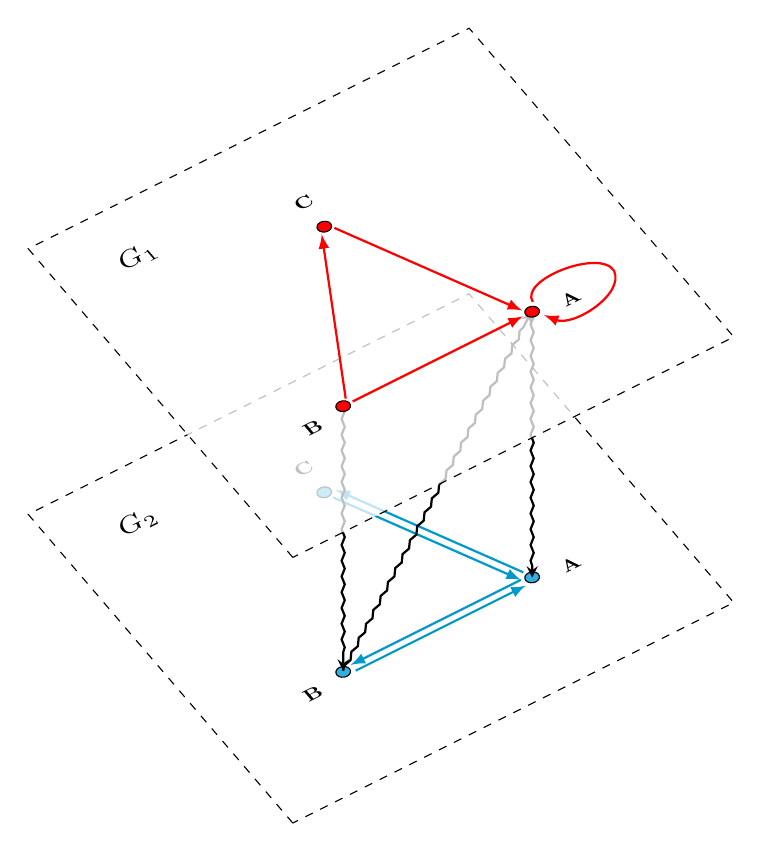
\begin{tikzpicture}[scale=0.8,every node/.style={minimum size=1cm},on grid]
		% Real level
	\begin{scope}[
		yshift=-120,
		every node/.append style={yslant=\yslant,xslant=\xslant},
		yslant=\yslant,xslant=\xslant
	] 
		% The frame:
		\draw[black, dashed, thin] (0,0) rectangle (7,7); 
		% Agents:
		\draw[fill=echoreg]  
			(5,2) node(111){} circle (.1) % Firms
			(2,2) circle (.1) % Households
			(3.5,5) circle (.1); % Banks
		% Flows:
		%\draw[-latex,thin] 
		%	(2,1.8) to[out=-90,in=-90] (5,1.8); % Labour Powers
		%\draw[-latex,thin]
		%	(5,2.2) to[out=90,in=90] (2,2.2); % Wages
		 % Labels:
		 \draw[-latex, thick, color=echodrk]
			(3.55,4.85) to (4.85,2.05);
		 \draw[-latex, thick, color=echodrk]
			(4.95,2.15) to (3.65,4.95);
		\draw[-latex, thick, color=echodrk]
			(2.15,1.92) to (4.85,1.92); % Consumption
		\draw[-latex, thick, color=echodrk]
			(4.85,2.05) to (2.15,2.05); % Consumption
		\fill[black]
			(0.5,6) node[right, scale=1] {$G_2$}	
			(5.1,1.9) node[right,scale=.7]{\bf A}
			(1.9,1.9) node[left,scale=.7]{\bf B}
			(3.5,5.1) node[above,scale=.7]{\bf C};	
	\end{scope}
	
	% 2 vertical lines for linking agents on the 2 levels
	\draw[thick, -stealth, decoration={snake, segment length=2mm, amplitude=0.2mm, post length=1.5mm}, decorate] (3.8, 3.9) to (3.8, -0.32);
	\draw[thick, -stealth, decoration={snake, segment length=2mm, amplitude=0.2mm, post length=1.5mm}, decorate] (.8,2.4) to (.8,-1.8);
	\draw[thick, -stealth, decoration={snake, segment length=2mm, amplitude=0.2mm, post length=1.5mm}, decorate] (.8, -1.8) to (3.79, 3.9);
	
	% Monetary level
	\begin{scope}[
		yshift=0,
		every node/.append style={yslant=\yslant,xslant=\xslant},
		yslant=\yslant,xslant=\xslant
	]
		% The frame:
		\fill[white,fill opacity=.75] (0,0) rectangle (7,7); % Opacity
		\draw[black, dashed, thin] (0,0) rectangle (7,7); 
		 % Agents:
		\draw [fill=red]
			(5,2) node(111){} circle (.1) % Firms
			(2,2) circle (.1) % Households
			(3.5,5) circle (.1); % Banks
		 % Monetary Flows:
		\draw[-latex, thick, color=red]
			(3.6,4.9) to (4.9,2.1);
		\draw[-latex, thick, color=red]
			(2.15,2) to (4.85,2); % Consumption
		\draw[-latex, thick, color=red]
			(2.1,2.1) to (3.4,4.9) ; % Repayments
		\draw[-latex, thick, color=red]
			(5.1,2.15) to[bend left=90] (6.3, 2) to[bend left=70] (5.1, 1.85) ; % Repayments
		 % Labels:
		\fill[black]
			(0.5,6) node[right, scale=1] {$G_1$}
			(5.1,1.9) node[right,scale=.7]{\bf A}
			(1.9,1.9) node[left,scale=.7]{\bf B}
			(3.5,5.1) node[above,scale=.7]{\bf C}; 
	\end{scope} 
	\end{tikzpicture}
}
\quad
\subfloat[Underlying graph, $G_M = (V_M, E_M)$]{
	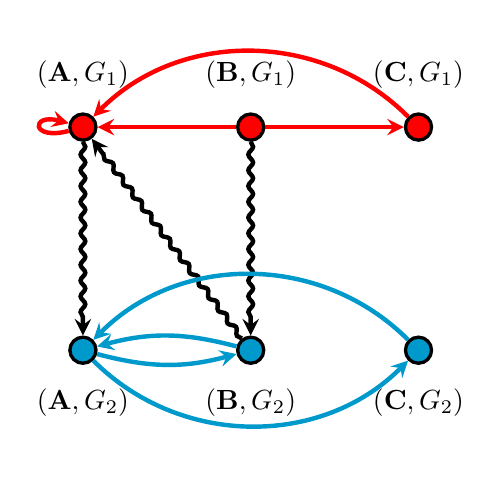
\begin{tikzpicture}
		\node[circle, draw, very thick, fill=echodrk] (11) {};
		\node[below = 0.5em of 11] (11c) {$({\bf A}, G_2)$};
		\node[circle, draw, very thick, fill=echodrk, right=5em of 11] (22) {};
		\node[below =0.5em of 22] (22c) {$({\bf B}, G_2)$};
		\node[circle, draw, very thick, fill=echodrk, right=5em of 22] (33) {};
		\node[below =0.5em of 33] (33c) {$({\bf C}, G_2)$};
		\node[circle, draw, very thick, fill=red, above = 7em of 11] (1) {};
		\node[above = 0.5em of 1] (1c) {$({\bf A}, G_1)$};
		\node[circle, draw, very thick, fill=red, right=5em of 1] (2) {};
		\node[above =0.5em of 2] (2c) {$({\bf B}, G_1)$};
		\node[circle, draw, very thick, fill=red, right=5em of 2] (3) {};
		\node[above =0.5em of 3] (3c) {$({\bf C}, G_1)$};
		
		\draw[ultra thick, -stealth, decoration={snake, segment length=2mm, amplitude=0.3mm, post length=1.5mm}, decorate] (1) to (11);
		\draw[ultra thick, -stealth, decoration={snake, segment length=2mm, amplitude=0.3mm, post length=1.5mm}, decorate] (2) to (22);
		\draw[ultra thick, -stealth, decoration={snake, segment length=2mm, amplitude=0.3mm, post length=1.5mm}, decorate] (22) to (1);
		
		\draw[-stealth, ultra thick, bend right=15, color=echodrk] (11) to (22); % Consumption
		\draw[-stealth, ultra thick, bend right=15, color=echodrk] (22) to (11); % Consumption
		\draw[-stealth, ultra thick, bend right=45, color=echodrk] (11) to (33); % Consumption
		\draw[-stealth, ultra thick, bend right=45, color=echodrk] (33) to (11); % Consumption
		
		\draw[-stealth, ultra thick, color=red] (2) to (1); % Consumption
		\draw[-stealth, ultra thick, color=red] (2) to (3); % Consumption
		\draw[-stealth, ultra thick, bend right=45, color=red] (3) to (1); % Consumption
		
		\draw[-stealth, ultra thick, loop left, color=red] (1) to (1);
	\end{tikzpicture}}
	\caption[Example of a multilayer network and its underlying graph]{\centering
	Example of a multilayer network (a) and its underlying graph (b).}
	\label{figmulyr}
\end{figure}

\subsection{Constraints}

Some of the constraints that may be imposed on a multilayer network are as follows \cite{kivela2014multilayer}:
\begin{itemize}
	\item A multilayer network is \emph{node-aligned} if every layer contains all the nodes; \linebreak i.e. $\forall G_\alpha = (V_\alpha, E_\alpha) \in \mathcal{L}.\ V_\alpha = V$. The network given in Figure \ref{figmulyr} is node-aligned; both layers ($G_1$ and $G_2$) contain all three nodes ($\left\{{\bf A}, {\bf B}, {\bf C}\right\}$).
%	\item A multilayer network is \emph{layer-disjoint} if each node appears in at most one layer; \linebreak i.e. $\forall x \in V.\ \forall G_\alpha, G_\beta \in \mathcal{L}.\  (x, G_\alpha) \in V_M \wedge (x, G_\beta) \in V_M \implies \alpha = \beta$. The network given in Figure \ref{figmulyr} is not layer-disjoint, because e.g.\! node ${\bf A}$ appears in both $G_1$ and $G_2$.
	\item A multilayer network is \emph{diagonally coupled} if all inter-layer edges are coupling, \linebreak i.e. $E_C = E_{\widetilde{C}}$. The network given in Figure \ref{figmulyr} is not diagonally coupled, because the edge $\left(\left({\bf B}, G_2\right), \left({\bf A}, G_1\right)\right)$ is not coupling.
%	\item A weighted diagonally coupled multilayer network is \emph{layer-coupled} if the weights of the coupling edges are independent of the nodes; \linebreak i.e. $\forall x, y \in V.\ \forall G_\alpha, G_\beta \in \mathcal{L}.\  w((x, G_\alpha), (x, G_\beta)) = w((y, G_\alpha), (y, G_\beta))$.
	\item A diagonally coupled multilayer network is \emph{categorically coupled} if each node is connected to \emph{all} of its images in the other layers; i.e. $\forall x \in V.\ \forall G_\alpha, G_\beta \in \mathcal{L}.\linebreak  (x, G_\alpha) \in V_M \wedge (x, G_\beta) \in V_M \wedge \alpha \neq \beta \implies ((x, G_\alpha), (x, G_\beta)) \in E_M$.
\end{itemize}

\subsection{Multiplex networks}\label{secmuxnet}

With the previously defined framework, it is simple to formally define a multiplex network, which also concludes this section.
\begin{mydef}\label{def:mux}
\rm A \emph{multiplex network} is a node-aligned, diagonally coupled multilayer network.
\end{mydef}

\noindent From Definition \ref{def:mux} it follows that, to define an instance of a multiplex network, it is sufficient to specify $V$, $\mathcal{L}$ and $E_{\widetilde{C}}$. Furthermore, if the coupling is of a special type, $E_{\widetilde{C}}$ is no longer needed (this is the case for e.g. the previously mentioned \emph{categorical} coupling). Figure \ref{figmultiplex} represents an example categorical multiplex network.

\begin{figure}[h]
\subfloat[Categorical multiplex network, $M = (V, \mathcal{L})$]{%
	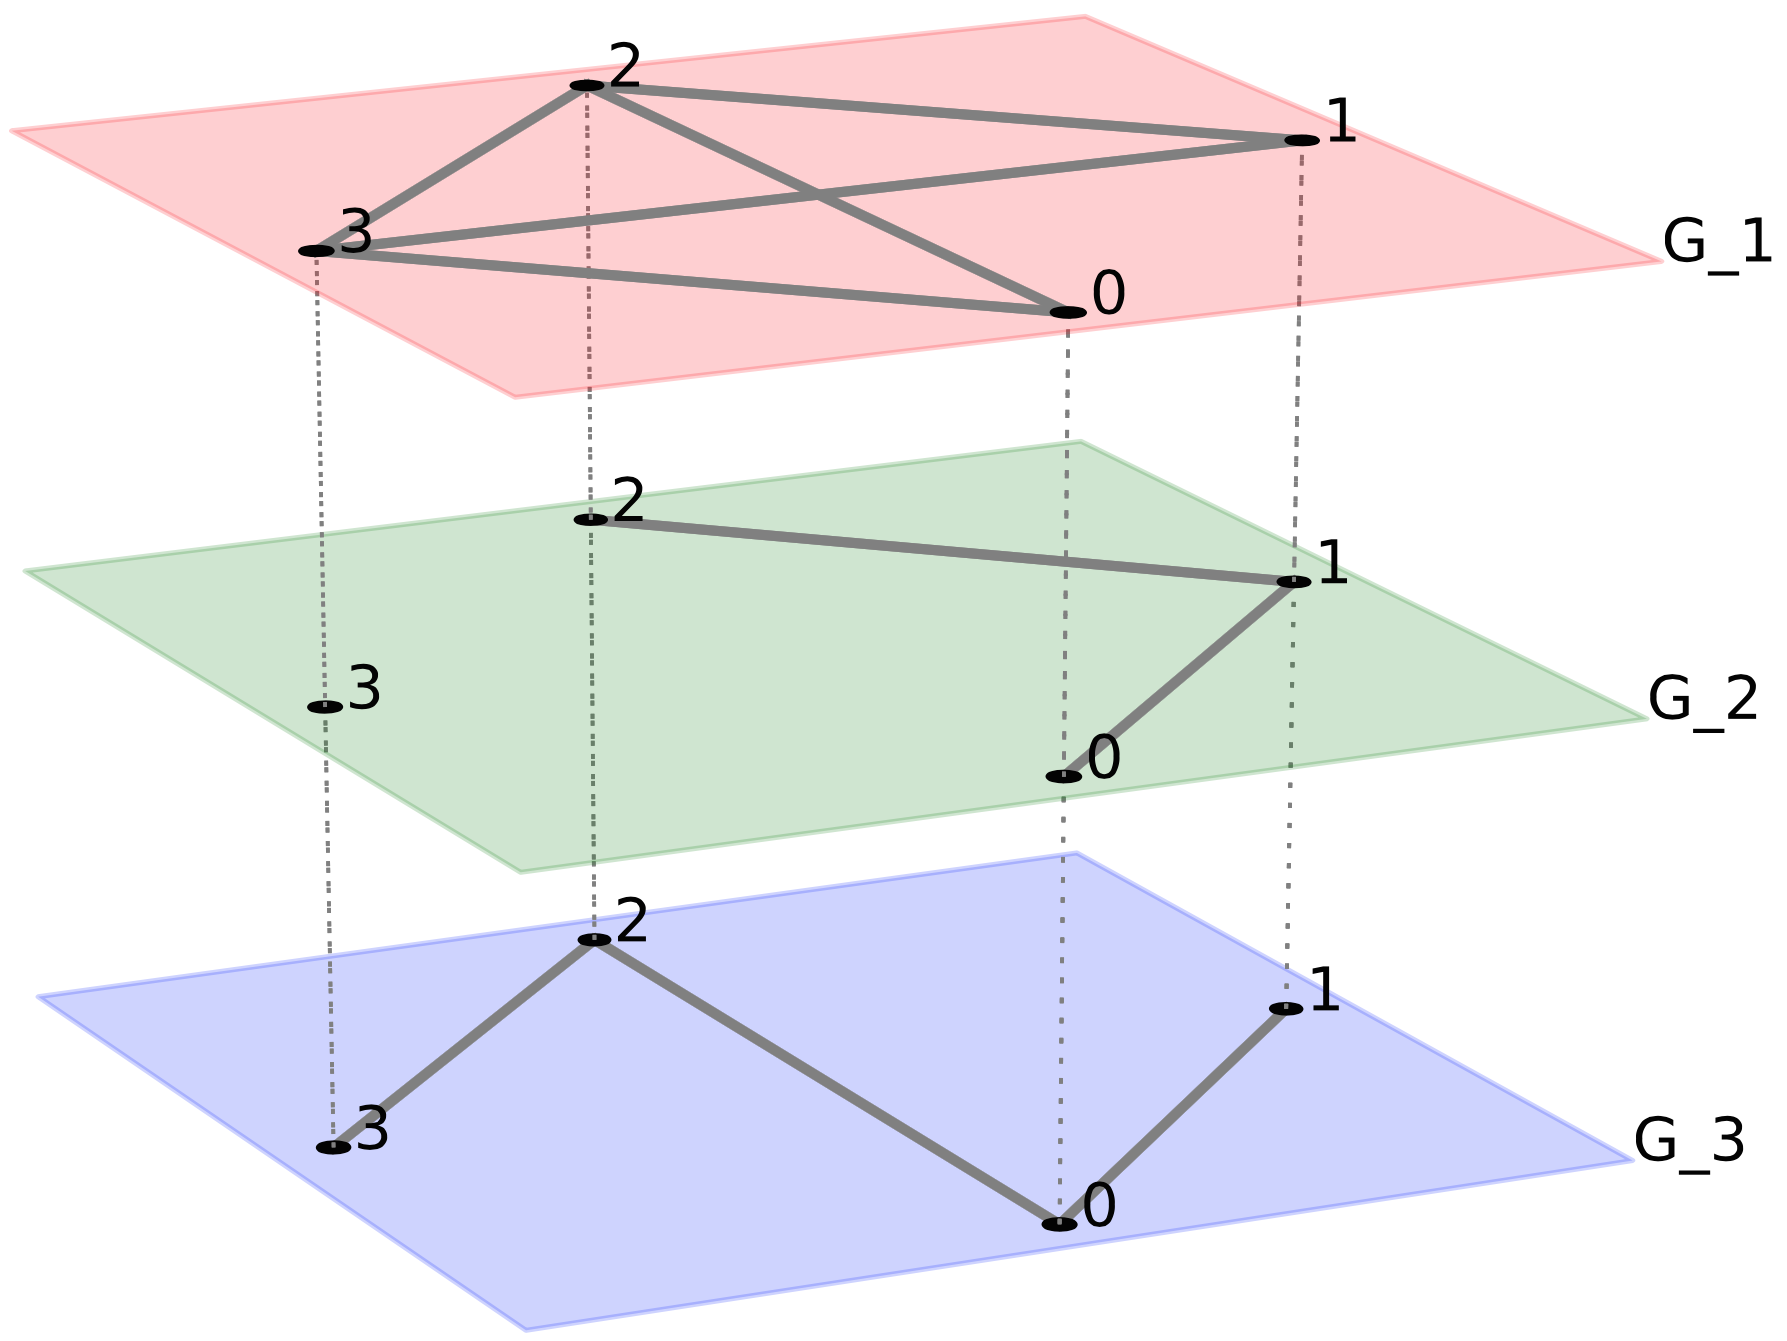
\includegraphics[width=0.5\linewidth]{figs/mux-genfig}
}
\quad
\subfloat[Underlying graph, $G_M = (V_M, E_M)$]{
	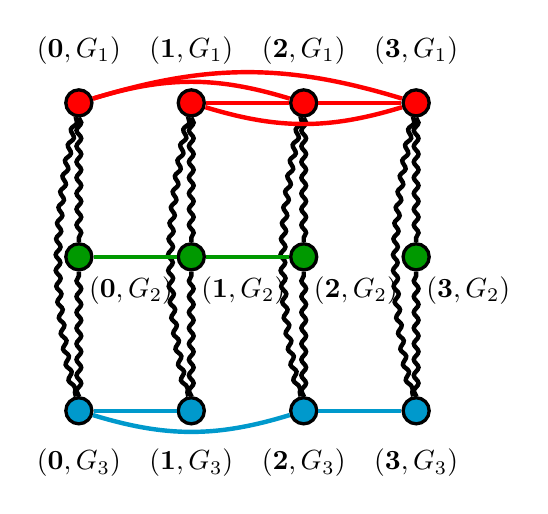
\begin{tikzpicture}
		\node[circle, draw, very thick, fill=echodrk] (11) {};
		\node[below = 0.5em of 11] (11c) {$({\bf 0}, G_3)$};
		\node[circle, draw, very thick, fill=echodrk, right=3em of 11] (22) {};
		\node[below =0.5em of 22] (22c) {$({\bf 1}, G_3)$};
		\node[circle, draw, very thick, fill=echodrk, right=3em of 22] (33) {};
		\node[below =0.5em of 33] (33c) {$({\bf 2}, G_3)$};
		\node[circle, draw, very thick, fill=echodrk, right=3em of 33] (44) {};
		\node[below =0.5em of 44] (44c) {$({\bf 3}, G_3)$};
		
		\node[circle, draw, very thick, fill=mygreen, above = 4.5em of 11] (111) {};
     	\node at ([shift={(0.53,-0.3)}]111.-45) {$({\bf 0}, G_2)$};
		\node[circle, draw, very thick, fill=mygreen, right=3em of 111] (222) {};
     	\node at ([shift={(0.53,-0.3)}]222.-45) {$({\bf 1}, G_2)$};
		\node[circle, draw, very thick, fill=mygreen, right=3em of 222] (333) {};
     	\node at ([shift={(0.53,-0.3)}]333.-45) {$({\bf 2}, G_2)$};
		\node[circle, draw, very thick, fill=mygreen, right=3em of 333] (444) {};
     	\node at ([shift={(0.53,-0.3)}]444.-45) {$({\bf 3}, G_2)$};
		
		\node[circle, draw, very thick, fill=red, above = 4.5em of 111] (1) {};
		\node[above = 0.5em of 1] (1c) {$({\bf 0}, G_1)$};
		\node[circle, draw, very thick, fill=red, right=3em of 1] (2) {};
		\node[above =0.5em of 2] (2c) {$({\bf 1}, G_1)$};
		\node[circle, draw, very thick, fill=red, right=3em of 2] (3) {};
		\node[above =0.5em of 3] (3c) {$({\bf 2}, G_1)$};
		\node[circle, draw, very thick, fill=red, right=3em of 3] (4) {};
		\node[above =0.5em of 4] (3c) {$({\bf 3}, G_1)$};
		
		
		\draw[ultra thick, -, decoration={snake, pre length=0.01mm, segment length=2mm, amplitude=0.3mm, post length=0.2mm}, decorate] (11) to (111);
		\draw[ultra thick, -, decoration={snake, pre length=0.01mm, segment length=2mm, amplitude=0.3mm, post length=0.2mm}, decorate] (22) to (222);
		\draw[ultra thick, -, decoration={snake, pre length=0.01mm, segment length=2mm, amplitude=0.3mm, post length=0.2mm}, decorate] (33) to (333);
		\draw[ultra thick, -, decoration={snake, pre length=0.01mm, segment length=2mm, amplitude=0.3mm, post length=0.2mm}, decorate] (44) to (444);
		
		\draw[ultra thick, -, decoration={snake, pre length=0.01mm, segment length=2mm, amplitude=0.3mm, post length=0.2mm}, decorate] (1) to (111);
		\draw[ultra thick, -, decoration={snake, pre length=0.01mm, segment length=2mm, amplitude=0.3mm, post length=0.2mm}, decorate] (2) to (222);
		\draw[ultra thick, -, decoration={snake, pre length=0.01mm, segment length=2mm, amplitude=0.3mm, post length=0.2mm}, decorate] (3) to (333);
		\draw[ultra thick, -, decoration={snake, pre length=0.01mm, segment length=2mm, amplitude=0.3mm, post length=0.2mm}, decorate] (4) to (444);
		
		
		
		\draw[ultra thick, -, bend right=12, decoration={snake, pre length=0.01mm, segment length=2mm, amplitude=0.3mm, post length=0.2mm}, decorate] (1) to (11);
		\draw[ultra thick, -, bend right=12, decoration={snake, pre length=0.01mm, segment length=2mm, amplitude=0.3mm, post length=0.2mm}, decorate] (2) to (22);
		\draw[ultra thick, -, bend right=12, decoration={snake, pre length=0.01mm, segment length=2mm, amplitude=0.3mm, post length=0.2mm}, decorate] (3) to (33);
		\draw[ultra thick, -, bend right=12, decoration={snake, pre length=0.01mm, segment length=2mm, amplitude=0.3mm, post length=0.2mm}, decorate] (4) to (44);
		
		\draw[-, ultra thick, color=echodrk] (11) to (22); % Consumption
		\draw[-, ultra thick, bend right=17, color=echodrk] (11) to (33); % Consumption
		\draw[-, ultra thick, color=echodrk] (33) to (44); % Consumption
		
		\draw[-, ultra thick, color=mygreen] (111) to (222); % Consumption
		\draw[-, ultra thick, color=mygreen] (222) to (333); % Consumption
		
		\draw[-, ultra thick, bend left=17, color=red] (1) to (3); % Consumption
		\draw[-, ultra thick, bend left=17, color=red] (1) to (4); % Consumption
		\draw[-, ultra thick, bend right=17, color=red] (2) to (4); % Consumption
		\draw[-, ultra thick, color=red] (2) to (3); % Consumption
		\draw[-, ultra thick, color=red] (3) to (4); % Consumption
		
	\end{tikzpicture}}
	\caption[Example of a categorical multiplex network and its underlying graph]{\centering
	Example of a categorical undirected multiplex network\footnotemark[2] (a) and its underlying graph (b).}
	\label{figmultiplex}
\end{figure}

\section{Gaussian mixture hidden Markov models}

Having assimilated the material on the various kinds of multilayer networks, I was prepared to attempt to apply the multiplexity phenomenon to a machine learning model. After researching several alternatives, I opted for {\bf hidden Markov models} (\emph{HMM}s) \cite{baum1966statistical, baum1970maximization}, for two primary reasons:
\begin{itemize} 
	\item They are a fairly simple model to comprehend and implement, but have been proven to be powerful for many pattern-recognition tasks \cite{pardo2005modeling, satish1993use, starner1995real};
	\item Combining multiple HMMs with the use of a multiplex network lends itself to a relatively simple implementation and a straightforward justification (as will be described in \cref{secmuxchaiin}).
\end{itemize}
\footnotetext[2]{The multiplex network has been generated and drawn using the \emph{multilayer networks library} (\cref{secnetlib}).}\stepcounter{footnote}\stepcounter{footnote}
Hidden Markov models are a principal component of several CST Part II courses' syllabi (\emph{Artificial Intelligence II}, \emph{Bioinformatics}, \emph{Natural Language Processing}\dots), and as such their formal definition details are omitted from the main dissertation body; a thorough discussion is given in Appendix \ref{secintrohmm}.\\ \\
This project utilises an extension to HMMs---namely, the \emph{Gaussian mixture} HMM (\emph{GMHMM}). The need for such a model has arisen primarily from my intent to handle \emph{continuous outputs}; I opted for this approach because most of the experimentally observable data (including the biomolecular data designated for evaluation) is continuous---an implementation like this could prove to be more easily \emph{reusable} (without having to modify much, if any, code) for scientists in a variety of different fields.\\ \\
A GMHMM consists of a set of states, $S$, a set of ``sub-outputs'', $O'$. The system follows a particular sequence of states (with a \emph{transition probability matrix}, $\bf T$, specifying the probabilities of transitioning between each pair of states), with each state emitting a sub-output, which in turn emits an output value that may be observed. Therefore, each state has associated with it the probabilities of emitting each sub-output (defined by an \emph{emission probability matrix}, $\bf O'$), and each sub-output $y'$ has its own parameters for a Gaussian distribution (mean $\mu_{y'}$ and standard deviation $\sigma_{y'}$) used to produce its corresponding outputs. Figure \ref{figgmhmm} depicts an example of a GMHMM.
\begin{figure}[H]
\centering 	
%TC:ignore
\begin{tikzpicture}[-stealth,very thick,node distance = 4cm,auto]

    \node[state] (x) {$x$};
    \node[state] (y) [above right of=x] {$y$};
    \node[state] (z) [below right of=y] {$z$};
    
    \node[rectangle, minimum size=2em,draw] (a) [above left =of y] {$a$};
    \node[rectangle,minimum size=2em, draw] (b) [above = of y] {$b$};
    \node[rectangle, minimum size=2em,draw] (c) [above right =of y] {$c$};

	\draw[] (x) to node[above left] {$1$} (y);
	\draw[loop above] (y) to node {$0.5$} (y);
	\draw[bend left=20] (y) to node {$0.5$} (z);
	\draw[bend left=20] (z) to node[below left] {$0.7$} (y);
	\draw[] (z) to node {$0.3$} (x);
	
	\draw[dashed] (x) to node[left] {$0.9$} (a);
	\draw[dashed] (x) to node[left] {$0.1$} (b);
	\draw[bend right=30, dashed] (y) to node[right] {$0.6$} (b);
	\draw[dashed] (y) to node[below right] {$0.4$} (c);
	\draw[dashed] (z) to node[right] {$1$} (c);
\node[rectangle, draw, scale=0.2, minimum size=20em,above = 2cm of a] (ga){\begin{tikzpicture}
\begin{axis}[axis lines=none, ticks=none,xmax=3, xmin=-3,ymax=1.1]
\addplot[ultra thick,black, no markers,samples=200] {exp(-x^2)};
\end{axis}\end{tikzpicture}};
\node[rectangle, draw, scale=0.2, minimum size=20em,above = 2cm of b] (gb){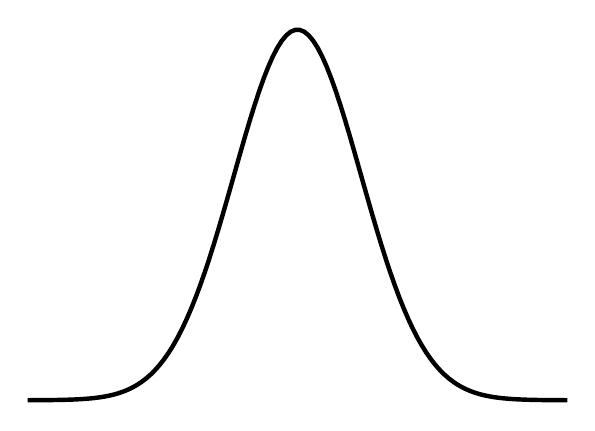
\begin{tikzpicture}
\begin{axis}[axis lines=none, ticks=none,xmax=3, xmin=-3,ymax=1.1]
\addplot[ultra thick,black, no markers,samples=200] {exp(-x^2)};
\end{axis}\end{tikzpicture}};
\node[rectangle, draw, scale=0.2, minimum size=20em,above = 2cm of c] (gc){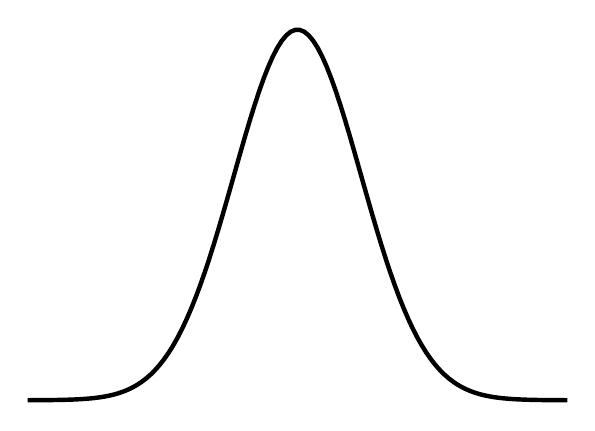
\begin{tikzpicture}
\begin{axis}[axis lines=none, ticks=none,xmax=3, xmin=-3,ymax=1.1]
\addplot[ultra thick,black, no markers,samples=200] {exp(-x^2)};
\end{axis}\end{tikzpicture}};

\draw[dotted, bend left] (a) to node[left] {$\mu_a$} (ga);
\draw[dotted, bend right] (a) to node[right] {$\sigma_a$} (ga);
\draw[dotted, bend left] (b) to node[left] {$\mu_b$} (gb);
\draw[dotted, bend right] (b) to node[right] {$\sigma_b$} (gb);
\draw[dotted, bend left] (c) to node[left] {$\mu_c$} (gc);
\draw[dotted, bend right] (c) to node[right] {$\sigma_c$} (gc);

\end{tikzpicture}
%TC:endignore
\caption[Example of a Gaussian mixture hidden Markov model]{\centering Example of a Gaussian mixture hidden Markov model, with the state set $S=\{x, y, z\}$, and sub-output set $O'=\{a, b, c\}$.}\label{figgmhmm}
\end{figure}

%\noindent The primary reason for deciding to implement this extension in my project is twofold:
%\begin{itemize} 
%	\item The way the proposed evaluation data set is organised assumes that the observed output is dependent on an underlying layer of (invisible) sub-output;
%	\item The model provides more \emph{flexibility} compared to the simple Gaussian HMM, so it is more likely to be useful to others.
%\end{itemize}

\section{Requirements analysis}\label{secreq}

Upon successful comprehension of the background material, I refined the {\bf success criteria} originally given in the project proposal (Appendix \ref{secprop}) into a {\bf statement of the primary problem} that the project intends to solve, along with a set of {\bf deliverables} that should be produced to that end, with their respective {\bf priorities} and mutual {\bf dependencies}.\\ \\
The statement of the primary problem is as follows:
\begin{framed}
	\noindent \textbf{Given two classes, $C_1$ and $C_2$, and two paired vectors of real-valued observations, $\vec{x}$ and $\vec{y}$ (such that $x_i$ and $y_i$ represent different measurements ($\sim$ \emph{data types}) on the same entity, or on the same point in time), determine whether the pair $(\vec{x}, \vec{y})$ is a member of $C_1$ or $C_2$}.
\end{framed}
\noindent This represents a \emph{binary classification} problem, where the input to be classified consists of two types of data. For example, in the context of diagnostics, $C_1$ could refer to `patient' and $C_2$ to `normal', and $\vec{x}$ and $\vec{y}$ could refer to two types of measurements obtained from a particular subject, such that $x_i$ and $y_i$ were measured at the same time (e.g. from the same blood draw). This formulation has been chosen primarily with evaluation in mind, as there exists a wide variety of established metrics for evaluating binary classifiers \cite{powers2011evaluation}.\\ \\
The list of deliverables for the project is outlined in Table \ref{tbldeliv}. Most of them are explicitly mentioned in the project proposal, with a few additions and removals.
\begin{table}[H]\centering
\begin{tabular}{ l  c  c } \toprule
{\bf Deliverable} & {\bf Priority} & {\bf Difficulty}\\ \midrule
Basic chain (GM)HMM implementation & \textcolor{red}{\bf P0} & \textcolor{orange}{\bf Medium}\\
Multiplex network implementation & \textcolor{red}{\bf P0} & \textcolor{orange}{\bf Medium}\\
Multiobjective optimisation algorithm & \textcolor{red}{\bf P0} & \textcolor{red}{\bf High}\\
Multiplex chain GMHMM (integrating all of the above) & \textcolor{red}{\bf P0} & \textcolor{orange}{\bf Medium}\\
Evaluation suite & \textcolor{red}{\bf P0} & \textcolor{red}{\bf High}\\
Full multiplex GMHMM implementation & \textcolor{orange}{\bf P1} & \textcolor{red}{\bf High}\\
%Aggregate multiplex network model & \textcolor{orange}{\bf P1} & \textcolor{red}{\bf High}\\
Noise testing suite & \textcolor{orange}{\bf P1} & \textcolor{orange}{\bf Medium}\\
Multiplex network visualisation (via \texttt{muxViz} (\cref{secmuxviz})) & \textcolor{mygreen}{\bf P2} & \textcolor{mygreen}{\bf Low}\\
Synthetic data generator (for evaluation) & \textcolor{mygreen}{\bf P2} & \textcolor{mygreen}{\bf Low}\\
\bottomrule
\end{tabular}
\caption{A summary of the deliverables within this project.}\label{tbldeliv}
\end{table}
\noindent Deliverables with priority \textcolor{red}{\bf P0} are needed for the {\bf core project}---construction of a basic classifier model and evaluating its performance with the addition of multiplexity---and their proper execution represents the primary success criterion; priorities \textcolor{orange}{\bf P1} and \textcolor{mygreen}{\bf P2} represent the strongly desirable and desirable {\bf extensions}, respectively.\\ \\
Dependency analysis (the results of which are outlined in Figure \ref{figdep}) revealed that the three main building blocks of the project are \emph{independent} (allowing for an inherently {\bf modular} design); integrating them into a single model requires an interface to all three, and the evaluation suite requires an interface to the integrated structure. There were no interdependencies discovered between the deliverables with priorities \textcolor{orange}{\bf P1} and \textcolor{mygreen}{\bf P2}, which meant that the extensions could be implemented in any order after the core elements were in place.
\begin{figure}[h]
\centering
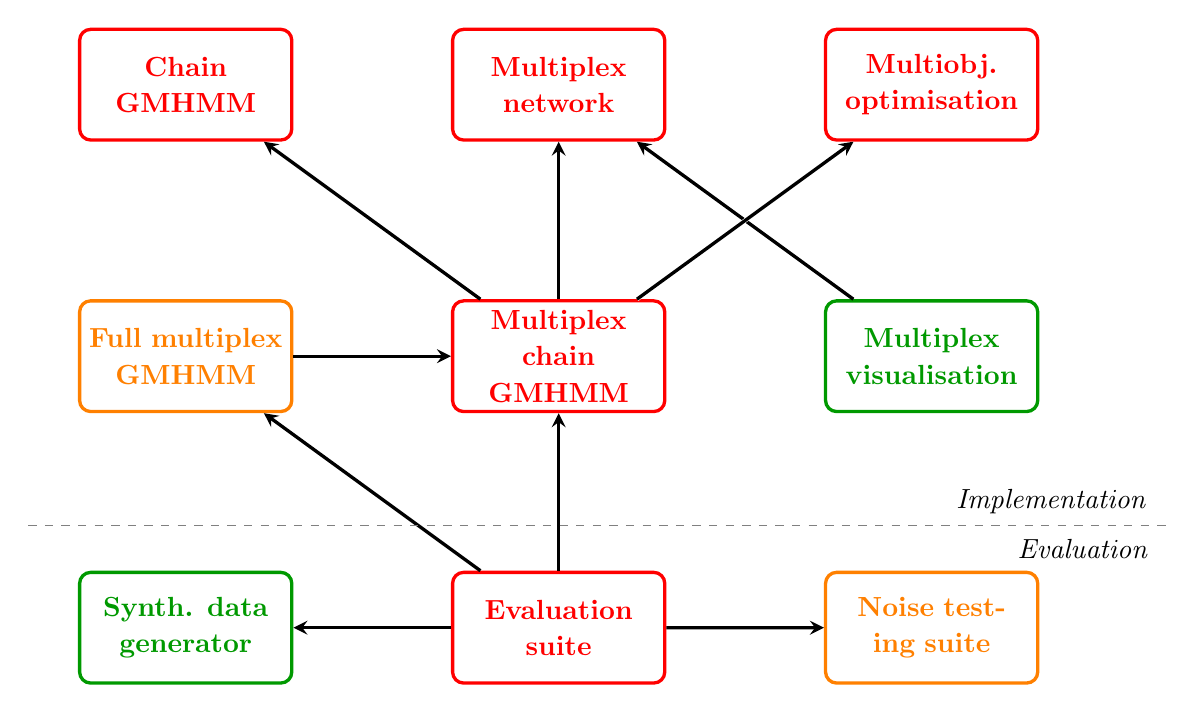
\begin{tikzpicture}[node distance=2cm, auto]
    % Place nodes

    \node [block, very thick, color=red, fill=white] (chn) {\bf Chain GMHMM};
    \node [block, very thick, color=red, fill=white, right = of chn] (mux) {\bf Multiplex network};
    \node [block, very thick, color=red, fill=white, right = of mux] (opt) {\bf Multiobj. optimisation};    
    \node [block, very thick, color=red, fill=white, below = of mux] (mcg) {\bf Multiplex chain GMHMM};       
    \node [block, very thick, color=red, fill=white, below = of mcg] (evl) {\bf Evaluation suite};       
    \node [block, very thick, color=orange, fill=white, left = of mcg] (hmm) {\bf Full multiplex GMHMM};  
    %\node [block, very thick, color=orange, fill=white, right = of mcg] (agg) {\bf Aggregate multiplex model}; 
    \node [block, very thick, color=mygreen, fill=white, right = of mcg] (viz) {\bf Multiplex visualisation}; 
    \node [block, very thick, color=orange, fill=white, below = of viz] (noi) {\bf Noise testing suite}; 
    \node [block, very thick, color=mygreen, fill=white, left = of evl] (alt) {\bf Synth. data generator}; 
    \draw [line] (mcg) -- (chn);
    \draw [line] (mcg) -- (mux);
    \draw [line] (evl) -- (mcg);
    \draw [line] (hmm) -- (mcg);
    \draw [line] (evl) -- (hmm);
    %\draw [line] (agg) -- (mux);
    \draw [line] (viz) -- (mux);
    \draw [-stealth, ultra thick, white] (mcg) -- (opt);
    \draw [line] (mcg) -- (opt);
    %\draw [line] (agg) -- (opt);
    %\draw [line] (evl) -- (agg);
    \draw [line] (evl) -- (noi);
    \draw [line] (evl) -- (alt);
    
    %\draw[step=1.0,black,thin] (-2,-6) grid (12.5,0);
    \draw[dashed, gray] (-2, -5.6) -- (12.5, -5.6);
    \node[align=right] at (11, -5.3) {\emph{Implementation}};
    \node[align=right] at (11.4, -5.9) {\emph{Evaluation}};
\end{tikzpicture}
	\caption[Results of the dependency analysis]{\centering The dependencies found between the components of the project.\linebreak The colour of a component represents its priority level (\textcolor{red}{\bf High} to \textcolor{mygreen}{\bf Low}). \linebreak A directed edge $x \longrightarrow y$ means $x$ is dependent on $y$.}\label{figdep}
\end{figure}

\section{Choice of tools}

\subsection{Programming languages and libraries}

There was a wide variety of programming languages I could have used for accomplishing the tasks outlined above; however, to me it was clear from the onset that the language to be used should be \textbf{\CC}\ \cite{Stroustrup:2000:CPL:518791}, mainly for the reasons of:
\begin{itemize}
	\item \emph{Efficiency}; I wanted to make the final product capable of efficiently handling large data sets---and the C/\CC\ languages were designed with performance and efficiency as their primary goals;
	\item \emph{Proficiency}; At the time of proposing the project, I was already highly familiar with \CC, using it mostly for the purpose of algorithmic programming competitions as well as implementing a variety of data structures and algorithms\footnote{\url{https://github.com/PetarV-/Algorithms}}. 
	\item \emph{Standard Template Library}; \CC\ offers a selection of higher-level constructs and implemented data structures and algorithms, as part of the STL.
\end{itemize}
As mentioned in \cref{secchal}, the project was not expected to rely on any external libraries for the core implementation; as such, I only used the constructs available within the \CC11 STL for the project implementation. For the purpose of executing the test harnesses on the components of the model, several {\bf shell scripts} were written.

\subsection{Development environment}
The entirety of the implementation, evaluation and dissertation writeup work has been carried out on my own machine (2.6 GHz Intel Core i7 with 8 GB RAM, running Mac OS X 10.10 \emph{Yosemite}). The full list of tools utilised for developing the project and writing up the dissertation is given in Table \ref{tbldevtools}. 
\begin{table}[H]\centering
\begin{tabular}{ l  l } \toprule
{\bf Tool} & {\bf Purpose}\\ \midrule
{\tt vim 7.3} & Text editor\\
{\tt Xcode 6.1} & IDE\\
{\tt clang 3.6} & Compiler\\
{\tt GNU Make 3.81} & Build automation\\
{\tt git 2.3.2} & Revision control\\
{\tt rsync 2.6.9} & File transfer\\
{\tt cron} & Job scheduling\\
\TeX pad 1.7.9 & \LaTeX\ editor\\
PGF/Ti{\it k}Z 3.0 & Graphics package\\
{\tt gnuplot 5.0} & Graphing utility\\
\bottomrule
\end{tabular}
\caption{Tools used for the development of the project.}\label{tbldevtools}
\end{table}

\subsection{Backup strategy}

Special attention has been given to devising a resilient backup strategy for this project's codebase and dissertation sources. Using the \texttt{git} revision control system allowed me to store a backup of my repository on the hosting service \emph{GitHub}. For redundancy, I also setup an automatic synchronisation of the project onto my personal file spaces on \emph{Dropbox} and \emph{Google Drive}, utilising \texttt{rsync} and \texttt{cron}. Lastly, I also made regular manual backups of my machine's entire filesystem onto an external 1TB HDD, with Apple's \emph{Time Machine}.\\ \\ The backup strategy is summarised in Figure \ref{figbkp}.

\begin{figure}[h]
\centering
\begin{tikzpicture}[node distance=2cm, auto]
    % Place nodes

    \node [rectangle,text centered, text width=7em, text height=5em, very thick, fill=white] (chn) {
\includegraphics[scale=0.4]{figs/dropbox.png}};
    \node[above = 0.5em of chn] (c1) {\it Dropbox};
    \node [rectangle,text centered, text width=7em, text height=5em, very thick, fill=white, right = of chn] (mux) {
\includegraphics[scale=0.1]{figs/drive.png}};
    \node[above = 0.5em of mux] (c1) {\it Google Drive};
    \node [rectangle,text centered, text width=7em, text height=5em, very thick, fill=white, right = of mux] (opt) {
\includegraphics[scale=0.035]{figs/hdd.png}}; 
    \node[above = 0.5em of opt] (c1) {External HDD};   
    \node [rectangle,text centered, text width=7em, text height=5em, very thick, fill=white, below = of mux] (mcg) {
\includegraphics[scale=0.6]{figs/git.eps}};  
    \node[below = 0.5em of mcg] (c1) {{\tt git} repository};       
    \node [rectangle,text centered, text width=7em, text height=5em, very thick, fill=white, left = of mcg] (hmm) {\includegraphics[scale=0.4]{figs/github.png}};  
    \node[below = 0.5em of hmm] (c1) {\it GitHub};   
    \node [rectangle,text centered, text width=7em, text height=5em, very thick, fill=white, right = of mcg] (agg) {
\includegraphics[scale=0.035]{figs/laptop.png}};
    \node[below = 0.5em of agg] (c1) {Development machine};    
    \draw [-stealth, line width=3pt, mygreen] (mcg) -- node[above right] {\tt rsync} (chn);
    \draw [-stealth, line width=3pt, mygreen] (mcg) -- node[right] {\tt rsync} (mux);
    \draw [-stealth, line width=3pt, red] (mcg) -- node[below] {\tt push} (hmm);
    \draw [-stealth, line width=3pt, red] (agg) -- node[below] {\tt commit} (mcg);
    \draw [-stealth, line width=3pt, dashed] (agg) -- node[left] {\emph{Time Machine}} (opt);
\end{tikzpicture}
	\caption[Overview of the enforced backup strategy]{\centering Overview of the project's enforced backup strategy.}\label{figbkp}
\end{figure}

\section{Software engineering techniques}

%Choosing the proper software engineering model for executing the implementation  phase of this project was vital for ensuring the development would go as smoothly as possible, particularly in the event of facing software bugs and other errors. 
After reviewing several available software engineering models \cite{munassar2010comparison} I have decided to adopt the \emph{Iterative Development Model} for implementing my project. This allowed for a less strict set of requirements at the onset compared to the Waterfall model (allowing for features to be included or excluded as the project was ongoing), and provided me with flexibility to implement the proposed deliverables in an isolated manner from one another, taking advantage of the modular design I proposed for this project.\\ \\
Furthermore, I have adhered to good software development practices while developing the project, such as:
\begin{itemize} 
	\item Keeping the project's source tree organised into a logical subfolder structure (a screenshot of which is shown in Figure \ref{figtree});
	\item Exposing a clear interface specification for each component in its \texttt{.h} (header) file (all of which were stored in a common \texttt{include/} directory);
	\item Treating all compiler warnings and constructs not adhering to the \CC11 standard as errors; I have compiled all of the source files with the following flags:\\ \texttt{CFLAGS = -std=c++11 -O3 -Wall -Wextra -Werror -Weffc++ -Wstrict-aliasing {-}{-}pedantic -c}
\end{itemize}
\begin{figure}[H]
	\centering
	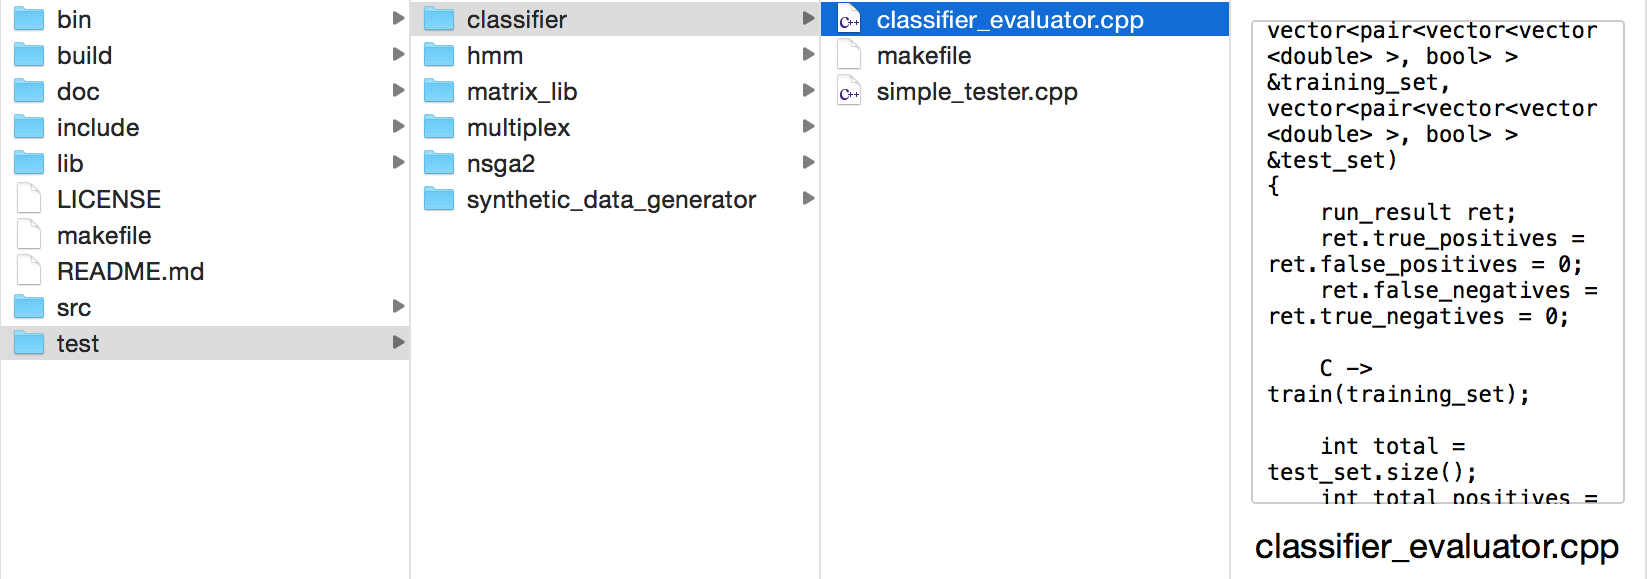
\includegraphics[width=0.9\textwidth]{figs/organisation}
	\caption[Overview of the project's source tree]{Overview of the project's source tree.}\label{figtree}
\end{figure}

\section{Summary}

This chapter has summarised the work I completed before the implementation phase of the project began; in particular, I have provided a review of the background theory underpinning the project (specifically, multiplex networks and hidden Markov models), and discussed the analysis of the project's requirements and deliverables, as well as the relevant tools and methodologies adopted.\\ \\
The next chapter will focus on the implementation of the project, giving details on how the proposed goals were actually achieved. 

\chapter{Implementation}

\emph{In this chapter, I will thoroughly describe the implementation phase of my project, resulting in successfully achieving the deliverables outlined in the Preparation chapter. This will follow the logical order of the implementation strategy adopted for the project---starting from the core project components, following up with a discussion of the extensions.\\ \\
The final implementation consists of over 5000 lines of \CC, and as such it is not suitable to showcase large code excerpts; rather, this chapter will focus on the high-level descriptions of the implemented algorithms (using pseudocode where appropriate), while larger code fragments will be confined to the appendices (ref. Appendix \ref{seccodesamples}.)}

\section{Overview}

The sections of the Implementation chapter will discuss the achievement of the deliverables related to the various models of machine learning that are capable of taking advantage of multiplexity, as outlined in \cref{secreq}. Initially, a brief overview of the \emph{supervised learning setup} (which is common to all of the implemented models) will be given in \cref{secsuplrn}; afterwards, the implementation of the models will be discussed in the following order:
\begin{enumerate}
	\item {\bf Multiplex chain GMHMM} (\cref{secmuxchngmhmm}): the simpler of the models, implementing a highly simplified GMHMM layer as its basis, to allow for easier implementation, suitable for the core deliverable. Its key components will be described in turn (\cref{seccgmhmm}--\ref{secmultiobj}).
	\item {\bf Full multiplex GMHMM} (\cref{secfullgmhmm}): once the core model is properly discussed, I will describe how to generalise it to utilise a completely flexible GMHMM in each layer of the multiplex network. As the model has many similarities to the chain version, only the most major difference (the training algorithm) will be discussed thoroughly (\cref{secbaumwelch}--\ref{secfulltrn}).
	%\item {\bf Aggregate multiplex model} (\cref{secaggr}): finally, I will describe a model that, unlike the previously mentioned models, does not rely on hidden Markov models; instead, this model focuses entirely on known multiplex network metrics for inference purposes.
\end{enumerate}

\section{Supervised learning setup}\label{secsuplrn}

All of the implemented machine learning models will be solving a \emph{supervised learning} \cite{mohri2012foundations} problem. This specifies the basic top-level interface that each model must expose, and hence is a logical place to initiate the discussion of the implementation phase.\\ \\
A model for the supervised learning problem aims to construct a \emph{labelling function}, $h : X \rightarrow Y$, to assign labels from a given set $Y$ to inputs from a set $X$. This function is constructed as the output of a \emph{learning algorithm}, $L : (X \times Y)^n \rightarrow (X \rightarrow Y)$, which attempts to generalise from a set of inputs with known labels---a \emph{training set}---to produce a function capable of labelling previously \emph{unseen} inputs. The process is summarised by the diagram given in Figure \ref{figsuplrn}.

\begin{figure}[H]
\centering
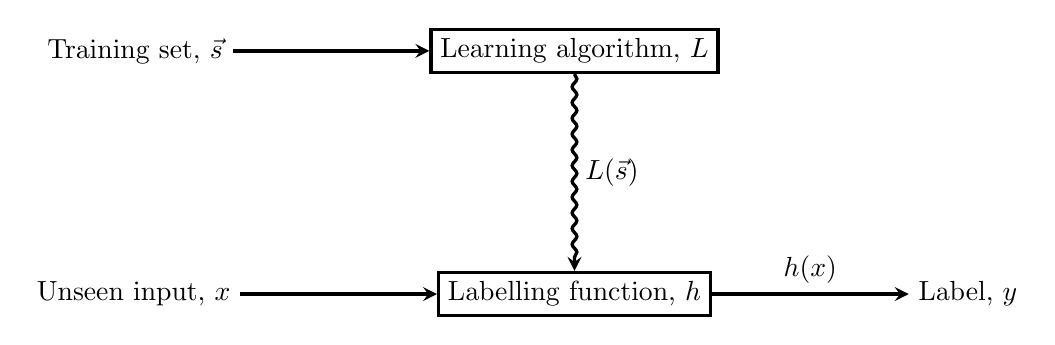
\begin{tikzpicture}[node distance=2.5cm]
	\node[rectangle, very thick, draw] (learning) {Learning algorithm, $L$};
	\node[rectangle, very thick, draw, below = of learning] (inference) {Labelling function, $h$};
	\node[left = of learning] (train) {Training set, $\vec{s}$};
	\node[left = of inference] (uns) {Unseen input, $x$};
	\node[right = of inference] (lab) {Label, $y$};
	
	\draw[-stealth, very thick] (train) -- (learning);
	\draw[-stealth, very thick, decoration={snake, segment length=2mm, amplitude=0.3mm, post length=1.5mm}, decorate] (learning) -- node[right] {$L(\vec{s})$} (inference);
	\draw[-stealth, very thick] (uns) -- (inference);
	\draw[-stealth, very thick] (inference) -- node[above] {$h(x)$} (lab);
\end{tikzpicture}
	\caption[Diagram of the supervised learning setup]{A diagram of the supervised learning setup.}\label{figsuplrn}
\end{figure}
\noindent As such, each of the models we consider has to provide an implementation of at least these two functions, \texttt{train($\overrightarrow{(X, Y)}$)} and \texttt{classify($X$)}.\\ \\
The statement of the primary problem (given in \cref{secreq}) specifies that $Y = \{C_1, C_2\}$ (binary classification), and also that $X = (\mathbb{R} \times \mathbb{R})^n$. However, for making the interface more easily extendable to other kinds of problems, it has been templated with the types corresponding to the sets $X$ and $Y$, as described in Listing \ref{lst:interface}; a typical model discussed within this project will extend from \texttt{Classifier<vector<vector<\textcolor{blue}{double}> >, \textcolor{blue}{bool}>}\footnote{{\bf N.B.} a \texttt{vector} was used for the second dimension rather than \texttt{pair}, to easily allow for using the structure with more than two types of data at once.}.
\begin{lstlisting}[caption={An interface for a classifier in the supervised learning setup.}, label={lst:interface}]
template<typename Data, typename Label>
class Classifier
{
public:
	virtual ~Classifier() { }
	virtual void train(std::vector<std::pair<Data, Label> > &training_set) = 0;
	virtual Label classify(Data &test_data) = 0;
};
\end{lstlisting}

\section{Multiplex chain GMHMM}\label{secmuxchngmhmm}

\subsection{Chain GMHMM}\label{seccgmhmm}

The simplest of the single-layer models considered is a GMHMM where all of the states are arranged in a \emph{chain-like structure} (as depicted in Figure \ref{figchngmm}). The model always starts in state $0$, with each state transitioning into the next one along the chain with probability $1$. Each state on the chain has its own probability distribution of the sub-outputs (represented in the form of the usual \emph{emission probability matrix}, ${\bf O'}$), and each sub-output stores its own parameters for the output's Gaussian distribution ($\mu, \sigma$).\\ \\
It is assumed that the amount of states in the chain is \textbf{equal} to the amount of outputs observed, that it is known which sub-output produced each output, and that the outputs can be ordered in some way; if they represent temporal data, then the ordering is trivial (sorted by time). Otherwise, a procedure should be first employed to sort the outputs in some sensible way (e.g. \cite{mouret2009classification}).
\begin{figure}[H]
\centering
%TC:ignore
\begin{tikzpicture} [scale = 1.3, every node/.style={transform shape},start chain=1 going right,
            					 start chain=2 going right]
            	%\draw[step=1cm,gray,very thin] (-2,-5) grid (6,5);
				\node[text depth=0pt] at (-2, 0) (S) {start};
				\node[state, on chain=1, very thick, text depth=0pt] (1) {$0$};
				\node[state, on chain=1, very thick, text depth=0pt] (2) {$1$};
				\node[state, on chain=1, very thick, text depth=0pt] (3) {$2$};
				\node[on chain=1] (md) {\dots};
				\node[state, on chain=1, very thick, text depth=0pt] (n) {$n$};
		 		\draw[>=stealth, very thick, auto=right,loop above/.style={out=75,in=105,loop}, every loop]
		 			(S) edge (1)
					(1) edge node[above] {$1$} (2)
					(2) edge node[above] {$1$} (3)
					(3) edge node[above] {$1$} (md)
					(md) edge node[above] {$1$} (n);
					
				\node[rectangle, thick, draw] at (-2, 1.7) (y1) {$id_0$};
				\node[rectangle, thick, draw] at (0, 1.7) (y2) {$id_1$};
				\node[rectangle, thick, draw] at (2, 1.7) (y3) {$id_2$};
				\node at (4, 1.7) (ymd) {\dots};
				\node[rectangle, thick, draw] at (6, 1.7) (yn) {$id_n$};
				
				\draw[-stealth, very thick, dashed]
					(1) edge node[right] {${\bf O'}_{0,id_0}$} (y1)
					(2) edge node[right] {${\bf O'}_{1,id_1}$} (y2)
					(3) edge node[right] {${\bf O'}_{2,id_2}$} (y3)
					(n) edge node[right] {${\bf O'}_{n,id_n}$} (yn);
					
				\node[rectangle, draw, scale=0.2, minimum size=20em,above = 2cm of y1] at (-1, 2) (gauss1) {\begin{tikzpicture}
\begin{axis}[axis lines=none, ticks=none,xmax=3, xmin=-3,ymax=1.1]
\addplot[ultra thick,black, no markers,samples=200] {exp(-x^2)};
\end{axis}\end{tikzpicture}};

				\node[rectangle, draw, scale=0.2, minimum size=20em,above = 2cm of y2] at (1, 2) (gauss2) {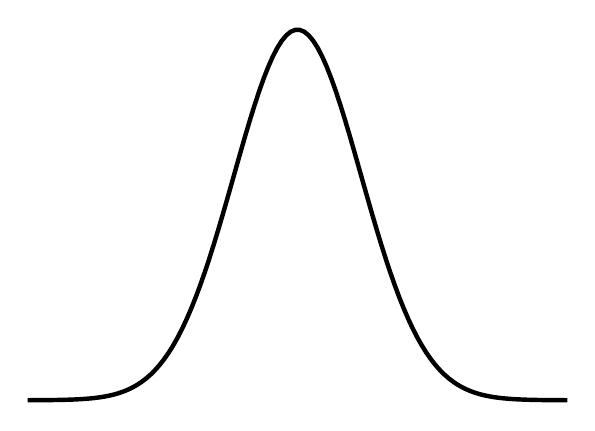
\begin{tikzpicture}
\begin{axis}[axis lines=none, ticks=none,xmax=3, xmin=-3,ymax=1.1]
\addplot[ultra thick,black, no markers,samples=200] {exp(-x^2)};
\end{axis}\end{tikzpicture}};

				\node[rectangle, draw, scale=0.2, minimum size=20em,above = 2cm of y3] at (3, 2) (gauss3) {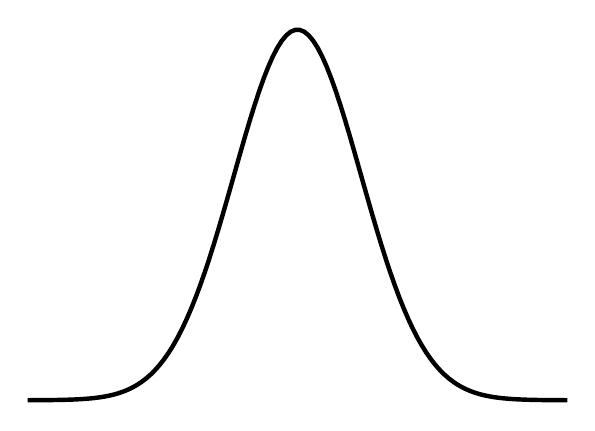
\begin{tikzpicture}
\begin{axis}[axis lines=none, ticks=none,xmax=3, xmin=-3,ymax=1.1]
\addplot[ultra thick,black, no markers,samples=200] {exp(-x^2)};
\end{axis}\end{tikzpicture}};
				
				\node at (5, 4.7) (gaussmd) {\dots};
				
				\node[rectangle, draw, scale=0.2, minimum size=20em,above = 2cm of yn] at (7, 2) (gaussn) {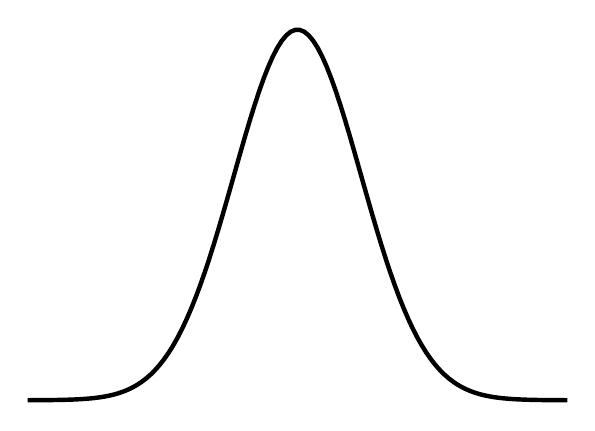
\begin{tikzpicture}
\begin{axis}[axis lines=none, ticks=none,xmax=3, xmin=-3,ymax=1.1]
\addplot[ultra thick,black, no markers,samples=200] {exp(-x^2)};
\end{axis}\end{tikzpicture}};
				
				\draw[-stealth, very thick, dotted]
					(y1) edge node[left] {$\mu_{id_0}$} node[right] {$\sigma_{id_0}$} (gauss1)
					(y2) edge node[left] {$\mu_{id_1}$} node[right] {$\sigma_{id_1}$} (gauss2)
					(y3) edge node[left] {$\mu_{id_2}$} node[right] {$\sigma_{id_2}$} (gauss3)
					(yn) edge node[left] {$\mu_{id_n}$} node[right] {$\sigma_{id_n}$} (gaussn);
			\end{tikzpicture}
%TC:endignore
	\caption[Example of a chain GMHMM]{\centering An example ``trace of execution'' of a chain GMHMM with $n+1$ states, with a sub-output sequence $\{id_i\}_{i=0}^n$.}\label{figchngmm}
\end{figure}
\noindent This is a very ``lightweight'' model, in the sense of the amount of data that needs to be stored to maintain it---as shown by Listing \ref{lst:chain}, only the amount of states and sub-outputs, the matrix ${\bf O'}$ and the parameters $\vec{\mu}$ and $\vec{\sigma}$ need to be maintained.
\begin{lstlisting}[caption={The state of a chain GMHMM.}, label={lst:chain}, float,floatplacement=H]
class SimpleChainGMHMM
{
private:
	int obs, sub_obs; // number of states and "sub-observations"
	double **G; // sub-observation emission probabilites
	double *mu, *sigma; // means and variances for each sub-observation
    
public:
	... // methods
};
\end{lstlisting}

\subsubsection{Output likelihood}\label{secoutlik}

The main building block for the inference algorithm for the chain GMHMM (and all of the other models that will be considered) is the method that determines the {\bf likelihood}, $\mathbb{L}(\vec{y}, \vec{id})$, of a given output sequence being produced by the model.\\ \\
Note the change in terminology; we are looking for the \emph{likelihood} rather than the \emph{probability} of the sequence being emitted. This is due to the fact that, in continuous space, the probability of any individual sequence being observed is zero. In the context of likelihood, we will use the \emph{Gaussian probability density function}, $\mathcal{N}(x; \mu, \sigma)$, instead of the actual probability, because what we are interested in is typically {\bf not} the actual likelihood, but rather \emph{how it compares to other likelihoods}.\\ \\
For a chain GMHMM $\bf \Theta$, the output likelihood is easily expressible as
\[\mathbb{L}(\vec{y}, \vec{id}|{\bf \Theta}) = \prod_{i=0}^{n}{{\bf O'}_{i, id_i} \mathcal{N}(y_i; \mu_{id_i}, \sigma_{id_i})}\]
i.e.\! the product of the probabilities of emitting each sub-output, multiplied with the likelihoods of emitting each output from its sub-output. However, a product of many such floating-point values, particularly if several of them are close to zero, is prone to underflow. As such, it is typically better to calculate the {\bf log-likelihood} instead:
\[\log{(\mathbb{L}(\vec{y}, \vec{id}|{\bf \Theta}))} = \sum_{i=0}^{n}{(\log{({\bf O'}_{i, id_i})} +  \log{(\mathcal{N}(y_i; \mu_{id_i}, \sigma_{id_i}))})}\]
This formula lends itself to a simple $O(n)$-time algorithm which simply sums up the relevant values.

\subsubsection{Parameter estimation}\label{secparest}

Training a chain GMHMM consists of estimating its state (${\bf O'}, \vec{\mu}, \vec{\sigma}$) from a set of output sequences presumed to be generated by the model. The implication of this is that the state should be chosen such that the likelihoods of the sequences being produced by the model are high, while still allowing for flexibility (i.e. not \emph{overfitting} the model).\\ \\
The parameters $\vec{\mu}$ and $\vec{\sigma}$ are easy to estimate; for a given sub-output $x$, we extract all of the $k$ given outputs produced by it, $\vec{o_x}$, and then use their \emph{sample mean} and \emph{corrected sample standard deviation} to estimate $\mu_x$ and $\sigma_x$:
\[\mu_x = \frac{1}{k}\sum_{i=1}^{k}{(o_x)_i}\]
\[\sigma_x = \sqrt{\frac{1}{k-1}\sum_{i=1}^{k}{((o_x)_i - \mu_x)^2}}\]
The estimation of ${\bf O'}$ is less straightforward, and a variety of schemes could be used. I devised a method that assigns to each field of the matrix a {\bf score}, with the scores being normalised for each row of the matrix in the end. A na\"ive scheme would simply increment the score of ${\bf O'}_{xy'}$ whenever the state $x$ produces the sub-output $y'$ in the training set, however this can lead to some suitable sequences being evaluated with the likelihood of zero---if they were to use an entry of the matrix that was never seen in the training data.\\ \\
To compensate for this, I devised a metric that ensures the following three features:
\begin{itemize}
	\item The na\"ive scheme's increments are still present; whenever state $x$ produces sub-output $y'$ in the training data, ${\bf O'}_{xy'} \leftarrow {\bf O'}_{xy'} + 1$.
	\item For each training sequence, each field of the matrix ${\bf O'}$ must be increased by {\bf at least} a given small, but manageable real number $\varepsilon$; within my project I set $\varepsilon = 10^{-6}$.
	\item For a given training sequence $s = (\vec{y}, \vec{id})$, a particular field ${\bf O'}_{xy'}$'s assigned score should {\bf decay exponentially} as $d_s(id_x, y')$, the \emph{distance} between $y'$ and the sub-output actually produced by $x$ ($id_x$), increases.
\end{itemize}
The choice of $d_s(id_x, y')$ is left to the user; a simple definition would be to take the smallest possible $|x - x'|$, where $x'$ is a state producing $y'$ in the given training sequence, along with a fixed value (perhaps $n+1$) if there is no such $x'$ in the sequence.\\ \\
With respect to the given features, a possible scoring function is
\[score_s(x, y') = e^{-\lambda d_s(id_x, y')}\]
where $\lambda = \frac{-\ln{\varepsilon}}{M}$, and $M$ is the \emph{maximal} observed value of $d_s(id_x, y')$ in the training set. A plot of this function is given in Figure \ref{figplot}; it clearly satisfies all of the desired properties.
\begin{figure}[H]
\centering
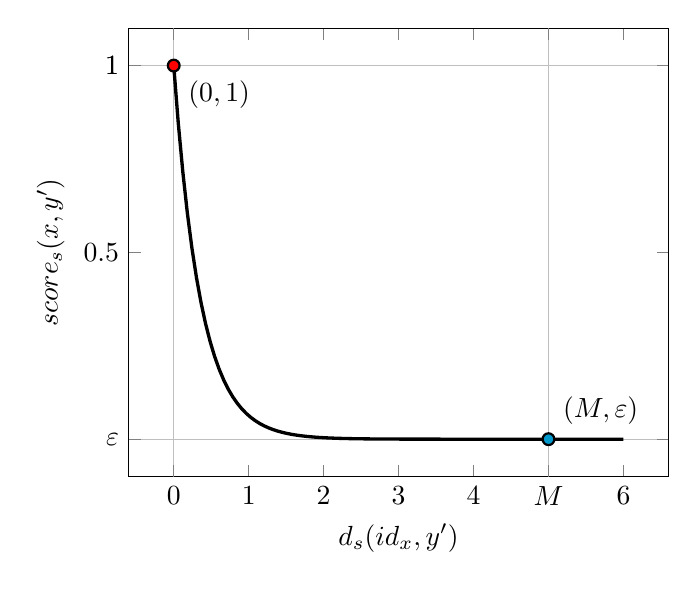
\begin{tikzpicture}
  \begin{axis}[
    xlabel={$d_s(id_x, y')$},
    ylabel={$score_s(x, y')$},
    ytick={0.5, 1},
    yticklabels={$0.5$, $1$},
    xtick={1,2,3,4,6},
    xticklabels={$1$,$2$,$3$,$4$,$6$},
    extra y ticks={0.000001, 1},
    extra y tick style={
        grid=major,
        yticklabels={$\varepsilon$, $1$},
        yticklabel style={anchor=east}},
    extra x ticks={0, 5},
    extra x tick style={
        grid=major,
        xticklabels={$0$, $M$},
        xticklabel style={anchor=north}}
  ]
    \addplot[color=black, very thick,domain=0:6, 
    samples=100] {exp(-2.7631*x)}; 
    \node[label={-45:{$(0, 1)$}},circle,draw=black, thick, fill=red,inner sep=1.5pt] at (axis cs:0, 1) {};
    \node[label={45:{$(M, \varepsilon)$}},draw=black, thick, circle,fill=echodrk,inner sep=1.5pt] at (axis cs:5,0.000001) {};
  \end{axis}
\end{tikzpicture}
	\caption[Plot of $score_s(x, y')$ as a function of $d_s(id_x, y')$]{A plot of $score_s(x, y')$ as a function of $d_s(id_x, y')$, given $M = 5$.}\label{figplot}
\end{figure}
\noindent Taking into account all of the above, Algorithm \ref{alg:parestg} represents the full training algorithm for a chain GMHMM. This algorithm has an asymptotic time complexity of $O(n\cdot m\cdot s)$ (dominated by the triply-nested {\tt for} loops), where $n$ is the number of states, $m$ is the number of sub-outputs, and $s$ is the number of training sequences in the set $\vec{s}$.

\begin{algorithm}
\caption{Chain GMHMM parameter estimation}\label{alg:parestg}
\begin{algorithmic}[1]
\Require{Chain GMHMM ${\bf \Theta} = (n, m, {\bf O'}, \vec{\mu}, \vec{\sigma})$, training set $\vec{s} = \overrightarrow{(\vec{y}, \vec{id})}$, distance function $d$, minimal score gain $\varepsilon$.}
\Procedure{TrainChn}{${\bf \Theta}$, ${\vec{s}}$, $d$, $\varepsilon$} \Comment{Estimate the parameters of ${\bf \Theta}$ using $\vec{s}$}
	\For{$y'\gets 0$ {\bf to} $m$} 
		\State $\vec{o_{y'}}\gets \emptyset$ \Comment{Initialise the sets of outputs for each sub-output}
		\State $k_{y'}\gets 0$
	\EndFor
	\State $M\gets 0$ \Comment{Initialise maximal distance observed}
	\ForAll{$s = (\vec{y}, \vec{id}) \in \vec{s}$}
		\For{$x\gets 0$ {\bf to} $n$}
			\For{$y'\gets 0$ {\bf to} $m$}
				\State $M\gets \max(M, d_s(id_x, y'))$ \Comment{Update maximal distance}
			\EndFor
			\State $\vec{o_{id_x}}$.\Call{PushBack}{$y_x$} \Comment{Fill the sets of outputs}
			\State $k_{id_x}\gets k_{id_x} + 1$
		\EndFor
	\EndFor
	\For{$y'\gets 0$ {\bf to} $m$} \Comment{Estimate $\vec{\mu}$ and $\vec{\sigma}$}
		\State \Call{Assert}{$k_{y'} > 1$} \Comment{\emph{Precondition:} Must have at least two outputs}
		\State $\mu_{y'}\gets\frac{1}{k_{y'}}\sum\limits_{i=1}^{k_{y'}}{(o_{y'})_i}$
		\State $\sigma_{y'}\gets \sqrt{\frac{1}{k_{y'}-1}\sum\limits_{i=1}^{k_{y'}}{((o_{y'})_i - \mu_{y'})^2}}$
	\EndFor
	\State $\lambda\gets\frac{-\ln{\varepsilon}}{M}$ \Comment{Set the $\lambda$ parameter used for $score_s$}
	\State ${\bf O'}\gets {\bf 0}_{(n+1)\times(m+1)}$ \Comment {Set the entries of ${\bf O'}$ to zero}
	\ForAll{$s = (\vec{y}, \vec{id}) \in \vec{s}$}
		\For{$x\gets 0$ {\bf to} $n$}
			\For{$y'\gets 0$ {\bf to} $m$}
				\State ${\bf O'}_{xy'}\gets {\bf O'}_{xy'} + score_s(x, y')$ \Comment{Assign score to each entry}
			\EndFor
		\EndFor
	\EndFor
	\For{$x\gets 0$ {\bf to} $n$}
		\State $S\gets \sum\limits_{y'=0}^{m}{{\bf O'}_{xy'}}$
		\For{$y'\gets 0$ {\bf to} $m$}
			\State ${\bf O'}_{xy'}\gets \frac{{\bf O'}_{xy'}}{S}$ \Comment{Normalise each row of the matrix}
		\EndFor
	\EndFor
\EndProcedure
\end{algorithmic}
\end{algorithm}

\subsubsection{Classifier construction}

Once the training procedure is properly defined, all of the elements needed for constructing a binary classifier using the chain GMHMM are in place:
\begin{itemize}
	\item[\tt train] This binary classifier, $C_{chain}$, will encapsulate {\bf two} chain GMHMMs, ${\bf \Theta_1}$ and ${\bf \Theta_2}$, one to be constructed using all the training sequences assigned to $C_1$, the other trained on all the sequences assigned to $C_2$ (Algorithm \ref{alg:trn}). 
	\item[\tt classify] Classifying an unseen sequence reduces to evaluating the (log-){\bf likelihoods} of the sequence being produced by \emph{each} of the two chain GMHMMs, choosing the class corresponding with the \emph{larger} likelihood (Algorithm \ref{alg:cls}). 
\end{itemize}
The same methodology will also be utilised in the other models discussed; as such, to define a new classifier from any model, it will be sufficient to specify the \emph{training} and \emph{likelihood} functions for the model.
\begin{algorithm}[H]
\caption{Chain GMHMM binary classifier: Training}\label{alg:trn}
\begin{algorithmic}[1]
\Require{Binary classifier $C_{chain} = ({\bf \Theta_1}, {\bf \Theta_2})$, two training sets of sequences $\vec{s_1}$ and $\vec{s_2}$, labelled with $C_1$ and $C_2$ respectively.}
\Procedure{Train}{$C_{chain}$, $\vec{s_1}$, $\vec{s_2}$} \Comment{Train the classifier using $\vec{s_1}$ and $\vec{s_2}$}
	\State \Call{TrainChn}{${\bf \Theta_1}$, $\vec{s_1}$, $d$, $10^{-6}$} \Comment{Train the first model using $\vec{s_1}$}
	\State \Call{TrainChn}{${\bf \Theta_2}$, $\vec{s_2}$, $d$, $10^{-6}$} \Comment{Train the second model using $\vec{s_2}$}
\EndProcedure
\end{algorithmic}
\end{algorithm}
\begin{algorithm}[H]
\caption{Chain GMHMM binary classifier: Classification}\label{alg:cls}
\begin{algorithmic}[1]
\Require{Binary classifier $C_{chain} = ({\bf \Theta_1}, {\bf \Theta_2})$, sequence $(\vec{y}, \vec{id})$ to be classified.}
\Function{Classify}{$C_{chain}$, $\vec{y}$, $\vec{id}$} \Comment{Classify $\vec{y}$ using $C_{chain}$}
	\State $\ell_1\gets$ \Call{LogLikelihood}{${\bf \Theta_1}$, $\vec{y}$, $\vec{id}$} \Comment{Get likelihood of $(\vec{y}, \vec{id})$ produced by ${\bf \Theta_1}$}
	\State $\ell_2\gets$ \Call{LogLikelihood}{${\bf \Theta_2}$, $\vec{y}$, $\vec{id}$} \Comment{Get likelihood of $(\vec{y}, \vec{id})$ produced by ${\bf \Theta_2}$}
	\If{$\ell_1 > \ell_2$} 
		\Return{$C_1$}\Comment{Return the class according to the likelihoods}
	\Else{} \Return{$C_2$}
	\EndIf
\EndFunction
\Ensure{The class that $(\vec{y}, \vec{id})$ belongs to, according to $C_{chain}$.}
\end{algorithmic}
\end{algorithm}

\subsection{Combining chains}

Now that the structure for classifying on a single type of data is fully specified, I will show how to extend it to a multiplex classifier operating on several data types simultaneously. In this subsection I will outline the parameters needed to specify the model, and give an algorithm for determining likelihoods of sequences being produced by it.

\subsubsection{Multiplex chain}\label{secmuxchaiin}

The chain GMHMM structure described thus far is very simple and not really a ``hidden'' Markov model, as the sequence of states it will take is \emph{pre-determined} by the parameters of the chain. This has been done to make \emph{combining} several chains as simple as possible.\\ \\
Assuming we have $L$ types of data in our output sequences, we may train $L$ separate chain GMHMMs; one on each of the types. Then, when producing any given sequence, we start in one of the chains, but \emph{allow the current chain to change} as we go along. This essentially means that the model will traverse along a chain as usual, but possibly change the type of data being used to produce the current full data point. \\ \\
The full structure should still represent an HMM, but now the starting state is no longer pre-determined; there are $L$ states responsible for processing the first data point. This requires the specification of a \emph{start-state probability vector}, $\vec{\pi}$, determining the probabilities of starting in each of the chains. Furthermore, we need to specify the probabilities of transitioning between each pair of chains; this may be conveniently represented as a matrix ${\boldsymbol \omega}$ of size $L \times L$, such that ${\boldsymbol \omega}_{ij}$ represents the probability of transitioning from chain $i$ to chain $j$ (or staying in chain $i$ if $i = j$; in fact, we may omit $\vec{\pi}$ if we set $\pi_i$ to be equal to the normalised entries of ${\boldsymbol \omega}_{ii}$). Observing the entire structure as an HMM, there is a transition from state $x$ in layer $i$ to state $x+1$ in layer $j$ with probability ${\boldsymbol \omega}_{ij}$. An example of a two-layer model is given in Figure \ref{figmuxchngm}\footnote{{\bf N.B.} this model does not fit the definition of a multiplex network as specified in \cref{secmuxnet}, as the network is not \emph{diagonally coupled}; however, it is possible to transform it into an equivalent multiplex network by \emph{adding more layers}.}.\\ \\
Most of the necessary information for specifying this model is already contained within the individual chains; as shown by Listing \ref{lst:muxchain}, along with the chains themselves, only the transition probability matrix, $\boldsymbol \omega$, and the amount of chains in the model, $L$, need to be stored (we may also store the number of states and sub-observations, for convenience).

\begin{lstlisting}[caption={The state of a multiplex chain GMHMM.}, label={lst:muxchain}, float, floatplacement=H]
class HMMChainMultiplex
{
private:
	int obs, sub_obs; // as before
	int L; // number of layers (data-types)
	std::vector<SimpleChainGMHMM*> layers; // chains
	double **omega; // transition probabilities
public:
	... // methods
};
\end{lstlisting}

\begin{figure}
	\centering
%TC:ignore 
	\begin{tikzpicture} [scale=1.3, every node/.style={transform shape},start chain=1 going right,
            					 start chain=2 going right]
        	%\draw[step=1cm,gray,very thin] (-2,-5) grid (6,5);
				\node[state, fill=red!20, on chain=1, very thick, text depth=0pt] (1) {$s_0$};
				\node[state, fill=red!20, on chain=1, very thick, text depth=0pt] (2) {$s_1$};
				\node[state, fill=red!20, on chain=1, very thick, text depth=0pt] (3) {$s_2$};
				\node[on chain=1] (md) {\dots};
				\node[state, fill=red!20, on chain=1, very thick, text depth=0pt] (n) {$s_n$};
		 		\draw[>=stealth, color=red, text=black, very thick, auto=right,loop above/.style={out=75,in=105,loop}, every loop]
					(1) edge node[above] {\footnotesize$\boldsymbol \omega_{11}$} (2)
					(2) edge node[above] {\footnotesize$\boldsymbol \omega_{11}$} (3)
					(3) edge node[above] {\footnotesize$\boldsymbol \omega_{11}$} (md)
					(md) edge node[above] {\footnotesize$\boldsymbol \omega_{11}$} (n);
					
				\node[rectangle, thick, fill=red!20, draw] at (-2, 1.7) (y1) {$id_0$};
				\node[rectangle, thick, fill=red!20, draw] at (0, 1.7) (y2) {$id_1$};
				\node[rectangle, thick, fill=red!20, draw] at (2, 1.7) (y3) {$id_2$};
				\node at (4, 1.7) (ymd) {\dots};
				\node[rectangle, thick, fill=red!20, draw] at (6, 1.7) (yn) {$id_n$};
				
				\draw[-stealth, color=red, text=black, very thick, dashed]
					(1) edge node[right] {${\bf O'}_{0,id_0}$} (y1)
					(2) edge node[right] {${\bf O'}_{1,id_1}$} (y2)
					(3) edge node[right] {${\bf O'}_{2,id_2}$} (y3)
					(n) edge node[right] {${\bf O'}_{n,id_n}$} (yn);
				
				\node[rectangle, fill=red!20, draw, scale=0.2, minimum size=20em,above = 2cm of y1] at (-1, 2) (gauss1) {\begin{tikzpicture}
\begin{axis}[axis lines=none, ticks=none,xmax=3, xmin=-3,ymax=1.1]
\addplot[ultra thick,black, no markers,samples=200] {exp(-x^2)};
\end{axis}\end{tikzpicture}};

				\node[rectangle, fill=red!20, draw, scale=0.2, minimum size=20em,above = 2cm of y2] at (1, 2) (gauss2) {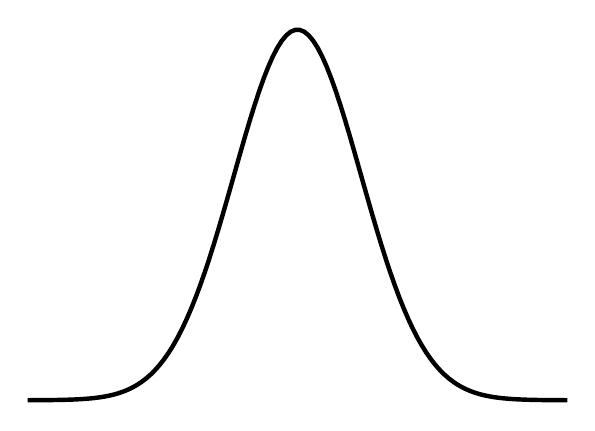
\begin{tikzpicture}
\begin{axis}[axis lines=none, ticks=none,xmax=3, xmin=-3,ymax=1.1]
\addplot[ultra thick,black, no markers,samples=200] {exp(-x^2)};
\end{axis}\end{tikzpicture}};

				\node[rectangle, fill=red!20, draw, scale=0.2, minimum size=20em,above = 2cm of y3] at (3, 2) (gauss3) {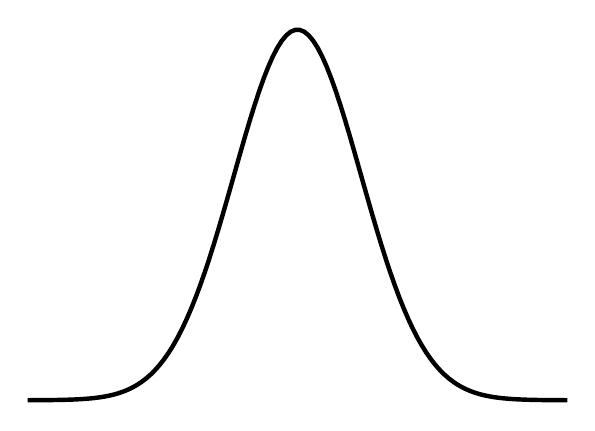
\begin{tikzpicture}
\begin{axis}[axis lines=none, ticks=none,xmax=3, xmin=-3,ymax=1.1]
\addplot[ultra thick,black, no markers,samples=200] {exp(-x^2)};
\end{axis}\end{tikzpicture}};
				
				\node at (5, 4.7) (gaussmd) {\dots};
				
				\node[rectangle, fill=red!20, draw, scale=0.2, minimum size=20em,above = 2cm of yn] at (7, 2) (gaussn) {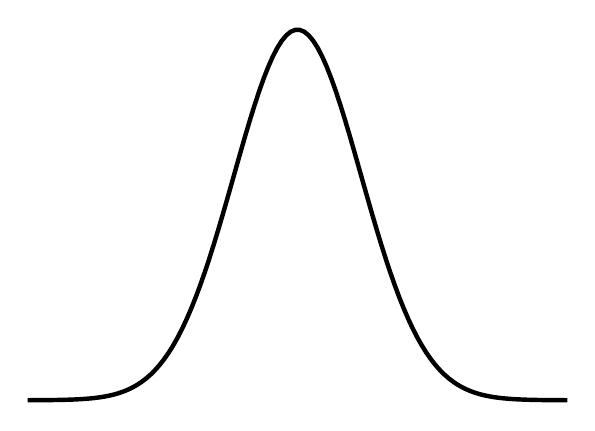
\begin{tikzpicture}
\begin{axis}[axis lines=none, ticks=none,xmax=3, xmin=-3,ymax=1.1]
\addplot[ultra thick,black, no markers,samples=200] {exp(-x^2)};
\end{axis}\end{tikzpicture}};
				
				\draw[-stealth, color=red, text=black, very thick, dotted]
					(y1) edge node[left] {$\mu_{id_0}$} node[right] {$\sigma_{id_0}$} (gauss1)
					(y2) edge node[left] {$\mu_{id_1}$} node[right] {$\sigma_{id_1}$} (gauss2)
					(y3) edge node[left] {$\mu_{id_2}$} node[right] {$\sigma_{id_2}$} (gauss3)
					(yn) edge node[left] {$\mu_{id_n}$} node[right] {$\sigma_{id_n}$} (gaussn);
				%%%%%% BOUNDARY %%%%%%%
					
				%%%%%% BOUNDARY %%%%%%%
				\node[state, fill=echodrk!20, on chain=2, very thick, text depth=0pt] (21) at (0, -2) {$s_0$};
				\node[state, fill=echodrk!20, on chain=2, very thick, text depth=0pt] (22) {$s_1$};
				\node[state, fill=echodrk!20, on chain=2, very thick, text depth=0pt] (23) {$s_2$};
				\node[on chain=2] (2md) {\dots};
				\node[state, fill=echodrk!20, on chain=2, very thick, text depth=0pt] (2n) {$s_n$};
		 		\draw[>=stealth, color=blue, text=black, very thick, auto=right,loop above/.style={out=75,in=105,loop}, every loop]
					(21) edge node[below] {\footnotesize$\boldsymbol \omega_{22}$} (22)
					(22) edge node[below] {\footnotesize$\boldsymbol \omega_{22}$} (23)
					(23) edge node[below] {\footnotesize$\boldsymbol \omega_{22}$} (2md)
					(2md) edge node[below] {\footnotesize$\boldsymbol \omega_{22}$} (2n);
					
				\node[rectangle, thick, fill=echodrk!20, draw] at (-2, -3.7) (2y1) {$id_0$};
				\node[rectangle, thick, fill=echodrk!20, draw] at (0, -3.7) (2y2) {$id_1$};
				\node[rectangle, thick, fill=echodrk!20, draw] at (2, -3.7) (2y3) {$id_2$};
				\node at (4, -3.7) (2ymd) {\dots};
				\node[rectangle, thick, fill=echodrk!20, draw] at (6, -3.7) (2yn) {$id_n$};
				
				\draw[-stealth, color=blue, text=black, very thick, dashed]
					(21) edge node[right] {${\bf O''}_{0,id_0}$} (2y1)
					(22) edge node[right] {${\bf O''}_{1,id_1}$} (2y2)
					(23) edge node[right] {${\bf O''}_{2,id_2}$} (2y3)
					(2n) edge node[right] {${\bf O''}_{n,id_n}$} (2yn);
				
				\node[rectangle, fill=echodrk!20, draw, scale=0.2, minimum size=20em,above = 2cm of 2y1] at (-1, -9.5) (2gauss1) {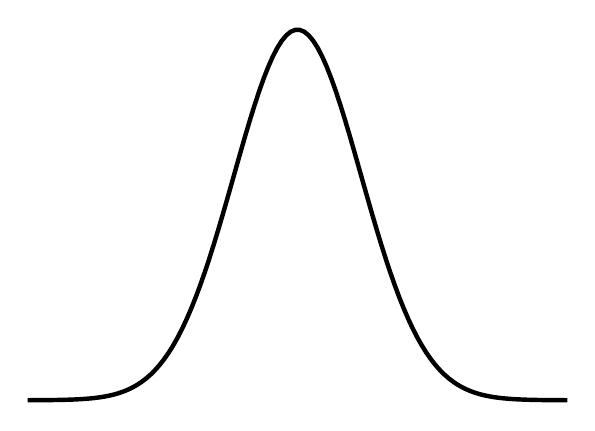
\begin{tikzpicture}
\begin{axis}[axis lines=none, ticks=none,xmax=3, xmin=-3,ymax=1.1]
\addplot[ultra thick,black, no markers,samples=200] {exp(-x^2)};
\end{axis}\end{tikzpicture}};

				\node[rectangle, fill=echodrk!20, draw, scale=0.2, minimum size=20em,above = 2cm of 2y2] at (1, -9.5) (2gauss2) {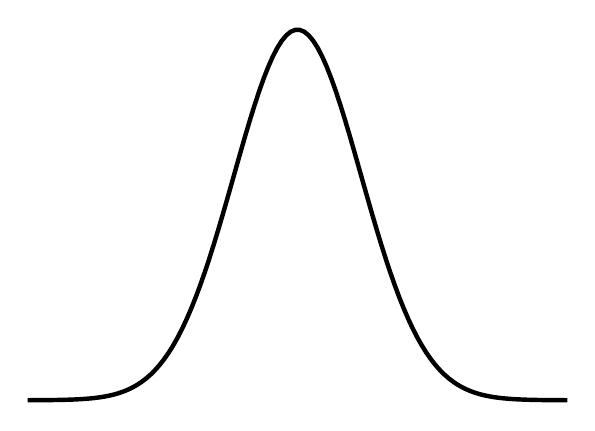
\begin{tikzpicture}
\begin{axis}[axis lines=none, ticks=none,xmax=3, xmin=-3,ymax=1.1]
\addplot[ultra thick,black, no markers,samples=200] {exp(-x^2)};
\end{axis}\end{tikzpicture}};

				\node[rectangle, fill=echodrk!20, draw, scale=0.2, minimum size=20em,above = 2cm of 2y3] at (3, -9.5) (2gauss3) {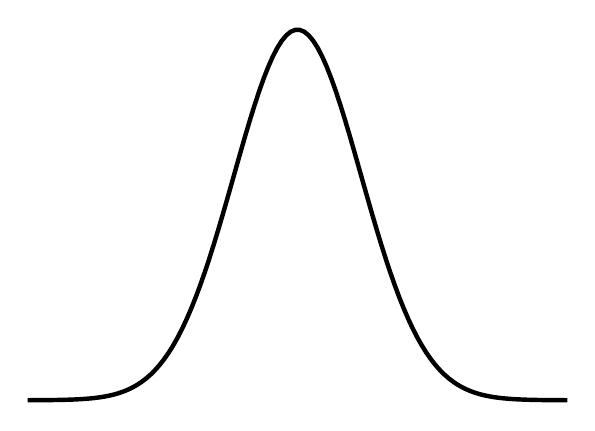
\begin{tikzpicture}
\begin{axis}[axis lines=none, ticks=none,xmax=3, xmin=-3,ymax=1.1]
\addplot[ultra thick,black, no markers,samples=200] {exp(-x^2)};
\end{axis}\end{tikzpicture}};
				
				\node at (5, -6.8) (2gaussmd) {\dots};
				
				\node[rectangle, fill=echodrk!20, draw, scale=0.2, minimum size=20em,above = 2cm of 2yn] at (7, -9.5) (2gaussn) {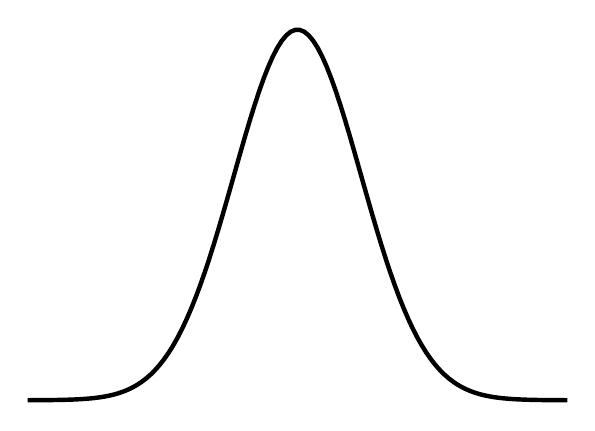
\begin{tikzpicture}
\begin{axis}[axis lines=none, ticks=none,xmax=3, xmin=-3,ymax=1.1]
\addplot[ultra thick,black, no markers,samples=200] {exp(-x^2)};
\end{axis}\end{tikzpicture}};
				
				\draw[-stealth, color=blue, text=black, very thick, dotted]
					(2y1) edge node[left] {$\mu'_{id_0}$} node[right] {$\sigma'_{id_0}$} (2gauss1)
					(2y2) edge node[left] {$\mu'_{id_1}$} node[right] {$\sigma'_{id_1}$} (2gauss2)
					(2y3) edge node[left] {$\mu'_{id_2}$} node[right] {$\sigma'_{id_2}$} (2gauss3)
					(2yn) edge node[left] {$\mu'_{id_n}$} node[right] {$\sigma'_{id_n}$} (2gaussn);	
					
				%%%% COMBO %%%%%
				\draw[-stealth, very thick, auto=right,decoration={snake, segment length=2mm, amplitude=0.5mm,post length=1.5mm}]
					(1) edge[decorate] node[left, near start] {\footnotesize$\boldsymbol \omega_{12}$} (22)
					(2) edge[decorate] node[left, near start] {\footnotesize$\boldsymbol \omega_{12}$} (23)
					(3) edge[decorate] node[left, near start] {\footnotesize$\boldsymbol \omega_{12}$} (2md)
					(md) edge[decorate] node[left, near start] {\footnotesize$\boldsymbol \omega_{12}$} (2n);
				\draw[-stealth, very thick, auto=right,decoration={snake, segment length=2mm, amplitude=0.5mm,post length=1.5mm}]
					(21) edge[decorate] node[left, near start] {\footnotesize$\boldsymbol \omega_{21}$} (2)
					(22) edge[decorate] node[left, near start] {\footnotesize$\boldsymbol \omega_{21}$} (3)
					(23) edge[decorate] node[left, near start] {\footnotesize$\boldsymbol \omega_{21}$} (md)
					(2md) edge[decorate] node[left, near start] {\footnotesize$\boldsymbol \omega_{21}$} (n);
				
				%%%% START STATES %%%%%
				\node[text depth=0pt] at (-2, -1) (S) {start};
				\draw[-stealth, very thick, auto=right,decoration={snake, segment length=2mm, amplitude=0.5mm,post length=1.5mm}]
					(S) edge[decorate] node[above] {\footnotesize$\pi_1$} (1)
					(S) edge[decorate] node[below] {\footnotesize$\pi_2$} (21);
	\end{tikzpicture}
%TC:endignore
	\caption[Example of a multiplex chain GMHMM]{Example of a multiplex chain GMHMM with two layers.}\label{figmuxchngm}
\end{figure}

\subsubsection{Forward algorithm}\label{secfwdalgs}

As the model can now be observed as a general hidden Markov model (not being known exactly which state sequence the model will follow), a new method for calculating likelihoods is needed; I will first introduce the solution for a generalised GMHMM, and then briefly discuss ways in which it could be optimised for the chain GMHMM.\\ \\
Given a GMHMM ${\bf \Theta} = (n, m, \vec{\pi}, {\bf T}, {\bf O'}, \vec{\mu}, \vec{\sigma})$, we may attempt to evaluate the likelihood of an output sequence similarly as in \cref{secoutlik}; assuming we have an output sequence $(\vec{y}, \vec{id})$ of length $T$, the total likelihood of the sequence being produced by the GMHMM may be evaluated by summing over all possible state sequences:
\[\mathbb{L}(\vec{y}, \vec{id}|{\bf \Theta}) = \sum_{\vec{x} \in S^T}\mathbb{L}(\vec{y}, \vec{id}|\vec{x}, {\bf \Theta})\mathbb{L}(\vec{x}|{\bf \Theta})\]
However, the number of possible state sequences is \emph{exponential} in $T$; hence this approach is infeasible. For a better approach, note that a lot of the calculations performed this way are redundant, and reusing previously calculated results can speed up the evaluation; this leads to a \emph{dynamic programming} algorithm known as the {\bf forward algorithm}.\\ \\
The forward algorithm computes \textbf{forward likelihoods}, $\alpha_t(x)$, corresponding to the likelihood of processing the first $t$ elements of the output sequence and ending up in state $x$:
\[\alpha_t(x) \myeq \mathbb{L}(\{(y_i, id_i)\}_{i=1}^t, x_t = x|{\bf \Theta})\]
Having computed all of the values of $\alpha_t(x)$, the overall likelihood may be evaluated as
\[\mathbb{L}(\vec{y}, \vec{id}|{\bf \Theta}) = \sum_{x \in S}\mathbb{L}(\vec{y}, \vec{id}, x_T = x|{\bf \Theta}) = \sum_{x \in S}\alpha_T(x)\]
The \emph{base cases}, $\alpha_1(x)$, can be simply computed as
\[\alpha_1(x) = \mathbb{L}((y_1, id_1), x_1 = x|{\bf \Theta}) = \pi_x{\bf O'}_{x,id_1}\mathcal{N}(y_1; \mu_{id_1}, \sigma_{id_1})\]
Assuming we have already computed $\alpha_t(x)$ for all $x$, we can derive an expression for $\alpha_{t+1}(x)$ as follows (the dependencies between the previously calculated likelihoods and the new one are illustrated in Figure \ref{figfwd}):
\[\begin{aligned}
\alpha_{t+1}(x) & = \mathbb{L}(\{(y_i, id_i)\}_{i=1}^{t+1}, x_{t+1} = x|{\bf \Theta})\\
& = \mathbb{L}((y_{t+1}, id_{t+1}) | x_{t+1} = x, \{(y_i, id_i)\}_{i=1}^{t}, {\bf \Theta})\mathbb{L}(\{(y_i, id_i)\}_{i=1}^{t}, x_{t+1} = x|{\bf \Theta})\\
& = \mathbb{L}((y_{t+1}, id_{t+1}) | x_{t+1} = x, {\bf \Theta})\sum_{x' \in S}{\mathbb{L}(\{(y_i, id_i)\}_{i=1}^{t}, x_{t+1} = x, x_t = x'|{\bf \Theta})}\\
& = {\bf O'}_{x,id_{t+1}}\mathcal{N}(y_{t+1}; \mu_{id_{t+1}}, \sigma_{id_{t+1}})\sum_{x' \in S}{\mathbb{L}(\{(y_i, id_i)\}_{i=1}^{t}, x_t = x'|{\bf \Theta})\mathbb{L}(x_{t+1} = x|x_t = x', {\bf \Theta})}\\
& = {\bf O'}_{x,id_{t+1}}\mathcal{N}(y_{t+1}; \mu_{id_{t+1}}, \sigma_{id_{t+1}})\sum_{x' \in S}{\alpha_t(x'){\bf T}_{x'x}}\\
\end{aligned}\]
This requires only $O(n)$ steps per state-time pair, and as such the overall time complexity of the forward algorithm is $O(n^2\cdot T)$.\\ \\
The forward algorithm is prone to the same underflow problems as the algorithm given in \cref{secoutlik}; however, as we are \emph{adding} components together instead of multiplying them, it is no longer suitable to trivially take the logarithm. A common solution is to normalise the entries of $\alpha_t(x)$ for each $t$, with a {\bf scaling coefficient} $c_t$:
\[c_t = \frac{1}{\sum\limits_{x\in S}{\alpha_t(x)}}\]
\begin{figure}[h]
\begin{center}
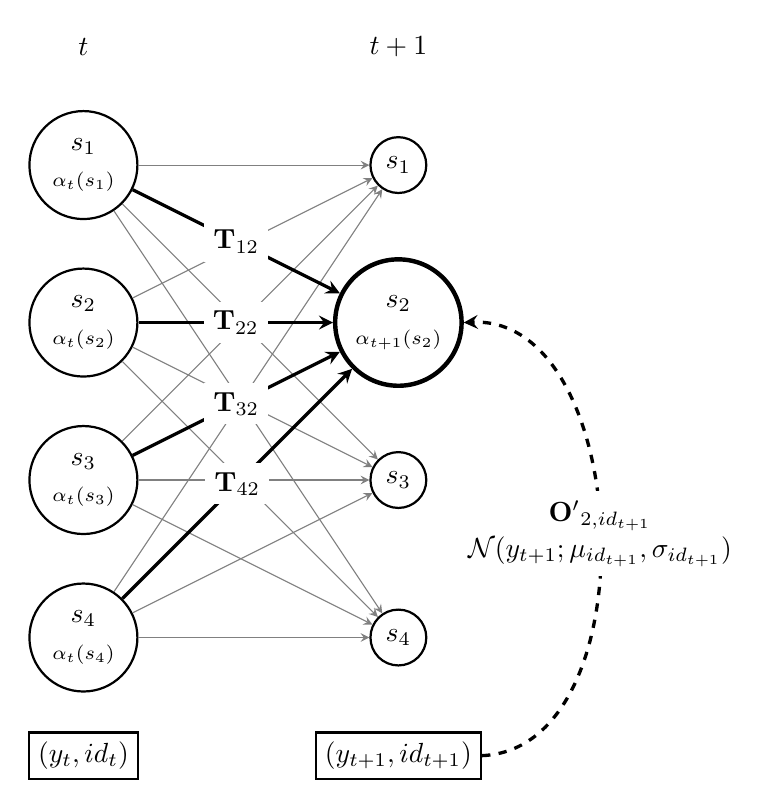
\begin{tikzpicture}[]
% 1st column
\node               at (0,6.5) {$t$};
\node[align=center, circle, draw, thick] (s1_1) at (0,5) {$s_1$\\{\scriptsize$\alpha_{t}(s_1)$}};
\node[align=center, circle, draw, thick] (s2_1) at (0,3) {$s_2$\\{\scriptsize$\alpha_{t}(s_2)$}};
\node[align=center, circle, draw, thick] (s3_1) at (0,1) {$s_3$\\{\scriptsize$\alpha_{t}(s_3)$}};
\node[align=center, circle, draw, thick] (s4_1) at (0,-1) {$s_4$\\{\scriptsize$\alpha_{t}(s_4)$}};
\node [draw, thick] at (0,-2.5) {$(y_t, id_t)$};
% 2nd column
\node               at (4,6.5) {$t+1$};
\node[circle, draw, thick] (s1_2) at (4,5) {$s_1$}
    edge[gray, thin, stealth-] (s1_1)
    edge[gray, thin, stealth-] (s2_1)
    edge[gray, thin, stealth-] (s3_1)
    edge[gray, thin, stealth-] (s4_1);
\node[circle, draw, thick] (s3_2) at (4,1) {$s_3$}
    edge[gray, thin, stealth-] (s1_1)
    edge[gray, thin, stealth-] (s2_1)
    edge[gray, thin, stealth-] (s3_1)
    edge[gray, thin, stealth-] (s4_1);
\node[circle, draw, thick] (s4_2) at (4,-1) {$s_4$}
    edge[gray, thin, stealth-] (s1_1)
    edge[gray, thin, stealth-] (s2_1)
    edge[gray, thin, stealth-] (s3_1)
    edge[gray, thin, stealth-] (s4_1);
\node[align=center, circle, draw, ultra thick] (s2_2) at (4,3) {$s_2$\\{\scriptsize$\alpha_{t+1}(s_2)$}};
\draw[very thick, stealth-]
    (s2_2) to node [midway, fill=white] {${\bf T}_{12}$} (s1_1);
\draw[very thick, stealth-]
    (s2_2) to node [midway, fill=white] {${\bf T}_{22}$} (s2_1);
\draw[very thick, stealth-]
    (s2_2) to node [midway, fill=white] {${\bf T}_{32}$} (s3_1);
\draw[very thick, stealth-]
    (s2_2) to node [midway, fill=white] {${\bf T}_{42}$} (s4_1);
\node [draw, thick] (asdf) at (4,-2.5) {$(y_{t+1}, id_{t+1})$};
\draw[-stealth, very thick, dashed, bend right=90] (asdf.east) to node[midway, align=center, fill=white] {${\bf O'}_{2,id_{t+1}}$\\$\mathcal{N}(y_{t+1};\mu_{id_{t+1}},\sigma_{id_{t+1}})$} (s2_2.east);
\end{tikzpicture}
\end{center}
\caption[Dependencies in the recurrence relation of the forward algorithm]{\centering Illustration of the recurrence relation of the forward algorithm on a GMHMM with four states; displaying all the variables that $\alpha_{t+1}(s_2)$ is dependent on.}\label{figfwd}
\end{figure}
The actual value of $\alpha_t(x)$ stored for future steps is
\[\hat{\alpha}_t(x) = c_t\alpha_t(x)\]
As the scaling coefficients propagate throughout the further calculations, the full likelihood of the sequence may be calculated as
\[\mathbb{L}(\vec{y}, \vec{id}|{\bf \Theta}) = \frac{\sum_{x \in S}\hat{\alpha}_T(x)}{c_1c_2\cdots c_T} = \prod_{t=1}^{T} \frac{1}{c_t}\]
the logarithm of which is easily maintainable as
\[\log{\mathbb{L}(\vec{y}, \vec{id}|{\bf \Theta})} = -\sum_{t=1}^{T} {\log{c_t}}\]
The pseudocode of the forward algorithm is given within Algorithm \ref{alg:fwd}. It could be optimised for the multiplex chain GMHMM by taking advantage of the fact that at time $t$ we may only be in state $t$, in one of the $L$ chains; as such, it suffices to store $\alpha_t(l)$, where $l$ ranges \emph{over all chains}; this reduces the time complexity to $O(L^2\cdot T)$.

\begin{algorithm}[H]
\caption{Forward algorithm}\label{alg:fwd}
\begin{algorithmic}[1]
\Require{GMHMM ${\bf \Theta} = (n, m, \vec{\pi}, {\bf T}, {\bf O'}, \vec{\mu}, \vec{\sigma})$, sequence $(\vec{y}, \vec{id})$ of length $T$.}
\Function{Forward}{${\bf \Theta}$, $\vec{y}$, $\vec{id}$, $T$} \Comment{Evaluate the likelihood $\mathbb{L}(\vec{y}, \vec{id}|{\bf \Theta})$}
	\For{$x\gets 1$ {\bf to} $n$}
		\State $\alpha_1(x)\gets\pi_x{\bf O'}_{x,id_1}\mathcal{N}(y_1; \mu_{id_1}, \sigma_{id_1})$ \Comment{Base cases; $\alpha_1(x)$}
	\EndFor
	\State $c_1\gets \frac{1}{\sum\limits_{x = 1}^{n}{\alpha_1(x)}}$ \Comment{Calculate the scaling coefficient}
	\For{$x\gets 1$ {\bf to} $n$}
		\State $\alpha_1(x)\gets c_1\alpha_1(x)$ \Comment{Normalise the entries}
	\EndFor
	\For{$t\gets 2$ {\bf to} $T$}
		\For{$x\gets 1$ {\bf to} $n$} \Comment{Recurrence relation for $\alpha_t(x)$}
			\State $\alpha_t(x)\gets{\bf O'}_{x,id_{t}}\mathcal{N}(y_{t}; \mu_{id_{t}}, \sigma_{id_{t}})\sum\limits_{x'=1}^{n}{\alpha_{t-1}(x'){\bf T}_{x'x}}$
		\EndFor
		\State $c_t\gets \frac{1}{\sum\limits_{x=1}^{n}{\alpha_t(x)}}$ \Comment{Calculate the scaling coefficient}
		\For{$x\gets 1$ {\bf to} $n$}
			\State $\alpha_t(x)\gets c_t\alpha_t(x)$ \Comment{Normalise the entries}
		\EndFor
	\EndFor
	\State $\ell\gets -\sum\limits_{t=1}^{n}{\log{c_t}}$ \Comment{Calculate the log-likelihood}
	\State \Return{$(\alpha, \vec{c}, \ell)$}
\EndFunction
\Ensure{The forward likelihoods $\alpha_t(x)$, the scaling coefficients $\vec{c}$, the log-likelihood $\ell$.}
\end{algorithmic}
\end{algorithm}

\subsection{Multiplex training}\label{secmultiobj}

With an algorithm for evaluating likelihoods in place, the only remaining component that needs to be specified for the multiplex chain GMHMM classifier to be constructed is the \emph{training algorithm}. As previously specified, the individual chains within the multiplex may be trained with the parameter estimation method defined in \cref{secparest}; once this is done, estimating the optimal interlayer transition probabilities ($\boldsymbol\omega$) remains. In this subsection I will introduce the optimisation algorithm that was chosen for this purpose; afterwards I will briefly discuss the integration of this algorithm with the multiplex network structure, in order to round off the training algorithm for the core model.

\subsubsection{Multiobjective optimisation}

As mentioned in \cref{secparest}, the model parameters we are aiming to obtain upon training should optimise the likelihoods of the sequences within the training set being produced, while still maintaining a level of flexibility.\\ \\
At the most essential level, we would like to optimise all of the likelihoods \emph{independently} of one another; this corresponds to a {\bf multiobjective optimisation problem}; for a given training set of $k$ sequences, $\vec{s}$, we would like to maximise, for a given (partially-trained) multiplex chain GMHMM $\bf \Theta$, the sequence of functions $\{f_i(\boldsymbol\omega)\}_{i=1}^{k}$, defined as the likelihoods of each of the sequences in the training set being produced by the model, assuming the interlayer transition probabilities are $\boldsymbol \omega$, i.e.
\[f_i(\boldsymbol \omega) = \mathbb{L}(s_i | \bf \Theta, \boldsymbol\omega)\]
In the typical case, it is unlikely that all of the functions will reach their global maxima simultaneously at the same $\boldsymbol\omega$; rather, a \emph{frontier} (the {\bf Pareto front}) will be reached, consisting of a set of points where it is impossible to further optimise one function without degrading at least one of the others---refer to Figure \ref{figparetoplot}. Formally, we say that a solution $\boldsymbol \omega$ {\bf dominates} solution $\boldsymbol \omega'$, denoted $\bomega \succ \bomega'$, if
\begin{enumerate}
	\item $\forall i.\ f_i(\bomega) \geq f_i(\bomega')$
	\item $\exists j.\ f_j(\bomega) > f_j(\bomega')$
\end{enumerate}
A solution $\bomega^*$ is \textbf{on the Pareto front} if there is \emph{no other solution that dominates it}. Within the context of multiobjective optimisation, all of the solutions on the Pareto front are treated as \emph{equally satisfactory}, and the aim of multiobjective optimisation algorithms is typically to extract as many points on the front as possible (preferably well-spread). The following part will discuss one such algorithm, which has been utilised for my project.
\begin{figure}[H]
\centering
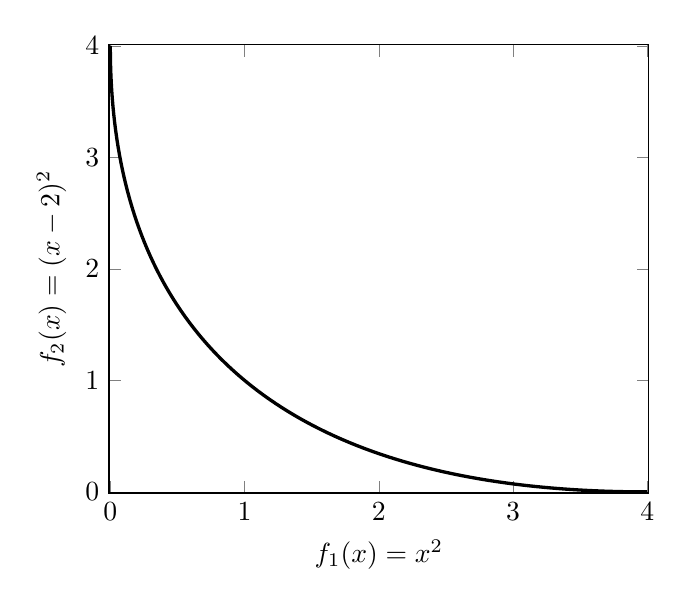
\begin{tikzpicture}
  \begin{axis}[
    xlabel={$f_1(x) = x^2$},
    ylabel={$f_2(x) = (x-2)^2$},
    xmin=-0.01, xmax = 4.01,
    ymin=-0.01, ymax = 4.01,
  ]
    \addplot[color=black, very thick,domain=0:2, 
    samples=100] ({x^2},{(x-2)^2});
  \end{axis}
\end{tikzpicture}
	\caption[Example of a Pareto front]{\centering The Pareto front for minimising the functions $f_1(x) = x^2$ and $f_2(x)=(x-2)^2$; obtained when $x\in [0, 2]$.}\label{figparetoplot}
\end{figure}
\noindent Arguably, we could find a way to combine the likelihoods in a single function to be optimised (making the approach simpler and only extracting a single point), however, vital information about the model is potentially lost this way; in my project I have opted for the multiobjective approach to allow the user to manually discriminate which points on the frontier are more favourable, using a method of their own choosing.

\subsubsection{NSGA-II}

A popular class of algorithms for solving the multiobjective optimisation problem are \emph{evolutionary algorithms}---population-based heuristics inspired by evolutionary concepts such as natural selection \cite{back1996evolutionary}. They are a good choice for a generalised optimisation problem as they \emph{make no assumptions} about the solution space. The algorithms usually operate by \emph{generating} a random initial population of solutions, \emph{selecting} the best-fit group of solutions, and then \emph{combining} them in some way, producing a set of new solutions to replace the less fit ones. The process of selecting and combining is \emph{repeated} until the desired level of convergence is achieved.\\ \\
One such algorithm is the \textbf{nondominated sorting genetic algorithm II} (\emph{NSGA-II}) by Deb \emph{et al.} \cite{deb2002fast}. It is a popular option because it usually provides a larger spread of solutions on the Pareto front and converges faster compared to similar evolutionary algorithms. Therefore, I decided to implement it for my project; this paragraph provides a summary of the algorithm.\\ \\
The algorithm starts by randomly generating a set of $n$ solutions, $P_0$, and combining them (in ways that will be discussed ahead) to obtain a set of $n$ additional solutions, $Q_0$. Assuming we have a set of solutions $R_t = P_t \cup Q_t$, one iteration of NSGA-II aims to produce from it a set of more fit solutions, $R_{t+1}$. The first stage of the iteration is \emph{selection}; selecting the $n$ most fit solutions to represent the set $P_{t+1}$.\\ \\
The primary criterion for fitness is given by \emph{nondominated sorting}, i.e.\!\!\! sorting solutions by the $\succ$ ordering. This can be efficiently performed by, for each solution $p \in R_t$, keeping track of the set of solutions it dominates, $S_p$, and number of solutions dominating it, $n_p$. All solutions $p$ with $n_p = 0$ constitute the \emph{first nondominated front}, $\mathcal{F}_1$ and will be added to $P_{t+1}$ first. Whenever a solution $p$ is added to a nondominated front $\mathcal{F}_i$, for every $q \in S_p$, $n_q$ is decremented; if $n_q = 0$, $q$ will be a member of the next nondominated front ($\mathcal{F}_{i+1}$). This procedure is repeated until every solution has been assigned to a front.\\ \\
The pseudocode is summarised in Algorithm \ref{alg:nondom}, and a visualisation of its output is given in Figure \ref{figfront}. Each pair of solutions is compared by $\succ$ exactly once, and a single such comparison takes $O(m)$ steps, where $m$ is the number of functions to optimise. After this phase, each pair of points is considered at most once while determining the nondominated fronts. As such, the initial comparisons dominate the running time of the algorithm, and hence its overall time complexity is $O(m\cdot n^2)$. The algorithm's space complexity is $O(n^2)$ (for storing the sets $S_p$).
\begin{algorithm}[H]
\caption{Fast nondominated sorting}\label{alg:nondom}
\begin{algorithmic}[1]
\Require{A set of solutions, $P$, to sort.}
\Function{FastNondominatedSort}{$P$} \Comment{Sort the elements of $P$ by $\succ$}
	\State $\vec{\mathcal{F}}\gets \emptyset$ \Comment{Initialise the nondominated fronts}
	\ForAll{$p \in P$}
		\State $S_p\gets\emptyset$ \Comment{Initialise $S_p$ and $n_p$}
		\State $n_p\gets 0$
		\ForAll{$q \in P$}
			\If{$p \succ q$} $S_p\gets S_p\cup \{q\}$ \Comment{Update $S_p$ or $n_p$}
			\ElsIf{$p \prec q$} $n_p\gets n_p + 1$
			\EndIf
		\EndFor
		\If{$n_p = 0$} $\mathcal{F}_1\gets\mathcal{F}_1\cup \{p\}$ \Comment{If no solution dominates $p$, $p$ is on $\mathcal{F}_1$}
		\EndIf
	\EndFor
	\State $i\gets 1$
	\While{$\mathcal{F}_i \neq \emptyset$} \Comment{Repeat until every solution has been assigned to a front}
		\ForAll{$p\in\mathcal{F}_i$}
			\ForAll{$q\in S_p$}
				\State $n_q\gets n_q - 1$ \Comment{$q$ has one solution less dominating it}
				\If{$n_q = 0$} $\mathcal{F}_{i+1}\gets \mathcal{F}_{i+1}\cup\{q\}$
				\EndIf
			\EndFor
		\EndFor
		\State $i\gets i+1$
	\EndWhile
	\State \Return{$\vec{\mathcal{F}}$}
\EndFunction
\Ensure{The nondominated fronts of $P$, $\vec{\mathcal{F}}$.}
\end{algorithmic}
\end{algorithm}
\begin{figure}[H]
\centering
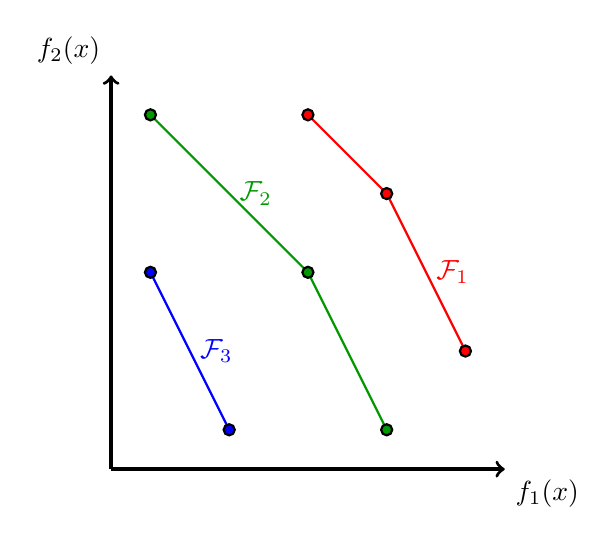
\begin{tikzpicture}

\draw[very thick,->] (0,0) -- (5,0) node[anchor=north west] {$f_1(x)$}; 
\draw[very thick,->] (0,0) -- (0,5) node[anchor=south east] {$f_2(x)$};


\draw[red, thick] (2.5, 4.5) -- (3.5, 3.5);
\draw[red, thick] (3.5, 3.5) -- node[right]{$\mathcal{F}_1$} (4.5, 1.5);
\draw[mygreen, thick] (0.5, 4.5) -- node[right]{$\mathcal{F}_2$} (2.5, 2.5);
\draw[mygreen, thick] (2.5, 2.5) -- (3.5, 0.5);
\draw[blue, thick] (0.5, 2.5) -- node[right]{$\mathcal{F}_3$} (1.5, 0.5);

\draw[fill=mygreen, thick] (2.5,2.5) circle (2pt) ;
\draw[fill=red, thick] (4.5,1.5) circle (2pt) ;
\draw[fill=mygreen, thick] (0.5,4.5) circle (2pt) ;
\draw[fill=mygreen, thick] (3.5,0.5) circle (2pt) ;
\draw[fill=blue, thick] (0.5,2.5) circle (2pt) ;
\draw[fill=blue, thick] (1.5,0.5) circle (2pt) ;
\draw[fill=red, thick] (3.5,3.5) circle (2pt) ;
\draw[fill=red, thick] (2.5,4.5) circle (2pt) ;

\end{tikzpicture}
\caption[Example output of nondominated sorting]{Example output of nondominated sorting; lines are drawn for clarity.}\label{figfront}	
\end{figure}

\noindent Usually, the final front that is to be added to $P_{t+1}$ cannot fit entirely; as such, we must further discriminate the solutions within that front. In this stage, the \emph{diversity} of the solutions is considered; this is done by evaluating the \emph{crowding-distance} parameter for each solution. For each function to be optimised, the crowding distance of each solution is increased by the difference between its immediate predecessor and successor by that function's value (specially, the endpoints are given a crowding distance of $+\infty$). The procedure is outlined in Algorithm \ref{alg:crowdist}; its time complexity is $O(m\cdot n \log{n})$ (dominated by sorting). For a visualisation of the crowding distance in 2D space, refer to Figure \ref{figcuboid}.
\begin{algorithm}[H]
\caption{Crowding distance assignment}\label{alg:crowdist}
\begin{algorithmic}[1]
\Require{A nondominated front of solutions, $\mathcal{I}$.}
\Procedure{CrowdingDistanceAssignment}{$\mathcal{I}$} \Comment{Assign crowding distances to $\mathcal{I}$}
	\State $l\gets |\mathcal{I}|$ \Comment{The number of solutions in the front}
	\For{$i\gets 1$ {\bf to} $l$} $\mathcal{I}_i.d\gets 0$ \Comment{Initialise crowding distances}
	\EndFor
	\ForAll{$f$ to optimise}
		\State \Call{Sort}{$\mathcal{I}$, $f$} \Comment{Sort the elements of $\mathcal{I}$ by the values of $f$}
		\State {$\mathcal{I}_1.d \gets \mathcal{I}_l.d \gets +\infty$} \Comment{Ensure that the endpoints are always preferred}
		\For{$i\gets 2$ {\bf to} $l-1$} \Comment{Increase the crowding distance for all other points}
			\State {$\mathcal{I}_i.d \gets \mathcal{I}_i.d + (\mathcal{I}_{i+1}.f - \mathcal{I}_{i-1}.f)$}
		\EndFor
	\EndFor
\EndProcedure
\end{algorithmic}
\end{algorithm}

\noindent Note that this, in combination with the previously defined $\succ$ relation, defines a new partial order, $\succ_n$ (the \emph{crowded-comparison} relation), as follows:
\[p\succ_n q \iff (p \succ q) \vee (p \nprec q \wedge p.d > q.d)\]
i.e. within a single nondominated front, the solutions that are \emph{further} away from their immediate neighbours are preferred.
\begin{figure}[H]
\centering
\begin{tikzpicture}

\draw[very thick,->] (0,0) -- (5,0) node[anchor=north west] {$f_1(x)$}; 
\draw[very thick,->] (0,0) -- (0,5) node[anchor=south east] {$f_2(x)$};

\draw[fill=black, thick] (0.5,4.5) circle (2pt) ;
\draw[fill=black, thick] (1.5,3.6) circle (2pt) node[above] {$i-1$};
\draw[fill=black, thick] (2.7,2.5) circle (2pt) node[above] {$i$};
\draw[fill=black, thick] (3.2,2.2) circle (2pt) node[below] {$i+1$};
\draw[fill=black, thick] (3.7,0.5) circle (2pt) ;
\draw[fill=light-gray, thick] (4.5,1.5) circle (2pt) ;
\draw[fill=light-gray, thick] (0.5,2.5) circle (2pt) ;
\draw[fill=light-gray, thick] (1.5,0.5) circle (2pt) ;
\draw[fill=light-gray, thick] (3.5,3.5) circle (2pt) ;
\draw[fill=light-gray, thick] (2.5,4.5) circle (2pt) ;

\draw[dashed] (1.5, 3.6) -- (1.5, 2.2);
\draw[dashed] (1.5, 2.2) -- (3.2, 2.2);

\end{tikzpicture}
\caption[Example of crowding distance]{\centering Example of crowding distance; for solution $i$ it corresponds to the length of the dashed line.}\label{figcuboid}	
\end{figure}
\noindent Once $P_{t+1}$ is produced, the next step is \emph{combining} its elements to produce $Q_{t+1}$. This is done by a \emph{randomised binary tournament} strategy:
\begin{enumerate}
	\item Two pairs of indices $(i, j)$ and $(k, l)$ are picked uniformly at random, each index from the range $[1, n]$;
	\item Solutions $p$ and $q$ are picked such that:
	\begin{enumerate}
		\item $p = \begin{cases}(P_{t+1})_i & (P_{t+1})_i \succ_n (P_{t+1})_j\\(P_{t+1})_j & \text{otherwise}\end{cases}$
		\item $q = \begin{cases}(P_{t+1})_k & (P_{t+1})_k \succ_n (P_{t+1})_l\\(P_{t+1})_l & \text{otherwise}\end{cases}$
	\end{enumerate}
	\item New solutions $p'$ and $q'$ are produced from $p$ and $q$ using the methods of \emph{crossover} and \emph{mutation}; these solutions are then added to $Q_{t+1}$.
	\item The algorithm is repeated until $n$ solutions have been produced.
\end{enumerate}
There are many ways of performing crossover and mutation; NSGA-II utilises \emph{simulated binary crossover (SBX)} and \emph{polynomial mutation} \cite{deb1994simulated}. As several parameters need to be introduced to properly define these operators, their respective formulae are omitted from this section; they may be found in Appendix \ref{secsbx}.\\ \\
The combining algorithm is outlined in Algorithm \ref{alg:comb}, and, as this is the final building block, the full NSGA-II pseudocode is given in Algorithm \ref{alg:nsga}. Its time complexity is dominated by the nondominated sorting subroutine, and as such it is $O(m\cdot n^2)$.
\begin{algorithm}[H]
\caption{Solution combining algorithm}\label{alg:comb}
\begin{algorithmic}[1]
\Require{A set of solutions, $P$.}
\Function{MakeNewPopulation}{$P$} \Comment{Generate a set of solutions $Q$, from $P$}
	\For{$x\gets 1$ {\bf to} $\frac{n}{2}$} 
		\State $i, j, k, l\gets$ \Call{Random}{$[1, n]$} \Comment{Choose competitors uniformly at random}
		\If{$P_i \succ_n P_j$} $p\gets P_i$ \Comment{Choose the first parent solution}
		\Else{} $p\gets P_j$
		\EndIf
		\If{$P_k \succ_n P_l$} $q\gets P_k$ \Comment{Choose the second parent solution}
		\Else{} $q\gets P_l$
		\EndIf
		\State $(p', q')\gets$ \Call{Crossover}{$p$, $q$} \Comment{Derive two child solutions via crossover}
		\State \Call{Mutate}{$p'$} \Comment{Mutate the child solutions}
		\State \Call{Mutate}{$q'$}
		\State $Q\gets Q\cup\{p', q'\}$ \Comment{Add the child solutions to the set $Q$}
	\EndFor
	\State \Return{$Q$}
\EndFunction
\Ensure{The set of new solutions, $Q$.}
\end{algorithmic}
\end{algorithm}

\begin{algorithm}[H]
\caption{NSGA-II}\label{alg:nsga}
\begin{algorithmic}[1]
\Require{A sequence of functions, $\{f_i\}_{i=1}^{m}$, to optimise, population size $n$, number of iterations $iter$.}
\Function{NSGA-II}{$\vec{f}$, $n$, $iter$} \Comment{Optimise the given set of functions}
	\State $P_0\gets$ \Call{Generate}{$n$} \Comment{Generate $n$ solutions uniformly at random}
	\State $Q_0\gets$ \Call{MakeNewPopulation}{$P_0$} \Comment{Generate $n$ child solutions}
	\For{$t\gets 0$ {\bf to} $iter-1$} 
		\State $R_t\gets P_t\cup Q_t$ \Comment{Combine parent and children solutions}
		\State $\vec{\mathcal{F}}\gets$ \Call{FastNondominatedSort}{$R_t$} \Comment{Find the nondominated fronts}
		\State $P_{t+1}\gets\emptyset$ \Comment{Initialise the next parent solution set}
		\State $i\gets 1$
		\While{$|P_{t+1}| + |\mathcal{F}_i| \leq n$} \Comment{Front $\mathcal{F}_i$ fits completely in the next set}
			\State \Call{CrowdingDistanceAssignment}{$\mathcal{F}_i$} \Comment{Calculate crowding distances}
			\State $P_{t+1}\gets P_{t+1}\cup \mathcal{F}_i$ \Comment{Add the front to the parent solution set}
			\State $i\gets i + 1$
		\EndWhile
		\State \Call{CrowdingDistanceAssignment}{$\mathcal{F}_i$} \Comment{Calculate crowding distances}
		\State \Call{Sort}{$\mathcal{F}_i$, $\succ_n$} \Comment{Sort the final front by the crowded-comparison relation}
		\State $P_{t+1}\gets P_{t+1}\cup\mathcal{F}_i[1..(n - |P_{t+1}|)]$ \Comment{Fill the remainder of the parent set}
		\State $Q_{t+1}\gets$ \Call{MakeNewPopulation}{$P_{t+1}$} \Comment{Generate $n$ child solutions}
	\EndFor
	\State \Return{$P_{iter}\cup Q_{iter}$} 
\EndFunction
\Ensure{The solution set obtained after $iter$ iterations, $P_{iter}\cup Q_{iter}$.}
\end{algorithmic}
\end{algorithm}
\begin{figure}[H]
\centering
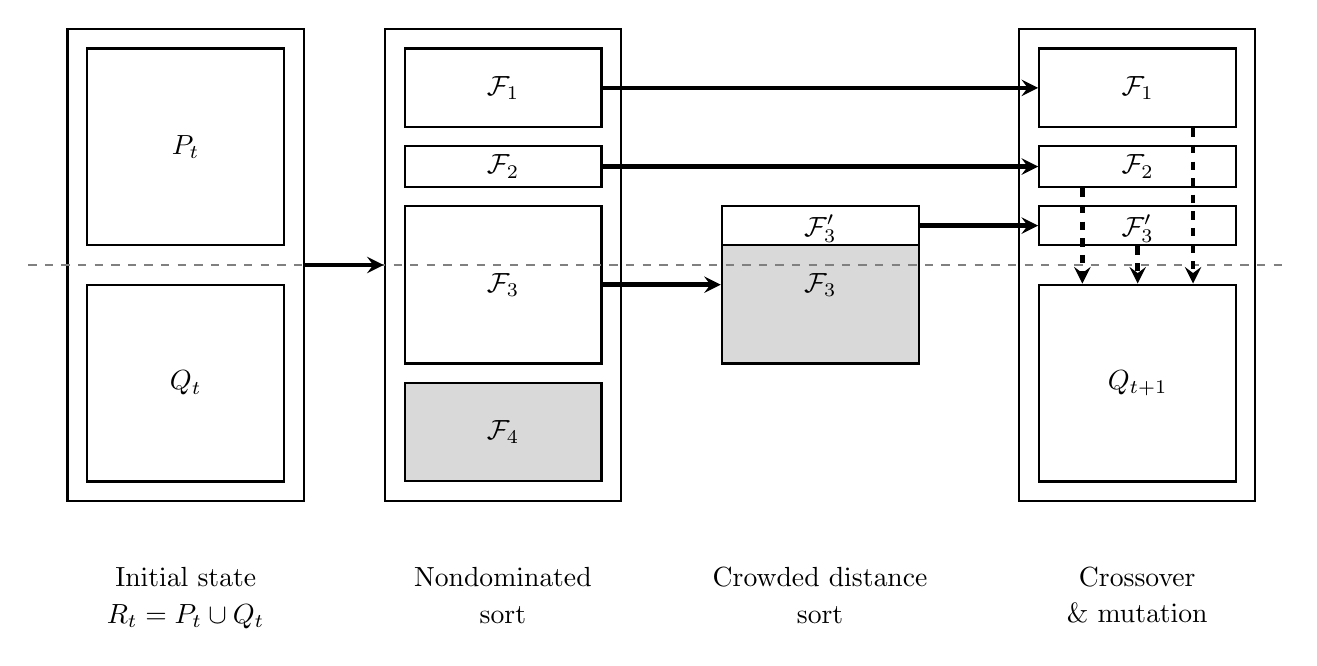
\begin{tikzpicture}
	\node (rect) at (4,2) [draw,thick,minimum width=3cm,minimum height=6cm] {};
	\node (rect1)[draw,thick,minimum width=3cm,minimum height=6cm, right = of rect] {};
	\node (rect2)[thick,minimum width=3cm,minimum height=6cm, right = of rect1] {};
	\node (rect3)[draw,thick,minimum width=3cm,minimum height=6cm, right = of rect2] {};
	\node (Pt) at (4, 3.5) [draw, thick, minimum width=2.5cm, minimum height=2.5cm] {$P_t$};
	\node (Qt) at (4, 0.5) [draw, thick, minimum width=2.5cm, minimum height=2.5cm] {$Q_t$};
	
	\node (c1) [align=center, below = 2em of rect] {Initial state\\$R_t = P_t\cup Q_t$};
	\node (c2) [align=center, below = 2em of rect1] {Nondominated\\ sort};
	\node (c3) [align=center, below = 2em of rect2] {Crowded distance\\ sort};
	\node (c4) [align=center, below = 2em of rect3] {Crossover\\ \& mutation};
	
	\node (F1) at (8.03, 4.25) [draw, thick, minimum width=2.5cm, minimum height=1cm] {$\mathcal{F}_1$};
	\node (F2) at (8.03, 3.25) [draw, thick, minimum width=2.5cm, minimum height=0.5cm] {$\mathcal{F}_2$};
	\node (F3) at (8.03, 1.75) [draw, thick, minimum width=2.5cm, minimum height=2cm] {$\mathcal{F}_3$};
	\node (F4) at (8.03, -0.12) [draw, fill=light-gray, thick, minimum width=2.5cm, minimum height=1.25cm] {$\mathcal{F}_4$};
	
	\node (F3p) at (12.06, 1.75) [draw, thick, minimum width=2.5cm, minimum height=2cm, fill=light-gray] {$\mathcal{F}_3$};
	\node (F3ap) at (12.06, 2.5) [draw, thick, minimum width=2.5cm, minimum height=0.5cm, text depth=0, fill=white] {$\mathcal{F}_3'$};
	
	\node (F1a) at (16.09, 4.25) [draw, thick, minimum width=2.5cm, minimum height=1cm] {$\mathcal{F}_1$};
	\node (F2a) at (16.09, 3.25) [draw, thick, minimum width=2.5cm, minimum height=0.5cm] {$\mathcal{F}_2$};
	\node (F3a) at (16.09, 2.5) [draw, thick, minimum width=2.5cm, minimum height=0.5cm, text depth=0] {$\mathcal{F}_3'$};
	\node (Qta) at (16.09, 0.5) [draw, thick, minimum width=2.5cm, minimum height=2.5cm] {$Q_{t+1}$};
	
	\draw[dashed, gray] (2, 2) -- (18, 2);
	
	\draw[-stealth, ultra thick] (rect) -- (rect1);
	\draw[-stealth, ultra thick] (F1) -- (F1a);
	\draw[-stealth, ultra thick] (F2) -- (F2a);
	\draw[-stealth, ultra thick] (F3) -- (F3p);
	\draw[-stealth, ultra thick] (F3ap) -- (F3a);
	
	\draw[-stealth, ultra thick, dashed] ([xshift=20pt]F1a.south) -- ([xshift=20pt]Qta.north);
	\draw[-stealth, ultra thick, dashed] ([xshift=-20pt]F2a.south) -- ([xshift=-20pt]Qta.north);
	\draw[-stealth, ultra thick, dashed] (F3a) -- (Qta);
	
\end{tikzpicture}
\caption[A single iteration of NSGA-II]{Visualisation of the stages within a single iteration of NSGA-II.}\label{fignsgaii}
\end{figure}

\subsubsection{Training algorithm}\label{sectrainmuxchn}

All the components necessary for the full implementation of a training algorithm for the multiplex chain GMHMM are now in place. From everything defined thus far, a training procedure may be easily defined as such:
\begin{enumerate}
	\item Initially, perform \emph{separate training} on all of the chains in the multiplex, using one of the individual data types involved per chain;
	\item Use NSGA-II to \emph{extract} a set of (Pareto-optimal) solutions $\boldsymbol\Omega$ for the interlayer matrix $\bomega$, that optimise the individual log-likelihoods of each training sequence;
	\item \emph{Choose} one of the extracted solutions according to a (user-defined) metric.
\end{enumerate}
I have chosen a metric that assigns larger significance to sequences with lower likelihoods, led by the idea that it is typically better to classify more sequences correctly (getting \emph{closer to the general case}) than to have superb likelihood on fewer sequences (corresponding to \emph{overfitting} the model).\\ \\
The metric I used is given by the formula
\[fit(\bomega) \myeq \sum_{i=1}^{k} i{\mathbb{L}(s_i | \bf \Theta, \boldsymbol\omega)}\]
where the $k$ training sequences have been sorted by their likelihoods in a \emph{descending} order (hence the most likely sequence gets a factor of $1$, while the least likely sequence gets a factor of $k$). The solution that is chosen as the final one is
\[\bomega^* = \argmax_{\bomega \in \boldsymbol\Omega} {fit(\bomega)}\]
The full training algorithm is summarised in Algorithm \ref{alg:muxchntrn}.
\begin{algorithm}[H]
\caption{Multiplex chain GMHMM training algorithm}\label{alg:muxchntrn}
\begin{algorithmic}[1]
\Require{Multiplex chain GMHMM $M = (n, m, L, \vec{\bf\Theta}, {\bf\bomega})$, training set $\vec{s}$ of size $k$, with $L$ data types.}
\Procedure{TrainMuxChn}{$M$, $\vec{s}$} \Comment{Train the multiplex chain GMHMM using $\vec{s}$}
	\For{$i\gets 1$ {\bf to} $L$}
		\State \Call{TrainChn}{${\bf\Theta}_i$, $\vec{s^i}$, $d$, $10^{-6}$} \Comment{Train $i$th chain using the $i$th data type}
	\EndFor	
	\For{$i\gets 1$ {\bf to} $k$} \Comment{Extracting the functions to optimise}
		\State $f_i(\bomega)\gets \mathbb{L}(s_i|{\bf\Theta},\bomega)$ \Comment{$\mathbb{L}(s_i|{\bf\Theta},\bomega)$ evaluated using the forward algorithm}
	\EndFor
	\State $\boldsymbol\Omega\gets$ \Call{NSGA-II}{$\vec{f}$, $pop$, $iter$} \Comment{Obtain Pareto-optimal solution set}
	\State $\bomega\gets\argmax\limits_{\bomega' \in \boldsymbol\Omega} {\sum\limits_{i=1}^{k} i{\mathbb{L}(s_i | \bf \Theta, \boldsymbol\omega')}}$ \Comment{Choose one of the solutions according to $fit$}
\EndProcedure
\end{algorithmic}
\end{algorithm}
\noindent A notable part of implementing this algorithm has been extracting the relevant objectives to optimise, as it utilises one of the major features introduced in \CC11---\emph{lambdas}.\\ \\
I have implemented the NSGA-II algorithm to accept an argument of type \texttt{vector<function<\textcolor{blue}{double}(vector<\textcolor{blue}{double}>)> >} for the set of functions to optimise. Within the training routine, I have filled this vector with lambda expressions that set the respective $\bomega$ values, call the forward algorithm and report its log-likelihood output (\emph{negated}, because I implemented minimisation rather than maximisation). The complete section of code is given in Listing \ref{lst:lambdae}.\\ \\
This approach is very helpful as it gives a completely \emph{generic} training procedure which does not require hard-coding the functions or having to execute the genetic algorithm separately from the main routine.
\begin{lstlisting}[caption={Code for extracting the functions to optimise, as part of the training.}, label={lst:lambdae}]
// Define the lambdas that calculate likelihoods for a given omega
objectives.resize(train_set.size());
for (uint t=0;t<train_set.size();t++)
{
	objectives[t] = [this, t, &train_set] (vector<double> X) -> double
	{
		double **temp_omega = new double*[L];
		for (int i=0;i<L;i++)
		{
			temp_omega[i] = new double[L];
			for (int j=0;j<L;j++)
			{
				temp_omega[i][j] = X[i*L + j];
			}
		}
            
		set_omega(temp_omega);
            
		for (int i=0;i<L;i++) delete[] temp_omega[i];
		delete[] temp_omega;
            
		return -log_likelihood(train_set[t]);
	};
}
\end{lstlisting}

\section{Full multiplex GMHMM}\label{secfullgmhmm}

After fully implementing the core deliverable, a fitting next step is to \emph{extend it} to take advantage of the full power and flexibility of the unconstrained GMHMM. As the models are highly similar, this section will focus on outlining the main implementation differences between them, and then discussing the major differences in detail.

\subsection{Implementation differences}

In this subsection, I will present the differences between the multiplex chain GMHMM and the full multiplex GMHMM in the form of bullet points, for clarity.

\subsubsection{State} 

\begin{itemize}
	\item There are still $L$ GMHMM layers involved, each one trained on a unique data type from the training sequences.
	\item The structure of each layer is no longer constrained to be a chain; an arbitrary configuration using $n$ states is allowed. As such, the state transition matrix, $\bf T$, must be specified.
	\item As it is no longer required for the GMHMM to always follow a specific path, the interlayer edges may now point from a node to itself; the edges themselves are still stored in the form of a matrix, $\bomega$. This means that the transition probabilities within the $i$th layer, ${\bf T}_i$, will effectively be scaled by $\bomega_{ii}$.
\end{itemize}

\subsubsection{Algorithms}
\begin{itemize}
	\item Likelihoods are calculated as before; using the forward algorithm (\cref{secfwdalgs}).
	\item Parameter estimation of $\vec{\mu}$ and $\vec{\sigma}$ is still performed using the method described in \cref{secparest}. However, as the states no longer need to have any fixed meaning, the sub-output emission probabilities $\bf O'$ are no longer trained in this way.
	\item The parameters $\vec{\pi}$, $\bf T$ and $\bf O'$ are to be trained using a generic unsupervised learning algorithm for HMMs; in my project I have employed the most commonly used \underline{\emph{Baum-Welch}} algorithm for this purpose.
	\item Training of the interlayer transition matrix $\bomega$ is performed using the same call to NSGA-II as described in \cref{sectrainmuxchn}.
\end{itemize}

\subsection{Baum-Welch algorithm}\label{secbaumwelch}

Most of the differences given above are minor and represent simple extensions; the only major difference is contained within the training procedure for a single layer GMHMM; the {\bf Baum-Welch algorithm} \cite{rabiner1989tutorial}. Its aim is to produce, from a given HMM $\bf\Theta$ and output sequence $(\vec{y}, \vec{id})$, a new HMM $\bf\Theta'$ that is more likely to produce $(\vec{y}, \vec{id})$; i.e.
\[\mathbb{L}(\vec{y}, \vec{id}|{\bf \Theta'}) \geq \mathbb{L}(\vec{y}, \vec{id}|{\bf \Theta})\]
This procedure could then be iterated a set number of times, until the desirable level of convergence is achieved.

\subsubsection{EM iteration}\label{secemiter}

The Baum-Welch algorithm is an HMM-specific implementation of the more generalised \emph{Expectation-Maximisation (EM)} algorithm \cite{dempster1977maximum}. A single iteration operates as follows:
\begin{enumerate}
	\item \emph{(E step)} Evaluate the probabilities of being in state $x$ at time $t$, $\gamma_x(t)$:
	\[\gamma_x(t) \myeq \mathbb{P}(X_t = x | \vec{y}, \vec{id}, {\bf\Theta})\]
	and the probabilities of transitioning from state $i$ to state $j$ at time $t$, $\xi_{ij}(t)$:
	\[\xi_{ij}(t) \myeq \mathbb{P}(X_t = i, X_{t+1} = j | \vec{y}, \vec{id}, {\bf\Theta})\]
	\item \emph{(M step)} Update the parameters of ${\bf\Theta}$ as follows:
	\begin{enumerate}
		\item The start-state probabilities, $\pi'_x$, simply correspond to the probabilities of being in state $x$ at time $1$:
				\[\pi'_x = \gamma_x(1)\]
		\item The transition probabilities, ${\bf T}'_{ij}$, may be calculated as the probabilities that the model will move to state $j$, after previously being located in state $i$:
				\[{\bf T}'_{ij} = \frac{\sum\limits_{t=1}^{T-1}{\xi_{ij}(t)}}{\sum\limits_{t=1}^{T-1}{\gamma_i(t)}}\]
		\item The sub-output emission probabilities, ${\bf O''}_{xy'}$, are evaluated as the probabilities that sub-output $y'$ will be produced, given that the model is in state $x$:
			\[{\bf O''}_{xy'} = \frac{\sum\limits_{t=1}^{T}{\mathbb{I}(id_t = y')}\gamma_x(t)}{\sum\limits_{t=1}^{T}{\gamma_x(t)}}\]
			where $\mathbb{I}$ is the indicator function ($1$ if $id_t = y$, $0$ otherwise).
	\end{enumerate}
		obtaining the new model ${\bf\Theta'} = (\vec{\pi}', {\bf T'}, {\bf O''})$.
\end{enumerate}
In order to properly perform the \emph{E step}, additional information is needed.\\ \\ The forward algorithm provides us with $\alpha_t(x)$, the likelihoods of ending up in state $x$ at time $t$ and producing the first $t$ elements of the output sequence. However, for $\gamma_x(t)$ it is needed to evaluate this probability conditional on the \emph{entire} output sequence. Clearly, an algorithm is needed to evaluate the likelihoods of producing the corresponding \emph{suffices} of the output sequence, assuming we start in state $x$. This algorithm will be described in the next paragraph.

\subsubsection{Backward algorithm}

The quantities referred to at the end of the previous part, the \textbf{backward likelihoods} $\beta_t(x)$, are the likelihoods of observing the output sequence from time $t+1$ onwards, assuming we are in state $x$ at time $t$, i.e.
\[\beta_t(x) \myeq \mathbb{L}(\{(y_i, id_i)\}_{i={t+1}}^{T} | x_t = x, {\bf\Theta})\]
The backward likelihoods may efficiently be computed by the \textbf{backward algorithm}, which could be imagined as a \emph{``reversed''} version of the forward algorithm.\\ \\
The \emph{base cases} are this time $\beta_T(x) = 1$, as the probability of observing an empty sequence is 1, regardless of which state we start from. The recurrence relation used to calculate $\beta_t(x)$, given that $\beta_{t+1}(x)$ had already been calculated for all $x$, may be derived (in a similar way as was done for $\alpha_t(x)$) to be:
\[\begin{aligned}
\beta_{t}(x) & = \mathbb{L}(\{(y_i, id_i)\}_{i=t+1}^{T} | x_{t} = x, {\bf \Theta})\\
& = \sum_{x'\in S}{\mathbb{L}(\{(y_i, id_i)\}_{i=t+1}^{T}, x_{t+1} = x' | x_{t} = x, {\bf \Theta})}\\
& = \sum_{x'\in S}{\mathbb{L}(x_{t+1} = x'| x_{t} = x, {\bf \Theta})\mathbb{L}(\{(y_i, id_i)\}_{i=t+1}^{T} | x_{t+1} = x', x_{t} = x, {\bf \Theta})}\\
& = \sum_{x'\in S}{{\bf T}_{xx'}\mathbb{L}(\{(y_i, id_i)\}_{i=t+1}^{T} | x_{t+1} = x', {\bf \Theta})}\\
& = \sum_{x'\in S}{{\bf T}_{xx'}\mathbb{L}((y_{t+1}, id_{t+1}) | x_{t+1} = x', {\bf \Theta})\mathbb{L}(\{(y_i, id_i)\}_{i=t+2}^{T} | x_{t+1} = x', {\bf \Theta})}\\
& = \sum_{x'\in S}{{\bf T}_{xx'}{\bf O'}_{x',id_{t+1}}\mathcal{N}(y_{t+1}; \mu_{id_{t+1}}, \sigma_{id_{t+1}})\beta_{t+1}(x')}\\
\end{aligned}\]
Similar underflow-avoiding techniques could be utilised for the backward algorithm as for the forward algorithm; namely, it is common to re-use the scaling coefficients $\vec{c}$ used to scale $\alpha_t(x)$, and let the actually stored value be 
\[\hat{\beta}_t(x) = c_{t+1}\beta_t(x)\] 
(specially, $\beta_T(x)$ is not scaled). Note that scaling by $c_{t+1}$ does not need to normalise the values of $\beta_t(x)$, however it does simplify the E step performed afterwards.\\ \\
The pseudocode of the entire procedure is highly similar to the forward algorithm (given in Algorithm \ref{alg:fwd}), and as such is omitted from this paragraph; the time complexity of the backward algorithm is $O(n^2\cdot T)$, same as for the forward algorithm.

\subsubsection{E step}

Now that the backward likelihoods have been evaluated, it is possible to combine them with the forward likelihoods to obtain the quantities $\gamma_x(t)$ and $\xi_{ij}(t)$. The probability $\gamma_x(t)$ may be evaluated as the \emph{normalised likelihood} of being in state $x$ at time $t$:
\[
\gamma_x(t) = \mathbb{P}(X_t = x | \vec{y}, \vec{id}, {\bf\Theta}) = \frac{\mathbb{L}(X_t = x | \vec{y}, \vec{id}, {\bf\Theta})}{\sum\limits_{x'\in s}{\mathbb{L}(X_t = x' | \vec{y}, \vec{id}, {\bf\Theta})}}
\]
$\mathbb{L}(X_t = x | \vec{y}, \vec{id}, {\bf\Theta})$ may be evaluated using Bayes' theorem:
\[\begin{aligned}
\mathbb{L}(X_t = x | \vec{y}, \vec{id}, {\bf\Theta}) &= \frac{\mathbb{L}(\vec{y}, \vec{id} | X_t = x, {\bf\Theta})\mathbb{L}(X_t = x|{\bf\Theta})}{\mathbb{L}(\vec{y}, \vec{id}|{\bf\Theta})}\\
&= \frac{\mathbb{L}(\{(y_i, id_i)\}_{i=1}^{t} | X_t = x, {\bf\Theta})\mathbb{L}(X_t = x|{\bf\Theta})\mathbb{L}(\{(y_i, id_i)\}_{i=t+1}^{T} | X_t = x, {\bf\Theta})}{\mathbb{L}(\vec{y}, \vec{id}|{\bf\Theta})}\\
&= \frac{\mathbb{L}(\{(y_i, id_i)\}_{i=1}^{t}, X_t = x | {\bf\Theta})\mathbb{L}(\{(y_i, id_i)\}_{i=t+1}^{T} | X_t = x, {\bf\Theta})}{\mathbb{L}(\vec{y}, \vec{id}|{\bf\Theta})}\\
&= \frac{\alpha_t(x)\beta_t(x)}{\mathbb{L}(\vec{y}, \vec{id}|{\bf\Theta})}\\
\end{aligned}\]
Expressing $\mathbb{L}(\vec{y}, \vec{id}|{\bf\Theta})$ using the scaling coefficients $\vec{c}$:
\[\begin{aligned}
\mathbb{L}(X_t = x | \vec{y}, \vec{id}, {\bf\Theta}) &= \frac{\alpha_t(x)\beta_t(x)}{\mathbb{L}(\vec{y}, \vec{id}|{\bf\Theta})}\\
&= \frac{\alpha_t(x)\beta_t(x)}{\prod\limits_{s=1}^{T}{c_s^{-1}}}\\
&= \left(\alpha_t(x)\prod_{s=1}^{t}{c_s}\right)\left(\beta_t(x)\prod_{s=t+1}^{T}{c_s}\right) = \hat{\alpha}_t(x)\hat{\beta}_t(x)
\end{aligned}\]
Therefore, $\gamma_x(t)$ may be simply calculated as
\[\gamma_x(t)=\frac{\hat{\alpha}_t(x)\hat{\beta}_t(x)}{\sum\limits_{x'\in S}{\hat{\alpha}_t(x')\hat{\beta}_t(x')}}\]
Similarly, the probability $\xi_{ij}(t)$ may be interpreted as the normalised likelihood of taking the transition $i\longrightarrow j$ at time $t$:
\[\xi_{ij}(t) = \mathbb{P}(X_t = i, X_{t+1} = j | \vec{y}, \vec{id}, {\bf\Theta}) = \frac{\mathbb{L}(X_t = i, X_{t+1} = j | \vec{y}, \vec{id}, {\bf\Theta})}{\sum\limits_{a\in S}\sum\limits_{b\in S}\mathbb{L}(X_t = a, X_{t+1} = b | \vec{y}, \vec{id}, {\bf\Theta})}\]
Using the model assumptions and Bayes' theorem, $\mathbb{L}(X_t = i, X_{t+1} = j | \vec{y}, \vec{id}, {\bf\Theta})$ may also be defined in terms of the parameters we already know (steps omitted---refer to Figure \ref{figxii} for an illustration of the formula):
\[\begin{aligned}\mathbb{L}(X_t = i, X_{t+1} = j | \vec{y}, \vec{id}, {\bf\Theta}) &= \frac{\alpha_t(i){\bf T}_{ij}{\bf O'}_{j,id_{t+1}}\mathcal{N}(y_{t+1}; \mu_{id_{t+1}}, \sigma_{id_{t+1}})\beta_{t+1}(j)}{\prod\limits_{s=1}^T{c_s^{-1}}}\\
&= c_{t+1}\hat{\alpha}_t(i){\bf T}_{ij}{\bf O'}_{j,id_{t+1}}\mathcal{N}(y_{t+1}; \mu_{id_{t+1}}, \sigma_{id_{t+1}})\hat{\beta}_{t+1}(j)\\
\end{aligned}\]

\begin{figure}[H]
\begin{center}
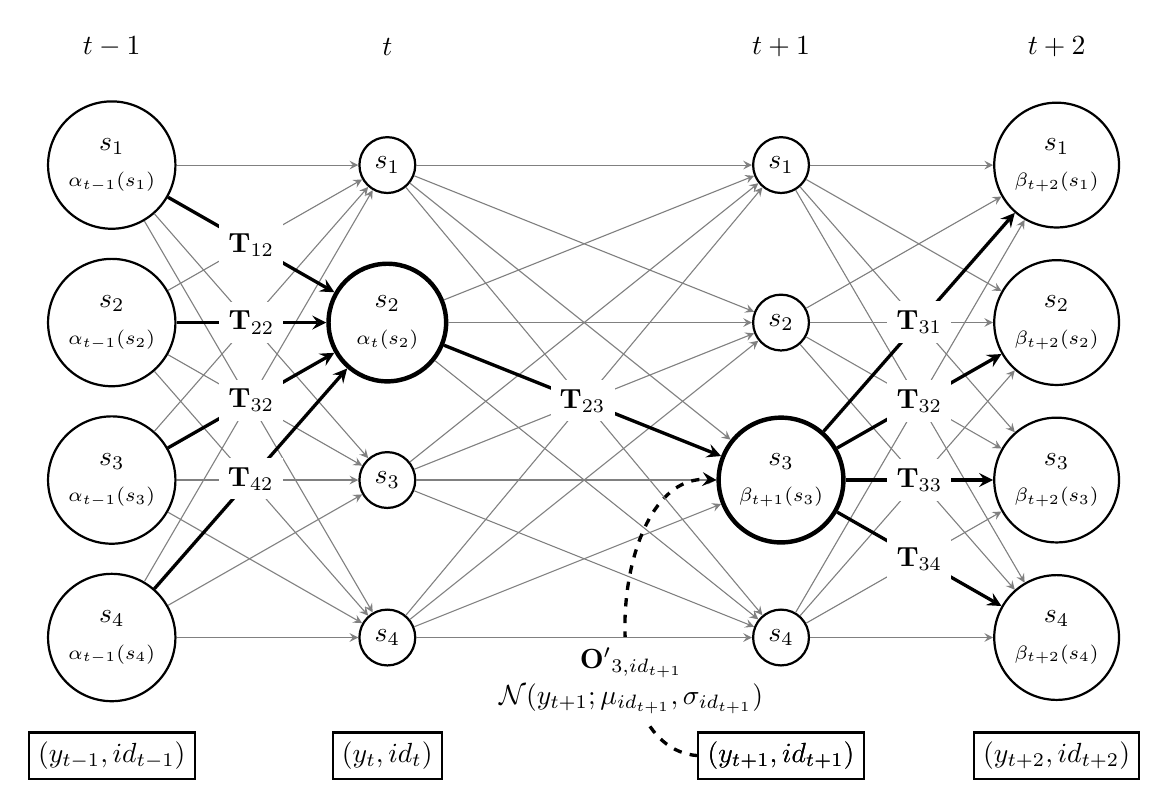
\begin{tikzpicture}[]
% 1st column
\node               at (0,6.5) {$t-1$};
\node[align=center, circle, draw, thick] (s1_1) at (0,5) {$s_1$\\{\scriptsize$\alpha_{t-1}(s_1)$}};
\node[align=center, circle, draw, thick] (s2_1) at (0,3) {$s_2$\\{\scriptsize$\alpha_{t-1}(s_2)$}};
\node[align=center, circle, draw, thick] (s3_1) at (0,1) {$s_3$\\{\scriptsize$\alpha_{t-1}(s_3)$}};
\node[align=center, circle, draw, thick] (s4_1) at (0,-1) {$s_4$\\{\scriptsize$\alpha_{t-1}(s_4)$}};
\node [draw, thick] at (0,-2.5) {$(y_{t-1}, id_{t-1})$};
% 2nd column
\node               at (3.5,6.5) {$t$};
\node[circle, draw, thick] (s1_2) at (3.5,5) {$s_1$}
    edge[gray, thin, stealth-] (s1_1)
    edge[gray, thin, stealth-] (s2_1)
    edge[gray, thin, stealth-] (s3_1)
    edge[gray, thin, stealth-] (s4_1);
\node[circle, draw, thick] (s3_2) at (3.5,1) {$s_3$}
    edge[gray, thin, stealth-] (s1_1)
    edge[gray, thin, stealth-] (s2_1)
    edge[gray, thin, stealth-] (s3_1)
    edge[gray, thin, stealth-] (s4_1);
\node[circle, draw, thick] (s4_2) at (3.5,-1) {$s_4$}
    edge[gray, thin, stealth-] (s1_1)
    edge[gray, thin, stealth-] (s2_1)
    edge[gray, thin, stealth-] (s3_1)
    edge[gray, thin, stealth-] (s4_1);
\node[align=center, circle, draw, ultra thick, minimum size=4.25em] (s2_2) at (3.5,3) {$s_2$\\{\scriptsize$\alpha_{t}(s_2)$}};
%3rd column
\node [] (asdf2) at (8.5,-2.5) {$(y_{t+1}, id_{t+1})$};
\node [draw, thick] (asdf3) at (12,-2.5) {$(y_{t+2}, id_{t+2})$};
\node[align=center, circle, draw, ultra thick, minimum size=4.25em] (s3_3) at (8.5,1) {$s_3$\\{\scriptsize$\beta_{t+1}(s_3)$}}
    edge[gray, thin, stealth-] (s1_2)
    edge[gray, thin, stealth-] (s3_2)
    edge[gray, thin, stealth-] (s4_2);
\draw[-stealth, very thick, dashed, bend left=90] (asdf2.west) to node[pos=0.33, align=center, fill=white] {${\bf O'}_{3,id_{t+1}}$\\$\mathcal{N}(y_{t+1};\mu_{id_{t+1}},\sigma_{id_{t+1}})$} (s3_3.west);
\node [draw, thick] (asdf2) at (8.5,-2.5) {$(y_{t+1}, id_{t+1})$};
\node               at (8.5,6.5) {$t+1$};
\node[circle, draw, thick] (s1_3) at (8.5,5) {$s_1$}
    edge[gray, thin, stealth-] (s1_2)
    edge[gray, thin, stealth-] (s2_2)
    edge[gray, thin, stealth-] (s3_2)
    edge[gray, thin, stealth-] (s4_2);
\node[circle, draw, thick] (s2_3) at (8.5,3) {$s_2$}
    edge[gray, thin, stealth-] (s1_2)
    edge[gray, thin, stealth-] (s2_2)
    edge[gray, thin, stealth-] (s3_2)
    edge[gray, thin, stealth-] (s4_2);
\node[circle, draw, thick] (s4_3) at (8.5,-1) {$s_4$}
    edge[gray, thin, stealth-] (s1_2)
    edge[gray, thin, stealth-] (s2_2)
    edge[gray, thin, stealth-] (s3_2)
    edge[gray, thin, stealth-] (s4_2);
%4th column
\node               at (12,6.5) {$t+2$};
\node[align=center, circle, draw, thick] (s1_4) at (12,5) {$s_1$\\{\scriptsize$\beta_{t+2}(s_1)$}}
    edge[gray, thin, stealth-] (s1_3)
    edge[gray, thin, stealth-] (s2_3)
    edge[gray, thin, stealth-] (s4_3);
\node[align=center, circle, draw, thick] (s2_4) at (12,3) {$s_2$\\{\scriptsize$\beta_{t+2}(s_2)$}}
    edge[gray, thin, stealth-] (s1_3)
    edge[gray, thin, stealth-] (s2_3)
    edge[gray, thin, stealth-] (s4_3);
\node[align=center, circle, draw, thick] (s3_4) at (12,1) {$s_3$\\{\scriptsize$\beta_{t+2}(s_3)$}}
    edge[gray, thin, stealth-] (s1_3)
    edge[gray, thin, stealth-] (s2_3)
    edge[gray, thin, stealth-] (s4_3);
\node[align=center, circle, draw, thick] (s4_4) at (12,-1) {$s_4$\\{\scriptsize$\beta_{t+2}(s_4)$}}
    edge[gray, thin, stealth-] (s1_3)
    edge[gray, thin, stealth-] (s2_3)
    edge[gray, thin, stealth-] (s4_3);
\draw[very thick, stealth-]
    (s2_2) to node [midway, fill=white] {${\bf T}_{12}$} (s1_1);
\draw[very thick, stealth-]
    (s2_2) to node [midway, fill=white] {${\bf T}_{22}$} (s2_1);
\draw[very thick, stealth-]
    (s2_2) to node [midway, fill=white] {${\bf T}_{32}$} (s3_1);
\draw[very thick, stealth-]
    (s2_2) to node [midway, fill=white] {${\bf T}_{42}$} (s4_1);
\draw[very thick, stealth-]
    (s1_4) to node [midway, fill=white] {${\bf T}_{31}$} (s3_3);
\draw[very thick, stealth-]
    (s2_4) to node [midway, fill=white] {${\bf T}_{32}$} (s3_3);
\draw[very thick, stealth-]
    (s3_4) to node [midway, fill=white] {${\bf T}_{33}$} (s3_3);
\draw[very thick, stealth-]
    (s4_4) to node [midway, fill=white] {${\bf T}_{34}$} (s3_3);
\draw[very thick, stealth-]
    (s3_3) to node [midway, fill=white] {${\bf T}_{23}$} (s2_2);
\node [draw, thick] (asdf) at (3.5,-2.5) {$(y_{t}, id_{t})$};
\end{tikzpicture}
\end{center}
\caption[Illustration of the transition probability formula]{\centering Illustration of the formula used to calculate $\Like(X_t=i,X_{t+1}=j|\vec{y},\vec{id},{\bf\Theta})$, on a four-state GMHMM, with $i=s_2$ and $j=s_3$.}\label{figxii}
\end{figure}
\noindent Therefore, $\xi_{ij}(t)$ may be calculated as
\[\begin{aligned}
\xi_{ij}(t) &= \frac{c_{t+1}\hat{\alpha}_t(i){\bf T}_{ij}{\bf O'}_{j,id_{t+1}}\mathcal{N}(y_{t+1}; \mu_{id_{t+1}}, \sigma_{id_{t+1}})\hat{\beta}_{t+1}(j)}{\sum\limits_{a\in S}\sum\limits_{b\in S}c_{t+1}\hat{\alpha}_t(a){\bf T}_{ab}{\bf O'}_{b,id_{t+1}}\mathcal{N}(y_{t+1}; \mu_{id_{t+1}}, \sigma_{id_{t+1}})\hat{\beta}_{t+1}(b)}\\
&= \frac{c_{t+1}\hat{\alpha}_t(i){\bf T}_{ij}{\bf O'}_{j,id_{t+1}}\mathcal{N}(y_{t+1}; \mu_{id_{t+1}}, \sigma_{id_{t+1}})\hat{\beta}_{t+1}(j)}{\sum\limits_{a\in S}\hat{\alpha}_t(a)c_{t+1}\sum\limits_{b\in S}{\bf T}_{ab}{\bf O'}_{b,id_{t+1}}\mathcal{N}(y_{t+1}; \mu_{id_{t+1}}, \sigma_{id_{t+1}})\hat{\beta}_{t+1}(b)}\\
&= \frac{c_{t+1}\hat{\alpha}_t(i){\bf T}_{ij}{\bf O'}_{j,id_{t+1}}\mathcal{N}(y_{t+1}; \mu_{id_{t+1}}, \sigma_{id_{t+1}})\hat{\beta}_{t+1}(j)}{\sum\limits_{a\in S}\hat{\alpha}_t(a)\hat{\beta}_{t}(a)}
\end{aligned}\]
This concludes the E step of the algorithm.

\subsubsection{Full algorithm}

With a method of computing $\gamma_x(t)$ and $\xi_{ij}(t)$ in place, the M step is trivially performed by just evaluating the formulae given in \cref{secemiter}. With this in mind, the pseudocode of the Baum-Welch algorithm is given in Algorithm \ref{alg:baumwelch}.\\ \\
The time complexity of the forward-backward step is $O(n^2\cdot T)$, as previously discussed; the E step requires $O(n^2\cdot T)$ time, and the M step requires $O((n^2 + n\cdot m)\cdot T)$ time. Therefore, the time complexity of a single Baum-Welch iteration is dominated by the M step, i.e. $O((n^2 + n\cdot m)\cdot T)$. Storing the function $\xi_{ij}(t)$ would require a space complexity of $O(n^2\cdot T)$, however, storing this parameter is not necessary (as it may be computed ad-hoc during the M step); hence the iteration's overall space complexity equals that of the forward/backward algorithms.
\begin{algorithm}[H]
\caption{Baum-Welch algorithm}\label{alg:baumwelch}
\begin{algorithmic}[1]
\Require{GMHMM ${\bf\Theta} = (n, m, \vec{\pi}, {\bf T}, {\bf O'}, \vec{\mu}, \vec{\sigma})$, output sequence $(\vec{y}, \vec{id})$ of length $T$.}
\Procedure{BaumWelch}{$\bf\Theta$, $\vec{y}$, $\vec{id}$, $T$} \Comment{Generate a more fit model wrt ($\vec{y}$, $\vec{id}$)}
	\State $(\hat{\alpha}, \vec{c}, \ell)\gets$ \Call{Forward}{$\bf\Theta$, $\vec{y}$, $\vec{id}$, $T$} \Comment{Run the forward algorithm}
	\State $\hat{\beta}\gets$ \Call{Backward}{$\bf\Theta$, $\vec{y}$, $\vec{id}$, $T$, $\vec{c}$} \Comment{Run the backward algorithm, reusing $\vec{c}$}
	\For{$t\gets 1$ {\bf to} $T$} \Comment{E step; calculating $\gamma_x(t)$ and $\xi_{ij}(t)$}
		\For{$i\gets 1$ {\bf to} $n$}
			\State $s\gets \sum\limits_{x\in S}{\hat{\alpha}_t(x)\hat{\beta}_t(x)}$
			\State $\gamma_i(t)\gets\frac{\hat{\alpha}_t(i)\hat{\beta}_t(i)}{s}$
			\For{$j\gets 1$ {\bf to} $n$}
				\State $\xi_{ij}(t)\gets \frac{c_{t+1}\hat{\alpha}_t(i){\bf T}_{ij}{\bf O'}_{j,id_{t+1}}\mathcal{N}(y_{t+1}; \mu_{id_{t+1}}, \sigma_{id_{t+1}})\hat{\beta}_{t+1}(j)}{s}$
			\EndFor
		\EndFor
	\EndFor
	\For{$i\gets 1$ {\bf to} $n$} \Comment{M step; reestimating $\vec{\pi}$, $\bf T$ and $\bf O'$}
		\State $\pi_i\gets \gamma_1(i)$
		\For{$j\gets 1$ {\bf to} $n$}
			\State ${\bf T}_{ij}\gets\frac{\sum\limits_{t=1}^{T-1}{\xi_{ij}(t)}}{\sum\limits_{t=1}^{T-1}{\gamma_i(t)}}$
		\EndFor
		\For{$y'\gets 1$ {\bf to} $m$}
			\State ${\bf O'}_{iy'}\gets\frac{\sum\limits_{t=1}^{T}{\mathbb{I}(id_t=y')\gamma_i(t)}}{\sum\limits_{t=1}^T{\gamma_i(t)}}$
		\EndFor
	\EndFor
\EndProcedure
\end{algorithmic}
\end{algorithm}

\subsubsection{Multiple sequence training}
Thus far, I have discussed an implementation of the Baum-Welch algorithm that takes only a \textbf{single} sequence for training. However, as previously discussed, within the context of my project it is more likely that \emph{multiple shorter sequences} will be used. I will hence conclude the discussion of the Baum-Welch algorithm with an overview of extending it for training on $k$ separate sequences \cite{rabiner1989tutorial}.\\ \\
Luckily, as the re-estimation formulae for ${\bf T}_{ij}$ and ${\bf O'}_{iy'}$ simply measure the frequencies of their respective transitions and emissions, it suffices to run the forward-backward procedure and E step on each of the sequences (producing $\gamma_x^\ell(t)$ and $\xi_{ij}^\ell(t)$ for the $\ell$-th sequence), and then simply summing up contributions from every sequence:
\[{\bf T}'_{ij} = \frac{\sum\limits_{\ell=1}^k\sum\limits_{t=1}^{T-1}{\xi_{ij}^\ell(t)}}{\sum\limits_{\ell=1}^k\sum\limits_{t=1}^{T-1}{\gamma_i^\ell(t)}}\]
\[{\bf O''}_{xy'} = \frac{\sum\limits_{\ell=1}^k\sum\limits_{t=1}^{T}{\mathbb{I}(id_t^\ell = y')}\gamma_x^\ell(t)}{\sum\limits_{\ell=1}^k\sum\limits_{t=1}^{T}{\gamma_x^\ell(t)}}\]
The formula for re-estimating $\pi_x$ may also be trivially modified, by considering an equiprobable sum of each of the sequences' initial state distributions:
\[\pi'_x = \frac{1}{k}\sum_{\ell=1}^k{\gamma_x^\ell(1)}\]
It should be clear that very few changes are needed to Algorithm \ref{alg:baumwelch} in order to make a \textsc{BaumWelch} procedure capable of handling multiple sequences; as such, the full pseudocode is omitted from this paragraph.

\subsection{Training}\label{secfulltrn}

Having implemented the Baum-Welch algorithm, I had all the necessary pieces to finalise the training algorithm; it is summarised in Algorithm \ref{alg:fullmuxtrn}.
\begin{algorithm}[H]
\caption{Full multiplex GMHMM training algorithm}\label{alg:fullmuxtrn}
\begin{algorithmic}[1]
\Require{Full multiplex GMHMM $M = (n, m, L, \vec{\bf\Theta}, {\bf\bomega})$, training set $\vec{s}$ of size $k$, and lengths $\vec{T}$ with $L$ data types.}
\Procedure{TrainMuxGMHMM}{$M$, $\vec{s}$, $\vec{T}$} \Comment{Train the multiplex GMHMM using $\vec{s}$}
	\For{$i\gets 1$ {\bf to} $L$}
		\State \Call{TrainGauss}{${\bf\Theta}_i$, $\vec{s^i}$} \Comment{Estimate the parameters $\vec{\mu}_i$ and $\vec{\sigma}_i$}
		\State \Call{BaumWelch}{${\bf\Theta}_i$, $\vec{s^i}$, $\vec{T^i}$} \Comment{Train $i$th GMHMM using the $i$th data type}
	\EndFor	
	\For{$i\gets 1$ {\bf to} $k$} \Comment{Extracting the functions to optimise}
		\State $f_i(\bomega)\gets \mathbb{L}(s_i|{\bf\Theta},\bomega)$ \Comment{$\mathbb{L}(s_i|{\bf\Theta},\bomega)$ evaluated using the forward algorithm}
	\EndFor
	\State $\boldsymbol\Omega\gets$ \Call{NSGA-II}{$\vec{f}$, $pop$, $iter$} \Comment{Obtain Pareto-optimal solution set}
	\State $\bomega\gets\argmax\limits_{\bomega' \in \boldsymbol\Omega} {\sum\limits_{i=1}^{k} i{\mathbb{L}(s_i | \bf \Theta, \boldsymbol\omega')}}$ \Comment{Choose one of the solutions according to $fit$}
\EndProcedure
\end{algorithmic}
\end{algorithm}
\noindent Note that the algorithm as presented shares many similarities with the chain GMHMM training algorithm (\cref{sectrainmuxchn}); the only difference is the way the individual layers are trained. With this I conclude the discussion of the full multiplex GMHMM, and with it, the entire implementation phase of the project.

%\section{Aggregate multiplex model}\label{secaggr}

%\subsection{Communicability}

%\subsection{Matrix exponential}

\section{Summary}

This chapter has summarised the entire implementation phase that resulted in successfully achieving the core and extension machine learning model deliverables; in particular, I have given a detailed discussion of the key algorithms used for evaluating output likelihoods and model training, and demonstrated how those building blocks may be combined into a model used for binary classification.\\ \\
The next chapter will focus on the evaluation phase of the project, reviewing the methods used to ascertain the correct behaviour of the models, as well as examining the extent to which the implemented models have accomplished their success criteria.

\chapter{Evaluation}

\emph{Having thoroughly reviewed the implementation of my project, in this chapter I will aim to demonstrate evidence that the project has successfully achieved all of the success criteria outlined in its original proposal.\\ \\
This will include an overview of the methods I have used to verify that the implemented models behave as proposed, followed by a comparative evaluation using synthetic and biomolecular data (where I will demonstrate that introducing multiplexity produces a  significant rise in classifier performance, as predicted), and assessment of the robustness of the models in presence of experimental error.}

\section{Success criteria}

The evaluation of my project first required thinking back to the project's main success criteria outlined in its proposal (Appendix \ref{secprop}), in order to be able to assess whether they have been achieved. They are summarised in this section, along with pointers to the areas of the dissertation where their successful achievement is demonstrated. I have denoted a successfully met criterion with a tick (\checkmark), adding an additional tick if the criterion had been extended in some way.
\begin{enumerate}[label=\bf Criterion \arabic*:]
	\item \emph{The complete proposed classifier data structure should be implemented, incorporating at least the three main building blocks\dots [Chain GMHMM, Multiplex, NSGA-II].}\\
		This refers to the successful core project implementation, which has been thoroughly demonstrated in \cref{secmuxchngmhmm}. \checkmark\ Furthermore, a completely generalised multiplex GMHMM was successfully implemented, as described in \cref{secfullgmhmm}. \checkmark
	\item \emph{Correct operation of the individual modules within the structure should be tested on the sample tests provided in relevant literature or academic papers.}\\
		I have met this criterion by implementing a variety of \emph{unit tests} on the key algorithms used in the models; these will be outlined in \cref{secunittests} and have been setup for both the core and extension components. \checkmark\checkmark
	\item \emph{The accuracy of the classifier should be evaluated with at least the two methods \dots (supervised learning setup to estimate accuracy, and comparison with single-layered classifiers). It might prove useful to provide further ways of evaluation\dots}\\
		This refers to successfully implementing an evaluation suite as prescribed by the criterion; I was successful in this as well, and the results of the comparative evaluation are given in \cref{seccompeval}. \checkmark\ Furthermore, I have extended the suite with \emph{noise testing}, in order to investigate the robustness of the models in the presence of experimental errors; the results of this analysis are summarised in \cref{secnojz}. \checkmark
\end{enumerate}

\section{Unit tests}\label{secunittests}

As prescribed by Criterion 2, I have utilised a variety of known examples from relevant academic papers, presentations or literature in order to properly verify that the principal algorithms are operating as expected. The key algorithms covered by unit testing, along with their respective source used for the test, are given in Table \ref{tbldut}. The exact tests (with expected outputs) are presented in Appendix \ref{secapptests}.
\begin{table}[H]\centering
\begin{tabular}{ l  r } \toprule
{\bf Algorithm under test} & {\bf Test source}\\ \midrule
Forward/backward algorithm & Russell \& Norvig \cite{Russell:2003:AIM:773294}\\
Baum-Welch algorithm & Frazzoli \cite{FrazzoliMIT}\\
NSGA-II & Deb \emph{et al.} \cite{deb2002fast}\\
\bottomrule
\end{tabular}
\caption[A summary of the unit tests on key algorithms]{A summary of the unit tests on key algorithms within the project.}\label{tbldut}
\end{table} 
\noindent The unit tests have been implemented either as standalone \CC\ programs or shell scripts; a screenshot of recompiling and executing one of them is given in Figure \ref{figunit}.
\begin{figure}[h]
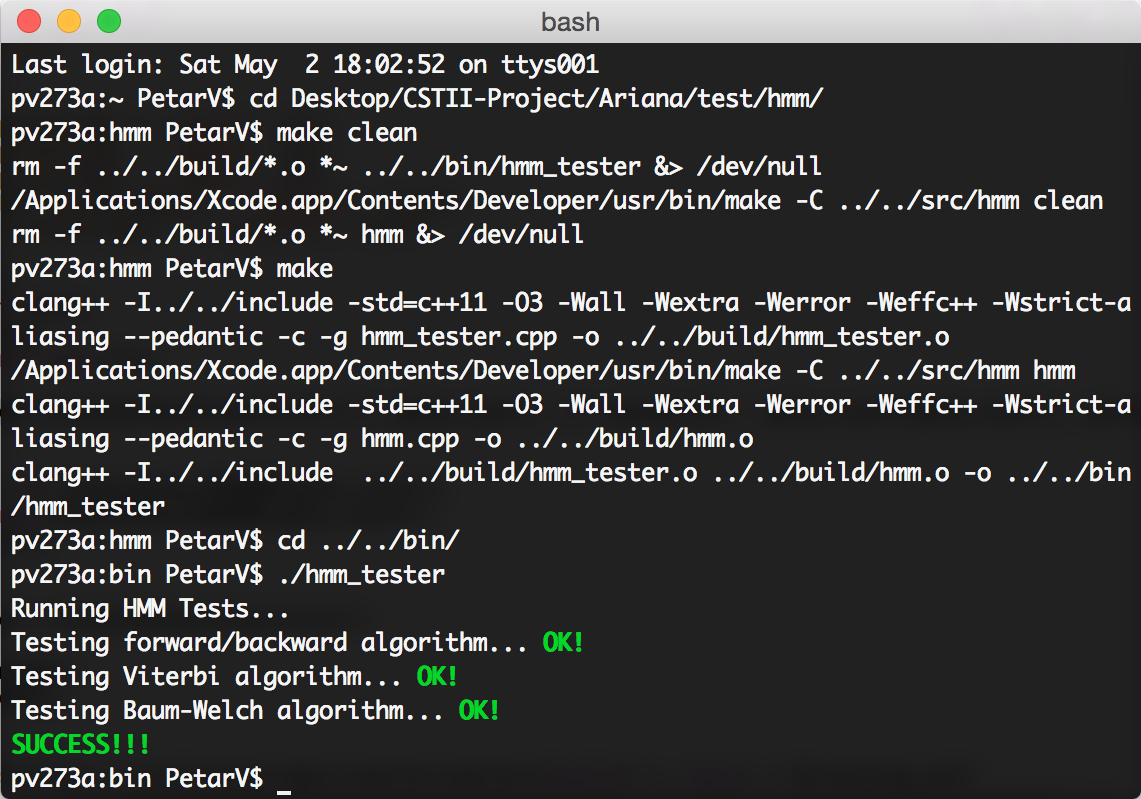
\includegraphics[width=\linewidth]{figs/unittest.png}
\caption[Screenshot of an HMM unit test]{\centering Workflow of recompiling and executing the HMM unit tests (also including tests on the unused Viterbi algorithm).}\label{figunit}
\end{figure}

\section{Comparative evaluation}\label{seccompeval}

\subsection{Performance metrics}

As previously mentioned in \cref{secreq}, there exists a wide variety of established metrics for evaluating binary classifiers \cite{powers2011evaluation}. Calculating any one of them for a single classifier execution on a data set requires determining four quantities: the number of \emph{true positives} ($P^+$), \emph{true negatives} ($N^+$), \emph{false positives} ($P^-$) and \emph{false negatives} ($N^-$).\\ \\
The metrics I have utilised for the purposes of evaluating my project are:
\begin{itemize}
	\item {\bf Accuracy}: the proportion of samples classified correctly:
\[accuracy = \frac{P^+ + N^+}{P^+ + N^+ + P^- + N^-}\]
	\item {\bf Sensitivity}: the proportion of positive samples classified correctly:
\[sensitivity = \frac{P^+}{P^+ + N^-}\]
	\item {\bf Matthews Correlation Coefficient (MCC)} \cite{matthews1975comparison}: the correlation coefficient between the observed and predicted classifications: 
\[MCC = \frac{P^+N^+ - P^-N^-}{\sqrt{(P^++P^-)(P^++N^-)(N^++P^-)(N^++N^-)}}\]
	\item {\bf ${\bf F}_{\bf 1}$ score}: the harmonic mean of precision (the proportion of positively classified samples that are positive; $precision = \frac{P^+}{P^++P^-}$) and sensitivity:
\[F_1 = \frac{2\cdot precision\cdot sensitivity}{precision + sensitivity}\] 
	\item \textbf{Receiver operating characteristic (ROC) curve}: a plot of the true positive rate (sensitivity) against the false positive rate ($FPR = \frac{P^-}{P^- + N^+}$) as the \emph{classification threshold} (the difference in likelihood needed to classify as positive) is varied.
\end{itemize}
Accuracy, sensitivity, $F_1$ score, and the area under the ROC curve vary between $0$ and $1$; the MCC varies between $-1$ and $1$ (higher values being indicative of a better classifier).

\subsection{Experimental setup}

Evaluating a classifier requires partitioning a set of labeled samples into a \emph{training} and \emph{testing} set, training it using the training set, and then calculating the aforementioned metrics upon executing the trained classifier on the testing set.\\ \\
A single such execution does not provide enough information to reliably compare two learning algorithms; to alleviate this, I have utilised \textbf{$k$-fold crossvalidation}---partitioning the data set into $k$ equally-sized subsets and then averaging the obtained metrics over $k$ runs; in each run, one of the subsets is used for testing while the remaining $k-1$ are used for training (Figure \ref{figxvalidation}). Furthermore, I have made the crossvalidation \textbf{stratified}; each of the $k$ subsets has an approximately equal proportion of classes to the overall set (so that, for a particular class, all of the $k$ runs will use roughly the same amount of data for training).
\begin{figure}[H]
\centering
\scalebox{0.95}{\begin{tabular}{rcccccccccccccccc}
  \emph{Original Data} & \myrect & \myrect & \mycirc & \myrect & \mycirc & \myrect & \myrect & \myrect & \myrect & \myrect & \myrect & \mycirc \\[.5cm]
  & \multicolumn{12}{c|}{\textit{Training set}} & \multicolumn{4}{c}{\textit{Testing set}} \\
  Crossvalidation \#1 &  &  &  &  & \mycirc & \myrect & \myrect & \myrect & \myrect & \myrect & \myrect & \multicolumn{1}{c|}{\mycirc} & \myrect & \myrect & \mycirc & \myrect \\
  Crossvalidation \#2 & \myrect & \myrect & \mycirc & \myrect &  &  &  &  & \myrect & \myrect & \myrect & \multicolumn{1}{c|}{\mycirc} & \mycirc & \myrect & \myrect & \myrect \\
  Crossvalidation \#3 & \myrect & \myrect & \mycirc & \myrect & \mycirc & \myrect & \myrect & \myrect &  &  &  & \multicolumn{1}{c|}{} & \myrect & \myrect & \myrect & \mycirc\\
\end{tabular}}
\caption[Example of a stratified three-fold crossvalidation]{Illustration of a stratified three-fold crossvalidation.}\label{figxvalidation}
\end{figure}
\noindent When comparing two classifiers using crossvalidation, I have executed them on the \emph{same} partitions into the training and test sets, allowing for inherently \emph{pairing} the results obtained when executing each classifier on a particular partition. This means that a \textbf{paired $t$-test} may be utilised to assert \emph{statistical significance} of the observed differences in classifier performance.\\ \\
The paired $t$-test produces a $p$-value, representing the probability of a performance difference \emph{greater than or equal to} the one observed, assuming that the \emph{null hypothesis} (which assumes that the two classifiers are equal in expected value of the observed metric) is true. The null hypothesis is \emph{rejected} (i.e.\!\! the observed differences between the classifiers are deemed \emph{statistically significant}) when this probability is smaller than a given threshold; typically, $p < 0.01$ is chosen as the criterion for rejection.
%Having successfully implemented an evaluation suite that may perform crossvalidation on an arbitrary classifier (that implements the interface described in \cref{secsuplrn}), I was prepared to investigate the benefits obtained when utilising multiplex networks alongside GMHMMs.

\subsection{Synthetic data}\label{secsyndata}

As it is generally a very hard problem to extract the \emph{exact} correlations present within a real-life data set, I have decided to perform the first round of comparative evaluation on data that is purely synthetic. This gave me maximal control with respect to tweaking the parameters of the correlation between the data types and provided an additional sanity-check that the overall models behaved as expected.\\ \\
The data set I will be discussing within this subsection consists of $2000$ balanced samples ($1000$ per class), consisting of two types of data in each data point. There are $k=5$ sub-outputs involved in producing the samples, by using a Gaussian distribution with standard deviation $\sigma = 1$. In the samples labeled with $C_1$, exactly one of the sub-output means in each of the data types has been offset by $\sigma$ compared to the $C_2$ samples. It is hence the job of the trained classifier to identify this anomalous offset---and the multiplex models will have access to the anomaly in both layers; as such, they are expected to perform significantly better than the monoplex network models on this data set.\\ \\
The results of the comparative evaluation after 10-fold crossvalidation on this data set are summarised in Tables \ref{tblsyndata1} and \ref{tblsyndata2} as well as in Figure \ref{figrocsyn1}.%\\ \\% and \ref{figrocsyn2}.
%It should be noted that the performance of the model obtained with the Baum-Welch algorithm depends largely on its initial parameters. Therefore, in order to get an accurate measure of the full potential of the generalised GMHMM models, each of their crossvalidation runs actually involved \emph{ten separate executions} of classifier training (with the initial parameters randomly generated in each execution) and using the most powerful model obtained.

\begin{table}[h]\centering
\begin{tabular}{ l c c r } \toprule
{\bf Parameter} & {\bf Chain GMHMM} & {\bf Multiplex chain GMHMM} & {\bf $p$-value} \\ \midrule
Accuracy & $0.8135$ & $\bf 0.8635$ & $\underline{0.0011}$\\
Sensitivity & $0.831$ & $\bf 0.877$ & $\underline{0.0006}$\\
MCC & $0.627733$ & $\bf 0.728227$ & $\underline{0.0010}$\\
$F_1$ score & $0.816916$ & $\bf 0.865022$ & $\underline{0.0008}$\\
\bottomrule
\end{tabular}
\caption[Evaluation results on the chain GMHMM on synthetic data]{\centering Comparative evaluation results of the chain GMHMMs on synthetic data.}\label{tblsyndata1}
\end{table}
\begin{table}[h]\centering
\begin{tabular}{ l c c r } \toprule
{\bf Parameter} & {\bf Full GMHMM} & {\bf Full multiplex GMHMM} & {\bf $p$-value} \\ \midrule
Accuracy & $0.842$ & $\bf 0.8605$ & $\underline{0.0090}$\\
Sensitivity & $0.858$ & $\bf 0.877$ & $0.1250$\\
MCC & $0.685504$ & $\bf 0.724298$ & $\underline{0.0072}$\\
$F_1$ score & $0.844418$ & $\bf 0.862484$ & $\underline{0.0048}$\\
\bottomrule
\end{tabular}
\caption[Evaluation results on the full GMHMMs on synthetic data]{\centering Comparative evaluation results of the full GMHMM models on synthetic data.}\label{tblsyndata2}
\end{table}
\begin{figure}[p]\centering
\subfloat[\emph{Chain GMHMM}]{\resizebox{\linewidth}{!}{% GNUPLOT: LaTeX picture with Postscript
\begingroup
  \makeatletter
  \providecommand\color[2][]{%
    \GenericError{(gnuplot) \space\space\space\@spaces}{%
      Package color not loaded in conjunction with
      terminal option `colourtext'%
    }{See the gnuplot documentation for explanation.%
    }{Either use 'blacktext' in gnuplot or load the package
      color.sty in LaTeX.}%
    \renewcommand\color[2][]{}%
  }%
  \providecommand\includegraphics[2][]{%
    \GenericError{(gnuplot) \space\space\space\@spaces}{%
      Package graphicx or graphics not loaded%
    }{See the gnuplot documentation for explanation.%
    }{The gnuplot epslatex terminal needs graphicx.sty or graphics.sty.}%
    \renewcommand\includegraphics[2][]{}%
  }%
  \providecommand\rotatebox[2]{#2}%
  \@ifundefined{ifGPcolor}{%
    \newif\ifGPcolor
    \GPcolortrue
  }{}%
  \@ifundefined{ifGPblacktext}{%
    \newif\ifGPblacktext
    \GPblacktextfalse
  }{}%
  % define a \g@addto@macro without @ in the name:
  \let\gplgaddtomacro\g@addto@macro
  % define empty templates for all commands taking text:
  \gdef\gplbacktext{}%
  \gdef\gplfronttext{}%
  \makeatother
  \ifGPblacktext
    % no textcolor at all
    \def\colorrgb#1{}%
    \def\colorgray#1{}%
  \else
    % gray or color?
    \ifGPcolor
      \def\colorrgb#1{\color[rgb]{#1}}%
      \def\colorgray#1{\color[gray]{#1}}%
      \expandafter\def\csname LTw\endcsname{\color{white}}%
      \expandafter\def\csname LTb\endcsname{\color{black}}%
      \expandafter\def\csname LTa\endcsname{\color{black}}%
      \expandafter\def\csname LT0\endcsname{\color[rgb]{1,0,0}}%
      \expandafter\def\csname LT1\endcsname{\color[rgb]{0,1,0}}%
      \expandafter\def\csname LT2\endcsname{\color[rgb]{0,0,1}}%
      \expandafter\def\csname LT3\endcsname{\color[rgb]{1,0,1}}%
      \expandafter\def\csname LT4\endcsname{\color[rgb]{0,1,1}}%
      \expandafter\def\csname LT5\endcsname{\color[rgb]{1,1,0}}%
      \expandafter\def\csname LT6\endcsname{\color[rgb]{0,0,0}}%
      \expandafter\def\csname LT7\endcsname{\color[rgb]{1,0.3,0}}%
      \expandafter\def\csname LT8\endcsname{\color[rgb]{0.5,0.5,0.5}}%
    \else
      % gray
      \def\colorrgb#1{\color{black}}%
      \def\colorgray#1{\color[gray]{#1}}%
      \expandafter\def\csname LTw\endcsname{\color{white}}%
      \expandafter\def\csname LTb\endcsname{\color{black}}%
      \expandafter\def\csname LTa\endcsname{\color{black}}%
      \expandafter\def\csname LT0\endcsname{\color{black}}%
      \expandafter\def\csname LT1\endcsname{\color{black}}%
      \expandafter\def\csname LT2\endcsname{\color{black}}%
      \expandafter\def\csname LT3\endcsname{\color{black}}%
      \expandafter\def\csname LT4\endcsname{\color{black}}%
      \expandafter\def\csname LT5\endcsname{\color{black}}%
      \expandafter\def\csname LT6\endcsname{\color{black}}%
      \expandafter\def\csname LT7\endcsname{\color{black}}%
      \expandafter\def\csname LT8\endcsname{\color{black}}%
    \fi
  \fi
    \setlength{\unitlength}{0.0500bp}%
    \ifx\gptboxheight\undefined%
      \newlength{\gptboxheight}%
      \newlength{\gptboxwidth}%
      \newsavebox{\gptboxtext}%
    \fi%
    \setlength{\fboxrule}{0.5pt}%
    \setlength{\fboxsep}{1pt}%
\begin{picture}(7200.00,5040.00)%
    \gplgaddtomacro\gplbacktext{%
      \csname LTb\endcsname%
      \put(814,704){\makebox(0,0)[r]{\strut{}0}}%
      \put(814,1439){\makebox(0,0)[r]{\strut{}0.2}}%
      \put(814,2174){\makebox(0,0)[r]{\strut{}0.4}}%
      \put(814,2909){\makebox(0,0)[r]{\strut{}0.6}}%
      \put(814,3644){\makebox(0,0)[r]{\strut{}0.8}}%
      \put(814,4379){\makebox(0,0)[r]{\strut{}1}}%
      \put(946,484){\makebox(0,0){\strut{}0}}%
      \put(2117,484){\makebox(0,0){\strut{}0.2}}%
      \put(3289,484){\makebox(0,0){\strut{}0.4}}%
      \put(4460,484){\makebox(0,0){\strut{}0.6}}%
      \put(5632,484){\makebox(0,0){\strut{}0.8}}%
      \put(6803,484){\makebox(0,0){\strut{}1}}%
      \put(3875,1623){\makebox(0,0)[l]{\strut{}Paired $t$-test: $p = \underline{0.0002}$}}%
    }%
    \gplgaddtomacro\gplfronttext{%
      \csname LTb\endcsname%
      \put(176,2541){\rotatebox{-270}{\makebox(0,0){\strut{}True positive rate}}}%
      \put(3874,154){\makebox(0,0){\strut{}False positive rate}}%
      \put(3874,4709){\makebox(0,0){\strut{}\bf Chain GMHMM: Mean ROC curves after 10-fold crossvalidation}}%
      \csname LTb\endcsname%
      \put(5816,1317){\makebox(0,0)[r]{\strut{}\footnotesize random (area = 0.5)}}%
      \csname LTb\endcsname%
      \put(5816,1097){\makebox(0,0)[r]{\strut{}\footnotesize chain (area = 0.9)}}%
      \csname LTb\endcsname%
      \put(5816,877){\makebox(0,0)[r]{\strut{}\footnotesize multiplex (area = {\bf 0.94})}}%
    }%
    \gplbacktext
    \put(0,0){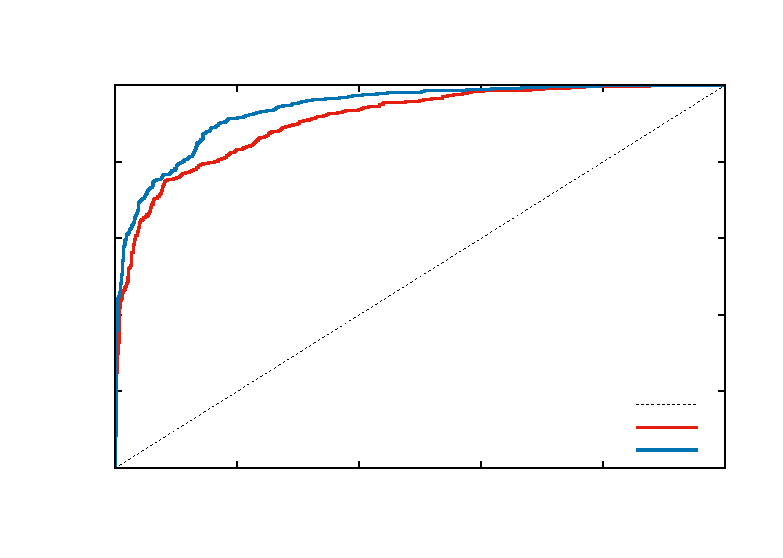
\includegraphics{figs/roc_1}}%
    \gplfronttext
  \end{picture}%
\endgroup
}}

\subfloat[\emph{Full GMHMM}]{\resizebox{\linewidth}{!}{% GNUPLOT: LaTeX picture with Postscript
\begingroup
  \makeatletter
  \providecommand\color[2][]{%
    \GenericError{(gnuplot) \space\space\space\@spaces}{%
      Package color not loaded in conjunction with
      terminal option `colourtext'%
    }{See the gnuplot documentation for explanation.%
    }{Either use 'blacktext' in gnuplot or load the package
      color.sty in LaTeX.}%
    \renewcommand\color[2][]{}%
  }%
  \providecommand\includegraphics[2][]{%
    \GenericError{(gnuplot) \space\space\space\@spaces}{%
      Package graphicx or graphics not loaded%
    }{See the gnuplot documentation for explanation.%
    }{The gnuplot epslatex terminal needs graphicx.sty or graphics.sty.}%
    \renewcommand\includegraphics[2][]{}%
  }%
  \providecommand\rotatebox[2]{#2}%
  \@ifundefined{ifGPcolor}{%
    \newif\ifGPcolor
    \GPcolortrue
  }{}%
  \@ifundefined{ifGPblacktext}{%
    \newif\ifGPblacktext
    \GPblacktextfalse
  }{}%
  % define a \g@addto@macro without @ in the name:
  \let\gplgaddtomacro\g@addto@macro
  % define empty templates for all commands taking text:
  \gdef\gplbacktext{}%
  \gdef\gplfronttext{}%
  \makeatother
  \ifGPblacktext
    % no textcolor at all
    \def\colorrgb#1{}%
    \def\colorgray#1{}%
  \else
    % gray or color?
    \ifGPcolor
      \def\colorrgb#1{\color[rgb]{#1}}%
      \def\colorgray#1{\color[gray]{#1}}%
      \expandafter\def\csname LTw\endcsname{\color{white}}%
      \expandafter\def\csname LTb\endcsname{\color{black}}%
      \expandafter\def\csname LTa\endcsname{\color{black}}%
      \expandafter\def\csname LT0\endcsname{\color[rgb]{1,0,0}}%
      \expandafter\def\csname LT1\endcsname{\color[rgb]{0,1,0}}%
      \expandafter\def\csname LT2\endcsname{\color[rgb]{0,0,1}}%
      \expandafter\def\csname LT3\endcsname{\color[rgb]{1,0,1}}%
      \expandafter\def\csname LT4\endcsname{\color[rgb]{0,1,1}}%
      \expandafter\def\csname LT5\endcsname{\color[rgb]{1,1,0}}%
      \expandafter\def\csname LT6\endcsname{\color[rgb]{0,0,0}}%
      \expandafter\def\csname LT7\endcsname{\color[rgb]{1,0.3,0}}%
      \expandafter\def\csname LT8\endcsname{\color[rgb]{0.5,0.5,0.5}}%
    \else
      % gray
      \def\colorrgb#1{\color{black}}%
      \def\colorgray#1{\color[gray]{#1}}%
      \expandafter\def\csname LTw\endcsname{\color{white}}%
      \expandafter\def\csname LTb\endcsname{\color{black}}%
      \expandafter\def\csname LTa\endcsname{\color{black}}%
      \expandafter\def\csname LT0\endcsname{\color{black}}%
      \expandafter\def\csname LT1\endcsname{\color{black}}%
      \expandafter\def\csname LT2\endcsname{\color{black}}%
      \expandafter\def\csname LT3\endcsname{\color{black}}%
      \expandafter\def\csname LT4\endcsname{\color{black}}%
      \expandafter\def\csname LT5\endcsname{\color{black}}%
      \expandafter\def\csname LT6\endcsname{\color{black}}%
      \expandafter\def\csname LT7\endcsname{\color{black}}%
      \expandafter\def\csname LT8\endcsname{\color{black}}%
    \fi
  \fi
    \setlength{\unitlength}{0.0500bp}%
    \ifx\gptboxheight\undefined%
      \newlength{\gptboxheight}%
      \newlength{\gptboxwidth}%
      \newsavebox{\gptboxtext}%
    \fi%
    \setlength{\fboxrule}{0.5pt}%
    \setlength{\fboxsep}{1pt}%
\begin{picture}(7200.00,5040.00)%
    \gplgaddtomacro\gplbacktext{%
      \csname LTb\endcsname%
      \put(814,704){\makebox(0,0)[r]{\strut{}0}}%
      \put(814,1439){\makebox(0,0)[r]{\strut{}0.2}}%
      \put(814,2174){\makebox(0,0)[r]{\strut{}0.4}}%
      \put(814,2909){\makebox(0,0)[r]{\strut{}0.6}}%
      \put(814,3644){\makebox(0,0)[r]{\strut{}0.8}}%
      \put(814,4379){\makebox(0,0)[r]{\strut{}1}}%
      \put(946,484){\makebox(0,0){\strut{}0}}%
      \put(2117,484){\makebox(0,0){\strut{}0.2}}%
      \put(3289,484){\makebox(0,0){\strut{}0.4}}%
      \put(4460,484){\makebox(0,0){\strut{}0.6}}%
      \put(5632,484){\makebox(0,0){\strut{}0.8}}%
      \put(6803,484){\makebox(0,0){\strut{}1}}%
      \put(3875,1623){\makebox(0,0)[l]{\strut{}Paired $t$-test: $p = 0.0139$}}%
    }%
    \gplgaddtomacro\gplfronttext{%
      \csname LTb\endcsname%
      \put(176,2541){\rotatebox{-270}{\makebox(0,0){\strut{}True positive rate}}}%
      \put(3874,154){\makebox(0,0){\strut{}False positive rate}}%
      \put(3874,4709){\makebox(0,0){\strut{}\bf Full GMHMM: Mean ROC curves after 10-fold crossvalidation}}%
      \csname LTb\endcsname%
      \put(5816,1317){\makebox(0,0)[r]{\strut{}\footnotesize random (area = 0.5)}}%
      \csname LTb\endcsname%
      \put(5816,1097){\makebox(0,0)[r]{\strut{}\footnotesize gmhmm (area = 0.914)}}%
      \csname LTb\endcsname%
      \put(5816,877){\makebox(0,0)[r]{\strut{}\footnotesize multiplex (area = {\bf 0.926})}}%
    }%
    \gplbacktext
    \put(0,0){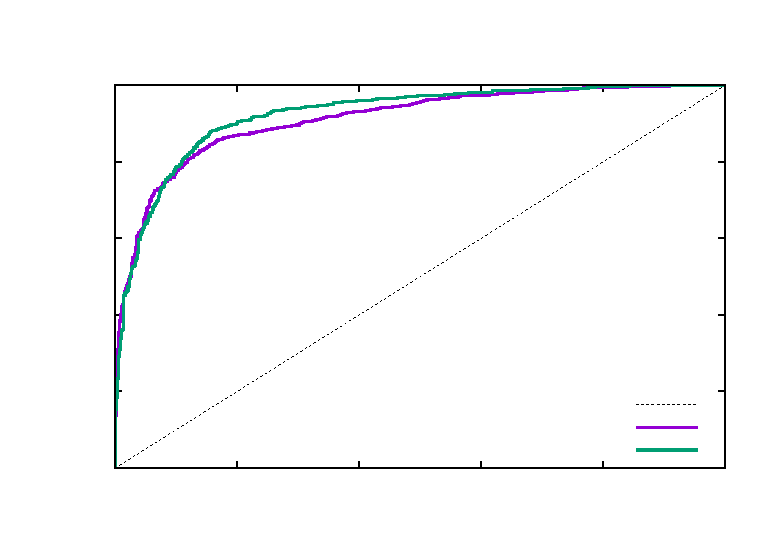
\includegraphics{figs/roc_2}}%
    \gplfronttext
  \end{picture}%
\endgroup
}}
\caption{Mean ROC curves for the implemented models on synthetic data.}\label{figrocsyn1}
\end{figure}
%\begin{figure}\centering
%\resizebox{0.9\linewidth}{!}{% GNUPLOT: LaTeX picture with Postscript
\begingroup
  \makeatletter
  \providecommand\color[2][]{%
    \GenericError{(gnuplot) \space\space\space\@spaces}{%
      Package color not loaded in conjunction with
      terminal option `colourtext'%
    }{See the gnuplot documentation for explanation.%
    }{Either use 'blacktext' in gnuplot or load the package
      color.sty in LaTeX.}%
    \renewcommand\color[2][]{}%
  }%
  \providecommand\includegraphics[2][]{%
    \GenericError{(gnuplot) \space\space\space\@spaces}{%
      Package graphicx or graphics not loaded%
    }{See the gnuplot documentation for explanation.%
    }{The gnuplot epslatex terminal needs graphicx.sty or graphics.sty.}%
    \renewcommand\includegraphics[2][]{}%
  }%
  \providecommand\rotatebox[2]{#2}%
  \@ifundefined{ifGPcolor}{%
    \newif\ifGPcolor
    \GPcolortrue
  }{}%
  \@ifundefined{ifGPblacktext}{%
    \newif\ifGPblacktext
    \GPblacktextfalse
  }{}%
  % define a \g@addto@macro without @ in the name:
  \let\gplgaddtomacro\g@addto@macro
  % define empty templates for all commands taking text:
  \gdef\gplbacktext{}%
  \gdef\gplfronttext{}%
  \makeatother
  \ifGPblacktext
    % no textcolor at all
    \def\colorrgb#1{}%
    \def\colorgray#1{}%
  \else
    % gray or color?
    \ifGPcolor
      \def\colorrgb#1{\color[rgb]{#1}}%
      \def\colorgray#1{\color[gray]{#1}}%
      \expandafter\def\csname LTw\endcsname{\color{white}}%
      \expandafter\def\csname LTb\endcsname{\color{black}}%
      \expandafter\def\csname LTa\endcsname{\color{black}}%
      \expandafter\def\csname LT0\endcsname{\color[rgb]{1,0,0}}%
      \expandafter\def\csname LT1\endcsname{\color[rgb]{0,1,0}}%
      \expandafter\def\csname LT2\endcsname{\color[rgb]{0,0,1}}%
      \expandafter\def\csname LT3\endcsname{\color[rgb]{1,0,1}}%
      \expandafter\def\csname LT4\endcsname{\color[rgb]{0,1,1}}%
      \expandafter\def\csname LT5\endcsname{\color[rgb]{1,1,0}}%
      \expandafter\def\csname LT6\endcsname{\color[rgb]{0,0,0}}%
      \expandafter\def\csname LT7\endcsname{\color[rgb]{1,0.3,0}}%
      \expandafter\def\csname LT8\endcsname{\color[rgb]{0.5,0.5,0.5}}%
    \else
      % gray
      \def\colorrgb#1{\color{black}}%
      \def\colorgray#1{\color[gray]{#1}}%
      \expandafter\def\csname LTw\endcsname{\color{white}}%
      \expandafter\def\csname LTb\endcsname{\color{black}}%
      \expandafter\def\csname LTa\endcsname{\color{black}}%
      \expandafter\def\csname LT0\endcsname{\color{black}}%
      \expandafter\def\csname LT1\endcsname{\color{black}}%
      \expandafter\def\csname LT2\endcsname{\color{black}}%
      \expandafter\def\csname LT3\endcsname{\color{black}}%
      \expandafter\def\csname LT4\endcsname{\color{black}}%
      \expandafter\def\csname LT5\endcsname{\color{black}}%
      \expandafter\def\csname LT6\endcsname{\color{black}}%
      \expandafter\def\csname LT7\endcsname{\color{black}}%
      \expandafter\def\csname LT8\endcsname{\color{black}}%
    \fi
  \fi
    \setlength{\unitlength}{0.0500bp}%
    \ifx\gptboxheight\undefined%
      \newlength{\gptboxheight}%
      \newlength{\gptboxwidth}%
      \newsavebox{\gptboxtext}%
    \fi%
    \setlength{\fboxrule}{0.5pt}%
    \setlength{\fboxsep}{1pt}%
\begin{picture}(7200.00,5040.00)%
    \gplgaddtomacro\gplbacktext{%
      \csname LTb\endcsname%
      \put(814,704){\makebox(0,0)[r]{\strut{}0}}%
      \put(814,1439){\makebox(0,0)[r]{\strut{}0.2}}%
      \put(814,2174){\makebox(0,0)[r]{\strut{}0.4}}%
      \put(814,2909){\makebox(0,0)[r]{\strut{}0.6}}%
      \put(814,3644){\makebox(0,0)[r]{\strut{}0.8}}%
      \put(814,4379){\makebox(0,0)[r]{\strut{}1}}%
      \put(946,484){\makebox(0,0){\strut{}0}}%
      \put(2117,484){\makebox(0,0){\strut{}0.2}}%
      \put(3289,484){\makebox(0,0){\strut{}0.4}}%
      \put(4460,484){\makebox(0,0){\strut{}0.6}}%
      \put(5632,484){\makebox(0,0){\strut{}0.8}}%
      \put(6803,484){\makebox(0,0){\strut{}1}}%
      \put(3875,1623){\makebox(0,0)[l]{\strut{}Paired $t$-test: $p = 0.0139$}}%
    }%
    \gplgaddtomacro\gplfronttext{%
      \csname LTb\endcsname%
      \put(176,2541){\rotatebox{-270}{\makebox(0,0){\strut{}True positive rate}}}%
      \put(3874,154){\makebox(0,0){\strut{}False positive rate}}%
      \put(3874,4709){\makebox(0,0){\strut{}\bf Full GMHMM: Mean ROC curves after 10-fold crossvalidation}}%
      \csname LTb\endcsname%
      \put(5816,1317){\makebox(0,0)[r]{\strut{}\footnotesize random (area = 0.5)}}%
      \csname LTb\endcsname%
      \put(5816,1097){\makebox(0,0)[r]{\strut{}\footnotesize gmhmm (area = 0.914)}}%
      \csname LTb\endcsname%
      \put(5816,877){\makebox(0,0)[r]{\strut{}\footnotesize multiplex (area = {\bf 0.926})}}%
    }%
    \gplbacktext
    \put(0,0){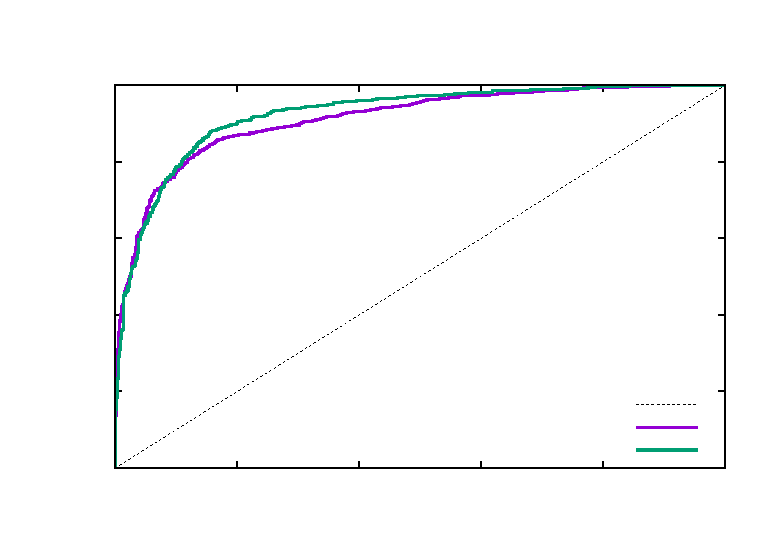
\includegraphics{figs/roc_2}}%
    \gplfronttext
  \end{picture}%
\endgroup
}
%\caption{Mean ROC curves for the full GMHMM models ran on synthetic data.}\label{figrocsyn2}
%\end{figure}

\noindent These results successfully demonstrate that, as expected, \textbf{the multiplex models outperform their monoplex counterparts} on each of the metrics considered---and all but two of those performance gains are statistically significant ($p < 0.01$). The decrease in significance for the full GMHMM may be explained by the fact that, as the data is normally distributed, there is bound to be a set of data points that will be offset incorrectly, and hence end up being classified to the other class, no matter how well the classifier is trained. The full GMHMM already manages to approach those limits on its own, and thus the multiplex GMHMM is not able to give as significant comparative benefits as the chain multiplex (however the improvements are still noticeable).\\ \\
Lastly, it might be useful to compare the two monoplex and multiplex models against one another. The results of this comparison are summarised in Table \ref{tblsyndata3}.\\ \\
The full GMHMM outperforms the chain GMHMM with statistical significance in almost all metrics, which is expected due to the larger expressivity of the full GMHMM. The observed differences in their multiplex counterparts, however, have been shown to be largely statistically insignificant, which is consistent with both models approaching the previously mentioned limits imposed by the data's underlying distribution.
\begin{table}[h]\centering
\begin{tabular}{ l c c r } \toprule
{\bf Parameter} & {\bf Monoplex models} & {\bf Multiplex models} \\ \midrule
Accuracy & $p = \underline{0.0013}$ & $p = 0.2339$ \\
Sensitivity & $p = 0.0166$ & $p = 0.5000$ \\
MCC & $p = \underline{0.0011}$ & $p = 0.3192$ \\
$F_1$ score & $p = \underline{0.0012}$ & $p = 0.3059$ \\
Area under ROC curve & $p = \underline{0.0073}$ & $p = \underline{0.0021}$\\
\bottomrule
\end{tabular}
\caption[Evaluation results on the chain GMHMM on synthetic data]{\centering Statistical significance of the observed differences in the monoplex and multiplex models separately, on synthetic data.}\label{tblsyndata3}
\end{table}

\subsection{Biomolecular data}\label{secBiomoldata}

Satisfied that the models operate as expected on the controlled data set, I moved on to evaluating the same performance metrics as before on a real data set.\\ \\
The main problem tackled here is classification of subjects for \emph{breast invasive carcinoma (BRCA)}, based on the activity metrics for the genes in the tumour necrosis factor receptor superfamily (TNFRSF). These genes are responsible for production of receptors that are able to bind to tumour necrosis factors (TNFs), proteins capable of inducing cell death (apoptosis) of tumourous cells, and as such, their activity levels are expected to be correlated with the incidence of specific cancers. The particular genetic activity metrics considered as the two principal data types are \emph{gene expression} and \emph{methylation}.\\ \\
The data set utilised has been obtained from the \emph{Cancer Genome Atlas (TCGA)}\footnote{\url{https://tcga-data.nci.nih.gov/tcga/}} and contains expression and methylation measurements for 26 genes in the TNFRSF; there are $776$ patient and $79$ normal samples in the data set. To translate this data into the GMHMM terminology, each gene corresponds to a single sub-output, and a single subject's sequence is fed into the models such that the more active genes come first (here I have used the \emph{euclidean norm} of a gene's data point as its activity measure; $activity(g) = \sqrt{expression_g^2 + methylation_g^2}$).\\ \\
The results of the comparative evaluation after 10-fold crossvalidation on this data set are summarised in Tables \ref{tblbiodata1} and \ref{tblbiodata2} as well as in Figure \ref{figrocbio1}.% and \ref{figrocbio2}.

\begin{table}[h]\centering
\begin{tabular}{ l c c r } \toprule
{\bf Parameter} & {\bf Chain GMHMM} & {\bf Multiplex chain GMHMM} & {\bf $p$-value} \\ \midrule
Accuracy & $0.898296$ & $\bf 0.944091$ & $\underline{0.000063}$\\
Sensitivity & $0.890239$ & $\bf 0.984906$ & $\underline{0.000003}$\\
MCC & $\bf 0.665473$ & $0.663314$ & $0.483599$\\
$F_1$ score & $0.939568$ & $\bf 0.969341$ & $\underline{0.000039}$\\
\bottomrule
\end{tabular}
\caption[Evaluation results on the chain GMHMM on synthetic data]{\centering Comparative evaluation results of the chain GMHMMs on biomolecular data.}\label{tblbiodata1}
\end{table}
\begin{table}[h]\centering
\begin{tabular}{ l c c r } \toprule
{\bf Parameter} & {\bf Full GMHMM} & {\bf Full multiplex GMHMM} & {\bf $p$-value} \\ \midrule
Accuracy & $0.935643$ & $\bf 0.9424548$ & $0.3299$\\
Sensitivity & $0.941292$ & $\bf 0.9584906$ & $0.2474$\\
MCC & $0.734150$ & $\bf 0.7500727$ & $0.3130$\\
$F_1$ score & $0.962836$ & $\bf 0.9669872$ & $0.3329$\\
\bottomrule
\end{tabular}
\caption[Evaluation results on the full GMHMMs on biomolecular data]{\centering Comparative evaluation results of the full GMHMM models\linebreak on biomolecular data.}\label{tblbiodata2}
\end{table}
\begin{figure}[p]\centering
\subfloat[\emph{Chain GMHMM}]{\resizebox{\linewidth}{!}{% GNUPLOT: LaTeX picture with Postscript
\begingroup
  \makeatletter
  \providecommand\color[2][]{%
    \GenericError{(gnuplot) \space\space\space\@spaces}{%
      Package color not loaded in conjunction with
      terminal option `colourtext'%
    }{See the gnuplot documentation for explanation.%
    }{Either use 'blacktext' in gnuplot or load the package
      color.sty in LaTeX.}%
    \renewcommand\color[2][]{}%
  }%
  \providecommand\includegraphics[2][]{%
    \GenericError{(gnuplot) \space\space\space\@spaces}{%
      Package graphicx or graphics not loaded%
    }{See the gnuplot documentation for explanation.%
    }{The gnuplot epslatex terminal needs graphicx.sty or graphics.sty.}%
    \renewcommand\includegraphics[2][]{}%
  }%
  \providecommand\rotatebox[2]{#2}%
  \@ifundefined{ifGPcolor}{%
    \newif\ifGPcolor
    \GPcolortrue
  }{}%
  \@ifundefined{ifGPblacktext}{%
    \newif\ifGPblacktext
    \GPblacktextfalse
  }{}%
  % define a \g@addto@macro without @ in the name:
  \let\gplgaddtomacro\g@addto@macro
  % define empty templates for all commands taking text:
  \gdef\gplbacktext{}%
  \gdef\gplfronttext{}%
  \makeatother
  \ifGPblacktext
    % no textcolor at all
    \def\colorrgb#1{}%
    \def\colorgray#1{}%
  \else
    % gray or color?
    \ifGPcolor
      \def\colorrgb#1{\color[rgb]{#1}}%
      \def\colorgray#1{\color[gray]{#1}}%
      \expandafter\def\csname LTw\endcsname{\color{white}}%
      \expandafter\def\csname LTb\endcsname{\color{black}}%
      \expandafter\def\csname LTa\endcsname{\color{black}}%
      \expandafter\def\csname LT0\endcsname{\color[rgb]{1,0,0}}%
      \expandafter\def\csname LT1\endcsname{\color[rgb]{0,1,0}}%
      \expandafter\def\csname LT2\endcsname{\color[rgb]{0,0,1}}%
      \expandafter\def\csname LT3\endcsname{\color[rgb]{1,0,1}}%
      \expandafter\def\csname LT4\endcsname{\color[rgb]{0,1,1}}%
      \expandafter\def\csname LT5\endcsname{\color[rgb]{1,1,0}}%
      \expandafter\def\csname LT6\endcsname{\color[rgb]{0,0,0}}%
      \expandafter\def\csname LT7\endcsname{\color[rgb]{1,0.3,0}}%
      \expandafter\def\csname LT8\endcsname{\color[rgb]{0.5,0.5,0.5}}%
    \else
      % gray
      \def\colorrgb#1{\color{black}}%
      \def\colorgray#1{\color[gray]{#1}}%
      \expandafter\def\csname LTw\endcsname{\color{white}}%
      \expandafter\def\csname LTb\endcsname{\color{black}}%
      \expandafter\def\csname LTa\endcsname{\color{black}}%
      \expandafter\def\csname LT0\endcsname{\color{black}}%
      \expandafter\def\csname LT1\endcsname{\color{black}}%
      \expandafter\def\csname LT2\endcsname{\color{black}}%
      \expandafter\def\csname LT3\endcsname{\color{black}}%
      \expandafter\def\csname LT4\endcsname{\color{black}}%
      \expandafter\def\csname LT5\endcsname{\color{black}}%
      \expandafter\def\csname LT6\endcsname{\color{black}}%
      \expandafter\def\csname LT7\endcsname{\color{black}}%
      \expandafter\def\csname LT8\endcsname{\color{black}}%
    \fi
  \fi
    \setlength{\unitlength}{0.0500bp}%
    \ifx\gptboxheight\undefined%
      \newlength{\gptboxheight}%
      \newlength{\gptboxwidth}%
      \newsavebox{\gptboxtext}%
    \fi%
    \setlength{\fboxrule}{0.5pt}%
    \setlength{\fboxsep}{1pt}%
\begin{picture}(7200.00,5040.00)%
    \gplgaddtomacro\gplbacktext{%
      \csname LTb\endcsname%
      \put(814,704){\makebox(0,0)[r]{\strut{}0}}%
      \put(814,1439){\makebox(0,0)[r]{\strut{}0.2}}%
      \put(814,2174){\makebox(0,0)[r]{\strut{}0.4}}%
      \put(814,2909){\makebox(0,0)[r]{\strut{}0.6}}%
      \put(814,3644){\makebox(0,0)[r]{\strut{}0.8}}%
      \put(814,4379){\makebox(0,0)[r]{\strut{}1}}%
      \put(946,484){\makebox(0,0){\strut{}0}}%
      \put(2117,484){\makebox(0,0){\strut{}0.2}}%
      \put(3289,484){\makebox(0,0){\strut{}0.4}}%
      \put(4460,484){\makebox(0,0){\strut{}0.6}}%
      \put(5632,484){\makebox(0,0){\strut{}0.8}}%
      \put(6803,484){\makebox(0,0){\strut{}1}}%
      \put(3875,1623){\makebox(0,0)[l]{\strut{}Paired t-test: $p = 0.0432$}}%
    }%
    \gplgaddtomacro\gplfronttext{%
      \csname LTb\endcsname%
      \put(176,2541){\rotatebox{-270}{\makebox(0,0){\strut{}True positive rate}}}%
      \put(3874,154){\makebox(0,0){\strut{}False positive rate}}%
      \put(3874,4709){\makebox(0,0){\strut{}\bf Chain GMHMM: Mean ROC curves after 10-fold crossvalidation}}%
      \csname LTb\endcsname%
      \put(5816,1317){\makebox(0,0)[r]{\strut{}\footnotesize random (area = 0.5)}}%
      \csname LTb\endcsname%
      \put(5816,1097){\makebox(0,0)[r]{\strut{}\footnotesize chain (area = {\bf 0.986})}}%
      \csname LTb\endcsname%
      \put(5816,877){\makebox(0,0)[r]{\strut{}\footnotesize multiplex (area =  0.953)}}%
    }%
    \gplbacktext
    \put(0,0){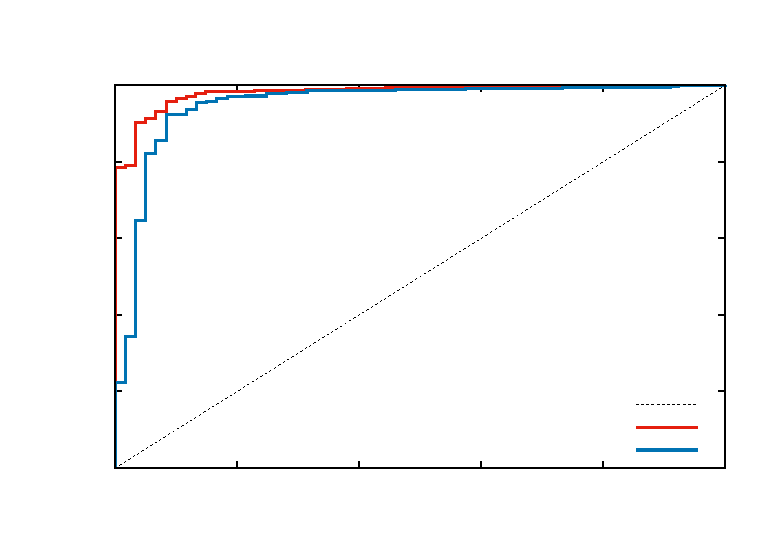
\includegraphics{figs/roc_3}}%
    \gplfronttext
  \end{picture}%
\endgroup
}}

\subfloat[\emph{Full GMHMM}]{\resizebox{\linewidth}{!}{% GNUPLOT: LaTeX picture with Postscript
\begingroup
  \makeatletter
  \providecommand\color[2][]{%
    \GenericError{(gnuplot) \space\space\space\@spaces}{%
      Package color not loaded in conjunction with
      terminal option `colourtext'%
    }{See the gnuplot documentation for explanation.%
    }{Either use 'blacktext' in gnuplot or load the package
      color.sty in LaTeX.}%
    \renewcommand\color[2][]{}%
  }%
  \providecommand\includegraphics[2][]{%
    \GenericError{(gnuplot) \space\space\space\@spaces}{%
      Package graphicx or graphics not loaded%
    }{See the gnuplot documentation for explanation.%
    }{The gnuplot epslatex terminal needs graphicx.sty or graphics.sty.}%
    \renewcommand\includegraphics[2][]{}%
  }%
  \providecommand\rotatebox[2]{#2}%
  \@ifundefined{ifGPcolor}{%
    \newif\ifGPcolor
    \GPcolortrue
  }{}%
  \@ifundefined{ifGPblacktext}{%
    \newif\ifGPblacktext
    \GPblacktextfalse
  }{}%
  % define a \g@addto@macro without @ in the name:
  \let\gplgaddtomacro\g@addto@macro
  % define empty templates for all commands taking text:
  \gdef\gplbacktext{}%
  \gdef\gplfronttext{}%
  \makeatother
  \ifGPblacktext
    % no textcolor at all
    \def\colorrgb#1{}%
    \def\colorgray#1{}%
  \else
    % gray or color?
    \ifGPcolor
      \def\colorrgb#1{\color[rgb]{#1}}%
      \def\colorgray#1{\color[gray]{#1}}%
      \expandafter\def\csname LTw\endcsname{\color{white}}%
      \expandafter\def\csname LTb\endcsname{\color{black}}%
      \expandafter\def\csname LTa\endcsname{\color{black}}%
      \expandafter\def\csname LT0\endcsname{\color[rgb]{1,0,0}}%
      \expandafter\def\csname LT1\endcsname{\color[rgb]{0,1,0}}%
      \expandafter\def\csname LT2\endcsname{\color[rgb]{0,0,1}}%
      \expandafter\def\csname LT3\endcsname{\color[rgb]{1,0,1}}%
      \expandafter\def\csname LT4\endcsname{\color[rgb]{0,1,1}}%
      \expandafter\def\csname LT5\endcsname{\color[rgb]{1,1,0}}%
      \expandafter\def\csname LT6\endcsname{\color[rgb]{0,0,0}}%
      \expandafter\def\csname LT7\endcsname{\color[rgb]{1,0.3,0}}%
      \expandafter\def\csname LT8\endcsname{\color[rgb]{0.5,0.5,0.5}}%
    \else
      % gray
      \def\colorrgb#1{\color{black}}%
      \def\colorgray#1{\color[gray]{#1}}%
      \expandafter\def\csname LTw\endcsname{\color{white}}%
      \expandafter\def\csname LTb\endcsname{\color{black}}%
      \expandafter\def\csname LTa\endcsname{\color{black}}%
      \expandafter\def\csname LT0\endcsname{\color{black}}%
      \expandafter\def\csname LT1\endcsname{\color{black}}%
      \expandafter\def\csname LT2\endcsname{\color{black}}%
      \expandafter\def\csname LT3\endcsname{\color{black}}%
      \expandafter\def\csname LT4\endcsname{\color{black}}%
      \expandafter\def\csname LT5\endcsname{\color{black}}%
      \expandafter\def\csname LT6\endcsname{\color{black}}%
      \expandafter\def\csname LT7\endcsname{\color{black}}%
      \expandafter\def\csname LT8\endcsname{\color{black}}%
    \fi
  \fi
    \setlength{\unitlength}{0.0500bp}%
    \ifx\gptboxheight\undefined%
      \newlength{\gptboxheight}%
      \newlength{\gptboxwidth}%
      \newsavebox{\gptboxtext}%
    \fi%
    \setlength{\fboxrule}{0.5pt}%
    \setlength{\fboxsep}{1pt}%
\begin{picture}(7200.00,5040.00)%
    \gplgaddtomacro\gplbacktext{%
      \csname LTb\endcsname%
      \put(814,704){\makebox(0,0)[r]{\strut{}0}}%
      \put(814,1439){\makebox(0,0)[r]{\strut{}0.2}}%
      \put(814,2174){\makebox(0,0)[r]{\strut{}0.4}}%
      \put(814,2909){\makebox(0,0)[r]{\strut{}0.6}}%
      \put(814,3644){\makebox(0,0)[r]{\strut{}0.8}}%
      \put(814,4379){\makebox(0,0)[r]{\strut{}1}}%
      \put(946,484){\makebox(0,0){\strut{}0}}%
      \put(2117,484){\makebox(0,0){\strut{}0.2}}%
      \put(3289,484){\makebox(0,0){\strut{}0.4}}%
      \put(4460,484){\makebox(0,0){\strut{}0.6}}%
      \put(5632,484){\makebox(0,0){\strut{}0.8}}%
      \put(6803,484){\makebox(0,0){\strut{}1}}%
      \put(3875,1623){\makebox(0,0)[l]{\strut{}Paired t-test: $p = 0.0437$}}%
    }%
    \gplgaddtomacro\gplfronttext{%
      \csname LTb\endcsname%
      \put(176,2541){\rotatebox{-270}{\makebox(0,0){\strut{}True positive rate}}}%
      \put(3874,154){\makebox(0,0){\strut{}False positive rate}}%
      \put(3874,4709){\makebox(0,0){\strut{}\bf Full GMHMM: Mean ROC curves after 10-fold crossvalidation}}%
      \csname LTb\endcsname%
      \put(5816,1317){\makebox(0,0)[r]{\strut{}\footnotesize random (area = 0.5)}}%
      \csname LTb\endcsname%
      \put(5816,1097){\makebox(0,0)[r]{\strut{}\footnotesize gmhmm (area = {\bf 0.985})}}%
      \csname LTb\endcsname%
      \put(5816,877){\makebox(0,0)[r]{\strut{}\footnotesize multiplex (area = 0.919)}}%
    }%
    \gplbacktext
    \put(0,0){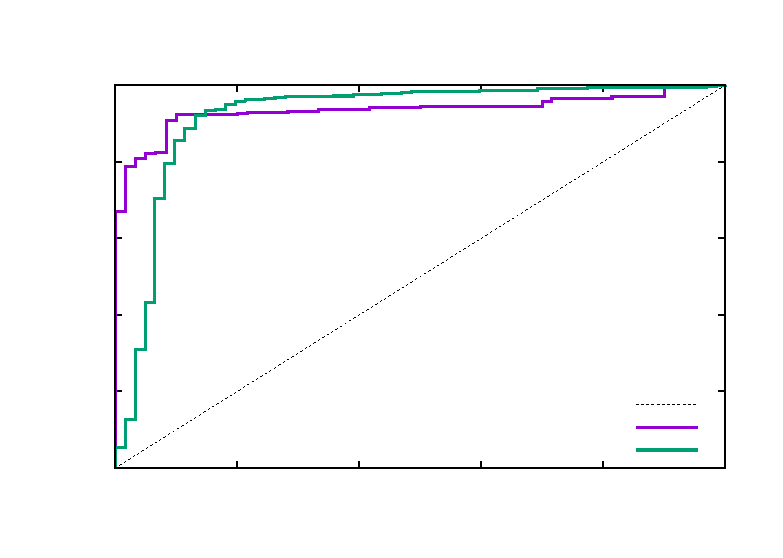
\includegraphics{figs/roc_4}}%
    \gplfronttext
  \end{picture}%
\endgroup
}}
\caption{Mean ROC curves for the implemented models on biomolecular data.}\label{figrocbio1}
\end{figure}
%\begin{figure}[h]\centering
%\resizebox{0.9\linewidth}{!}{% GNUPLOT: LaTeX picture with Postscript
\begingroup
  \makeatletter
  \providecommand\color[2][]{%
    \GenericError{(gnuplot) \space\space\space\@spaces}{%
      Package color not loaded in conjunction with
      terminal option `colourtext'%
    }{See the gnuplot documentation for explanation.%
    }{Either use 'blacktext' in gnuplot or load the package
      color.sty in LaTeX.}%
    \renewcommand\color[2][]{}%
  }%
  \providecommand\includegraphics[2][]{%
    \GenericError{(gnuplot) \space\space\space\@spaces}{%
      Package graphicx or graphics not loaded%
    }{See the gnuplot documentation for explanation.%
    }{The gnuplot epslatex terminal needs graphicx.sty or graphics.sty.}%
    \renewcommand\includegraphics[2][]{}%
  }%
  \providecommand\rotatebox[2]{#2}%
  \@ifundefined{ifGPcolor}{%
    \newif\ifGPcolor
    \GPcolortrue
  }{}%
  \@ifundefined{ifGPblacktext}{%
    \newif\ifGPblacktext
    \GPblacktextfalse
  }{}%
  % define a \g@addto@macro without @ in the name:
  \let\gplgaddtomacro\g@addto@macro
  % define empty templates for all commands taking text:
  \gdef\gplbacktext{}%
  \gdef\gplfronttext{}%
  \makeatother
  \ifGPblacktext
    % no textcolor at all
    \def\colorrgb#1{}%
    \def\colorgray#1{}%
  \else
    % gray or color?
    \ifGPcolor
      \def\colorrgb#1{\color[rgb]{#1}}%
      \def\colorgray#1{\color[gray]{#1}}%
      \expandafter\def\csname LTw\endcsname{\color{white}}%
      \expandafter\def\csname LTb\endcsname{\color{black}}%
      \expandafter\def\csname LTa\endcsname{\color{black}}%
      \expandafter\def\csname LT0\endcsname{\color[rgb]{1,0,0}}%
      \expandafter\def\csname LT1\endcsname{\color[rgb]{0,1,0}}%
      \expandafter\def\csname LT2\endcsname{\color[rgb]{0,0,1}}%
      \expandafter\def\csname LT3\endcsname{\color[rgb]{1,0,1}}%
      \expandafter\def\csname LT4\endcsname{\color[rgb]{0,1,1}}%
      \expandafter\def\csname LT5\endcsname{\color[rgb]{1,1,0}}%
      \expandafter\def\csname LT6\endcsname{\color[rgb]{0,0,0}}%
      \expandafter\def\csname LT7\endcsname{\color[rgb]{1,0.3,0}}%
      \expandafter\def\csname LT8\endcsname{\color[rgb]{0.5,0.5,0.5}}%
    \else
      % gray
      \def\colorrgb#1{\color{black}}%
      \def\colorgray#1{\color[gray]{#1}}%
      \expandafter\def\csname LTw\endcsname{\color{white}}%
      \expandafter\def\csname LTb\endcsname{\color{black}}%
      \expandafter\def\csname LTa\endcsname{\color{black}}%
      \expandafter\def\csname LT0\endcsname{\color{black}}%
      \expandafter\def\csname LT1\endcsname{\color{black}}%
      \expandafter\def\csname LT2\endcsname{\color{black}}%
      \expandafter\def\csname LT3\endcsname{\color{black}}%
      \expandafter\def\csname LT4\endcsname{\color{black}}%
      \expandafter\def\csname LT5\endcsname{\color{black}}%
      \expandafter\def\csname LT6\endcsname{\color{black}}%
      \expandafter\def\csname LT7\endcsname{\color{black}}%
      \expandafter\def\csname LT8\endcsname{\color{black}}%
    \fi
  \fi
    \setlength{\unitlength}{0.0500bp}%
    \ifx\gptboxheight\undefined%
      \newlength{\gptboxheight}%
      \newlength{\gptboxwidth}%
      \newsavebox{\gptboxtext}%
    \fi%
    \setlength{\fboxrule}{0.5pt}%
    \setlength{\fboxsep}{1pt}%
\begin{picture}(7200.00,5040.00)%
    \gplgaddtomacro\gplbacktext{%
      \csname LTb\endcsname%
      \put(814,704){\makebox(0,0)[r]{\strut{}0}}%
      \put(814,1439){\makebox(0,0)[r]{\strut{}0.2}}%
      \put(814,2174){\makebox(0,0)[r]{\strut{}0.4}}%
      \put(814,2909){\makebox(0,0)[r]{\strut{}0.6}}%
      \put(814,3644){\makebox(0,0)[r]{\strut{}0.8}}%
      \put(814,4379){\makebox(0,0)[r]{\strut{}1}}%
      \put(946,484){\makebox(0,0){\strut{}0}}%
      \put(2117,484){\makebox(0,0){\strut{}0.2}}%
      \put(3289,484){\makebox(0,0){\strut{}0.4}}%
      \put(4460,484){\makebox(0,0){\strut{}0.6}}%
      \put(5632,484){\makebox(0,0){\strut{}0.8}}%
      \put(6803,484){\makebox(0,0){\strut{}1}}%
      \put(3875,1623){\makebox(0,0)[l]{\strut{}Paired t-test: $p = 0.0437$}}%
    }%
    \gplgaddtomacro\gplfronttext{%
      \csname LTb\endcsname%
      \put(176,2541){\rotatebox{-270}{\makebox(0,0){\strut{}True positive rate}}}%
      \put(3874,154){\makebox(0,0){\strut{}False positive rate}}%
      \put(3874,4709){\makebox(0,0){\strut{}\bf Full GMHMM: Mean ROC curves after 10-fold crossvalidation}}%
      \csname LTb\endcsname%
      \put(5816,1317){\makebox(0,0)[r]{\strut{}\footnotesize random (area = 0.5)}}%
      \csname LTb\endcsname%
      \put(5816,1097){\makebox(0,0)[r]{\strut{}\footnotesize gmhmm (area = {\bf 0.985})}}%
      \csname LTb\endcsname%
      \put(5816,877){\makebox(0,0)[r]{\strut{}\footnotesize multiplex (area = 0.919)}}%
    }%
    \gplbacktext
    \put(0,0){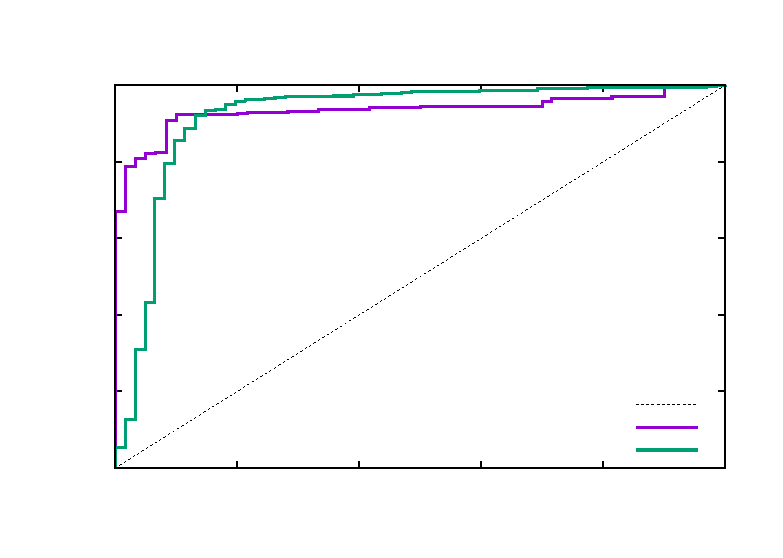
\includegraphics{figs/roc_4}}%
    \gplfronttext
  \end{picture}%
\endgroup
}
%\caption{Mean ROC curves for the full GMHMM models ran on biomolecular data.}\label{figrocbio2}
%\end{figure}
\noindent These results once again demonstrate that, as expected, \textbf{the multiplex models outperform their monoplex counterparts} on most of the metrics considered. The exceptions are the MCC in the chain GMHMM case, as well as the area under the ROC curves in both cases. The decrease in the ROC curve integral is consistent with the formula used to discriminate the solutions returned by NSGA-II (given in \cref{sectrainmuxchn}), as it gives preference to having more sequences with sufficient likelihoods, rather than fewer sequences with very high likelihoods.\\ \\
All the positive differences observed for the chain GMHMM models are statistically \emph{highly significant}; the differences observed for the full GMHMM, while evident, are not statistically significant. This could once again be explained by the fact that the monoplex GMHMM classifier is already able to achieve very high performance on the given data (in several testing sets, \emph{perfect classification} was observed), and therefore it is very hard to make a significant improvement. While outside of the scope of the goals of this project, this likely also demonstrates that the models I have implemented may be \textbf{highly suitable} for handling diagnostics problems such as this one.\\ \\
The statistical significances of the differences observed between each the monoplex and multiplex models separately are given in Table \ref{tblbiodata3}.
\begin{table}[h]\centering
\begin{tabular}{ l c c r } \toprule
{\bf Parameter} & {\bf Monoplex models} & {\bf Multiplex models} \\ \midrule
Accuracy & $p = \underline{0.0081}$ & $p = 0.4606$ \\
Sensitivity & $p = \underline{0.0009}$ & $p = 0.1129$ \\
MCC & $p = 0.0589$ & $p = 0.3192$ \\
$F_1$ score & $p = \underline{0.0070}$ & $p = 0.4049$ \\
Area under ROC curve & $p = 0.4534$ & $p = 0.2092$\\
\bottomrule
\end{tabular}
\caption[Evaluation results on the chain GMHMM on synthetic data]{\centering Statistical significance of the observed differences in the monoplex and multiplex models separately, on biomolecular data.}\label{tblbiodata3}
\end{table}
\noindent The significances obtained from Table \ref{tblbiodata3} further emphasise the \emph{relative power} of the implemented models; the chain GMHMM is already a powerful model for this problem, and it is significantly outperformed by all of the other three models, that cannot be distinguished from one another with statistical significance---implying that it is possible that all of them have reached the potential ``limits'' imposed by the data in the data set.

\section{Robustness analysis}\label{secnojz}

When dealing with real data sets, all the observations presented to the learning algorithms are necessarily accompanied with a certain experimental error, and it is crucial that the learning algorithm is, to a certain extent, capable of \emph{discriminating the noise} from the actual data to be learned.\\ \\
The findings from \cref{secBiomoldata} indicate that the models seem to perform rather well in the presence of any experimental errors that were present in the biomolecular data. To strengthen this indication, I have extended my evaluation suite with a simple \emph{noise testing} facility, which is capable of introducing Gaussian noise (with a specified mean $\mu_n$ and standard deviation $\sigma_n$) into a data set before starting the crossvalidation run.\\ \\
To be able to assess the robustness of the implemented models, I have used a synthetically generated data set with similar characteristics as the one described in \cref{secsyndata}, and recorded the accuracy of the models as the noise's standard deviation increases from $0$ to $2$, in increments of $0.1$ (the mean of the noise was held at zero throughout the experiment). For each noise distribution, the sample mean of \emph{ten 10-fold crossvalidation runs} was used as the final result.\\ \\
The results of the analysis are presented in Figure \ref{fignoise1}.% and \ref{fignoise2}.
\begin{figure}[p]\centering
\subfloat[\emph{Chain GMHMM}]{\resizebox{\linewidth}{!}{% GNUPLOT: LaTeX picture with Postscript
\begingroup
  \makeatletter
  \providecommand\color[2][]{%
    \GenericError{(gnuplot) \space\space\space\@spaces}{%
      Package color not loaded in conjunction with
      terminal option `colourtext'%
    }{See the gnuplot documentation for explanation.%
    }{Either use 'blacktext' in gnuplot or load the package
      color.sty in LaTeX.}%
    \renewcommand\color[2][]{}%
  }%
  \providecommand\includegraphics[2][]{%
    \GenericError{(gnuplot) \space\space\space\@spaces}{%
      Package graphicx or graphics not loaded%
    }{See the gnuplot documentation for explanation.%
    }{The gnuplot epslatex terminal needs graphicx.sty or graphics.sty.}%
    \renewcommand\includegraphics[2][]{}%
  }%
  \providecommand\rotatebox[2]{#2}%
  \@ifundefined{ifGPcolor}{%
    \newif\ifGPcolor
    \GPcolortrue
  }{}%
  \@ifundefined{ifGPblacktext}{%
    \newif\ifGPblacktext
    \GPblacktextfalse
  }{}%
  % define a \g@addto@macro without @ in the name:
  \let\gplgaddtomacro\g@addto@macro
  % define empty templates for all commands taking text:
  \gdef\gplbacktext{}%
  \gdef\gplfronttext{}%
  \makeatother
  \ifGPblacktext
    % no textcolor at all
    \def\colorrgb#1{}%
    \def\colorgray#1{}%
  \else
    % gray or color?
    \ifGPcolor
      \def\colorrgb#1{\color[rgb]{#1}}%
      \def\colorgray#1{\color[gray]{#1}}%
      \expandafter\def\csname LTw\endcsname{\color{white}}%
      \expandafter\def\csname LTb\endcsname{\color{black}}%
      \expandafter\def\csname LTa\endcsname{\color{black}}%
      \expandafter\def\csname LT0\endcsname{\color[rgb]{1,0,0}}%
      \expandafter\def\csname LT1\endcsname{\color[rgb]{0,1,0}}%
      \expandafter\def\csname LT2\endcsname{\color[rgb]{0,0,1}}%
      \expandafter\def\csname LT3\endcsname{\color[rgb]{1,0,1}}%
      \expandafter\def\csname LT4\endcsname{\color[rgb]{0,1,1}}%
      \expandafter\def\csname LT5\endcsname{\color[rgb]{1,1,0}}%
      \expandafter\def\csname LT6\endcsname{\color[rgb]{0,0,0}}%
      \expandafter\def\csname LT7\endcsname{\color[rgb]{1,0.3,0}}%
      \expandafter\def\csname LT8\endcsname{\color[rgb]{0.5,0.5,0.5}}%
    \else
      % gray
      \def\colorrgb#1{\color{black}}%
      \def\colorgray#1{\color[gray]{#1}}%
      \expandafter\def\csname LTw\endcsname{\color{white}}%
      \expandafter\def\csname LTb\endcsname{\color{black}}%
      \expandafter\def\csname LTa\endcsname{\color{black}}%
      \expandafter\def\csname LT0\endcsname{\color{black}}%
      \expandafter\def\csname LT1\endcsname{\color{black}}%
      \expandafter\def\csname LT2\endcsname{\color{black}}%
      \expandafter\def\csname LT3\endcsname{\color{black}}%
      \expandafter\def\csname LT4\endcsname{\color{black}}%
      \expandafter\def\csname LT5\endcsname{\color{black}}%
      \expandafter\def\csname LT6\endcsname{\color{black}}%
      \expandafter\def\csname LT7\endcsname{\color{black}}%
      \expandafter\def\csname LT8\endcsname{\color{black}}%
    \fi
  \fi
    \setlength{\unitlength}{0.0500bp}%
    \ifx\gptboxheight\undefined%
      \newlength{\gptboxheight}%
      \newlength{\gptboxwidth}%
      \newsavebox{\gptboxtext}%
    \fi%
    \setlength{\fboxrule}{0.5pt}%
    \setlength{\fboxsep}{1pt}%
\begin{picture}(7200.00,5040.00)%
    \gplgaddtomacro\gplbacktext{%
      \csname LTb\endcsname%
      \put(946,704){\makebox(0,0)[r]{\strut{}0.6}}%
      \put(946,1317){\makebox(0,0)[r]{\strut{}0.65}}%
      \put(946,1929){\makebox(0,0)[r]{\strut{}0.7}}%
      \put(946,2542){\makebox(0,0)[r]{\strut{}0.75}}%
      \put(946,3154){\makebox(0,0)[r]{\strut{}0.8}}%
      \put(946,3767){\makebox(0,0)[r]{\strut{}0.85}}%
      \put(946,4379){\makebox(0,0)[r]{\strut{}0.9}}%
      \put(1338,484){\makebox(0,0){\strut{}0}}%
      \put(2639,484){\makebox(0,0){\strut{}0.5}}%
      \put(3941,484){\makebox(0,0){\strut{}1}}%
      \put(5242,484){\makebox(0,0){\strut{}1.5}}%
      \put(6543,484){\makebox(0,0){\strut{}2}}%
      \put(1338,1316){\makebox(0,0)[l]{\strut{}\footnotesize chain: $y=-0.095x + 0.833$}}%
      \put(1338,1096){\makebox(0,0)[l]{\strut{}\footnotesize multiplex: $y=-0.102x + 0.861$}}%
    }%
    \gplgaddtomacro\gplfronttext{%
      \csname LTb\endcsname%
      \put(176,2541){\rotatebox{-270}{\makebox(0,0){\strut{}Accuracy}}}%
      \put(3940,154){\makebox(0,0){\strut{}Noise standard deviation, $\sigma_n$}}%
      \put(3940,4709){\makebox(0,0){\strut{}\bf Chain GMHMM: Noise testing results}}%
      \csname LTb\endcsname%
      \put(5816,4206){\makebox(0,0)[r]{\strut{}\footnotesize chain}}%
      \csname LTb\endcsname%
      \put(5816,3986){\makebox(0,0)[r]{\strut{}\footnotesize linear fit ($R^2 = 0.980$)}}%
      \csname LTb\endcsname%
      \put(5816,3766){\makebox(0,0)[r]{\strut{}\footnotesize multiplex}}%
      \csname LTb\endcsname%
      \put(5816,3546){\makebox(0,0)[r]{\strut{}\footnotesize linear fit ($R^2 = 0.959$)}}%
    }%
    \gplbacktext
    \put(0,0){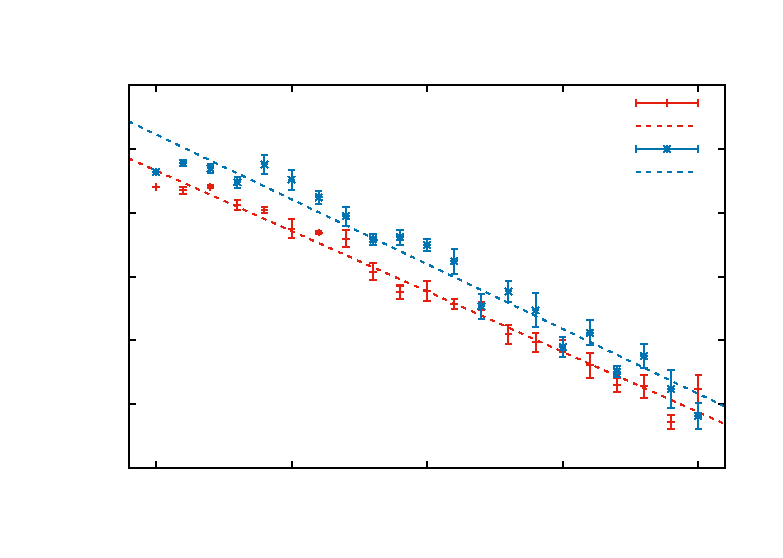
\includegraphics{figs/noise_1}}%
    \gplfronttext
  \end{picture}%
\endgroup
}}

\subfloat[\emph{Full GMHMM}]{\resizebox{\linewidth}{!}{% GNUPLOT: LaTeX picture with Postscript
\begingroup
  \makeatletter
  \providecommand\color[2][]{%
    \GenericError{(gnuplot) \space\space\space\@spaces}{%
      Package color not loaded in conjunction with
      terminal option `colourtext'%
    }{See the gnuplot documentation for explanation.%
    }{Either use 'blacktext' in gnuplot or load the package
      color.sty in LaTeX.}%
    \renewcommand\color[2][]{}%
  }%
  \providecommand\includegraphics[2][]{%
    \GenericError{(gnuplot) \space\space\space\@spaces}{%
      Package graphicx or graphics not loaded%
    }{See the gnuplot documentation for explanation.%
    }{The gnuplot epslatex terminal needs graphicx.sty or graphics.sty.}%
    \renewcommand\includegraphics[2][]{}%
  }%
  \providecommand\rotatebox[2]{#2}%
  \@ifundefined{ifGPcolor}{%
    \newif\ifGPcolor
    \GPcolortrue
  }{}%
  \@ifundefined{ifGPblacktext}{%
    \newif\ifGPblacktext
    \GPblacktextfalse
  }{}%
  % define a \g@addto@macro without @ in the name:
  \let\gplgaddtomacro\g@addto@macro
  % define empty templates for all commands taking text:
  \gdef\gplbacktext{}%
  \gdef\gplfronttext{}%
  \makeatother
  \ifGPblacktext
    % no textcolor at all
    \def\colorrgb#1{}%
    \def\colorgray#1{}%
  \else
    % gray or color?
    \ifGPcolor
      \def\colorrgb#1{\color[rgb]{#1}}%
      \def\colorgray#1{\color[gray]{#1}}%
      \expandafter\def\csname LTw\endcsname{\color{white}}%
      \expandafter\def\csname LTb\endcsname{\color{black}}%
      \expandafter\def\csname LTa\endcsname{\color{black}}%
      \expandafter\def\csname LT0\endcsname{\color[rgb]{1,0,0}}%
      \expandafter\def\csname LT1\endcsname{\color[rgb]{0,1,0}}%
      \expandafter\def\csname LT2\endcsname{\color[rgb]{0,0,1}}%
      \expandafter\def\csname LT3\endcsname{\color[rgb]{1,0,1}}%
      \expandafter\def\csname LT4\endcsname{\color[rgb]{0,1,1}}%
      \expandafter\def\csname LT5\endcsname{\color[rgb]{1,1,0}}%
      \expandafter\def\csname LT6\endcsname{\color[rgb]{0,0,0}}%
      \expandafter\def\csname LT7\endcsname{\color[rgb]{1,0.3,0}}%
      \expandafter\def\csname LT8\endcsname{\color[rgb]{0.5,0.5,0.5}}%
    \else
      % gray
      \def\colorrgb#1{\color{black}}%
      \def\colorgray#1{\color[gray]{#1}}%
      \expandafter\def\csname LTw\endcsname{\color{white}}%
      \expandafter\def\csname LTb\endcsname{\color{black}}%
      \expandafter\def\csname LTa\endcsname{\color{black}}%
      \expandafter\def\csname LT0\endcsname{\color{black}}%
      \expandafter\def\csname LT1\endcsname{\color{black}}%
      \expandafter\def\csname LT2\endcsname{\color{black}}%
      \expandafter\def\csname LT3\endcsname{\color{black}}%
      \expandafter\def\csname LT4\endcsname{\color{black}}%
      \expandafter\def\csname LT5\endcsname{\color{black}}%
      \expandafter\def\csname LT6\endcsname{\color{black}}%
      \expandafter\def\csname LT7\endcsname{\color{black}}%
      \expandafter\def\csname LT8\endcsname{\color{black}}%
    \fi
  \fi
    \setlength{\unitlength}{0.0500bp}%
    \ifx\gptboxheight\undefined%
      \newlength{\gptboxheight}%
      \newlength{\gptboxwidth}%
      \newsavebox{\gptboxtext}%
    \fi%
    \setlength{\fboxrule}{0.5pt}%
    \setlength{\fboxsep}{1pt}%
\begin{picture}(7200.00,5040.00)%
    \gplgaddtomacro\gplbacktext{%
      \csname LTb\endcsname%
      \put(946,704){\makebox(0,0)[r]{\strut{}0.65}}%
      \put(946,1439){\makebox(0,0)[r]{\strut{}0.7}}%
      \put(946,2174){\makebox(0,0)[r]{\strut{}0.75}}%
      \put(946,2909){\makebox(0,0)[r]{\strut{}0.8}}%
      \put(946,3644){\makebox(0,0)[r]{\strut{}0.85}}%
      \put(946,4379){\makebox(0,0)[r]{\strut{}0.9}}%
      \put(1338,484){\makebox(0,0){\strut{}0}}%
      \put(2639,484){\makebox(0,0){\strut{}0.5}}%
      \put(3941,484){\makebox(0,0){\strut{}1}}%
      \put(5242,484){\makebox(0,0){\strut{}1.5}}%
      \put(6543,484){\makebox(0,0){\strut{}2}}%
      \put(1338,1439){\makebox(0,0)[l]{\strut{}\footnotesize gmhmm: $y=-0.100x + 0.864$}}%
      \put(1338,1219){\makebox(0,0)[l]{\strut{}\footnotesize multiplex: $y=-0.100x + 0.869$}}%
    }%
    \gplgaddtomacro\gplfronttext{%
      \csname LTb\endcsname%
      \put(176,2541){\rotatebox{-270}{\makebox(0,0){\strut{}Accuracy}}}%
      \put(3940,154){\makebox(0,0){\strut{}Noise standard deviation, $\sigma_n$}}%
      \put(3940,4709){\makebox(0,0){\strut{}\bf Full GMHMM: Noise testing results}}%
      \csname LTb\endcsname%
      \put(5816,4206){\makebox(0,0)[r]{\strut{}\footnotesize gmhmm}}%
      \csname LTb\endcsname%
      \put(5816,3986){\makebox(0,0)[r]{\strut{}\footnotesize linear fit ($R^2 = 0.981$)}}%
      \csname LTb\endcsname%
      \put(5816,3766){\makebox(0,0)[r]{\strut{}\footnotesize multiplex}}%
      \csname LTb\endcsname%
      \put(5816,3546){\makebox(0,0)[r]{\strut{}\footnotesize linear fit ($R^2 = 0.989$)}}%
    }%
    \gplbacktext
    \put(0,0){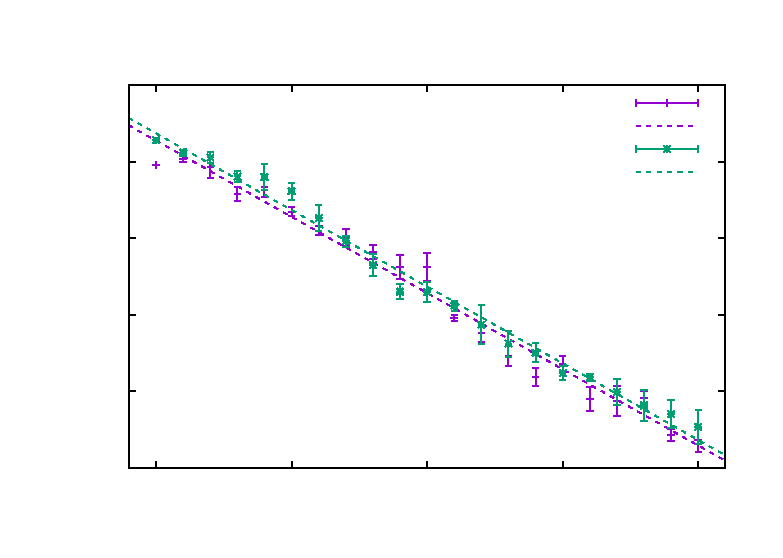
\includegraphics{figs/noise_2}}%
    \gplfronttext
  \end{picture}%
\endgroup
}}
\caption[Results of noise testing on the chain GMHMM models]{\centering Results of noise testing on the implemented models; error bars represent the standard error of the sample mean.}\label{fignoise1}
\end{figure}
%\begin{figure}[H]\centering
%\resizebox{0.9\linewidth}{!}{% GNUPLOT: LaTeX picture with Postscript
\begingroup
  \makeatletter
  \providecommand\color[2][]{%
    \GenericError{(gnuplot) \space\space\space\@spaces}{%
      Package color not loaded in conjunction with
      terminal option `colourtext'%
    }{See the gnuplot documentation for explanation.%
    }{Either use 'blacktext' in gnuplot or load the package
      color.sty in LaTeX.}%
    \renewcommand\color[2][]{}%
  }%
  \providecommand\includegraphics[2][]{%
    \GenericError{(gnuplot) \space\space\space\@spaces}{%
      Package graphicx or graphics not loaded%
    }{See the gnuplot documentation for explanation.%
    }{The gnuplot epslatex terminal needs graphicx.sty or graphics.sty.}%
    \renewcommand\includegraphics[2][]{}%
  }%
  \providecommand\rotatebox[2]{#2}%
  \@ifundefined{ifGPcolor}{%
    \newif\ifGPcolor
    \GPcolortrue
  }{}%
  \@ifundefined{ifGPblacktext}{%
    \newif\ifGPblacktext
    \GPblacktextfalse
  }{}%
  % define a \g@addto@macro without @ in the name:
  \let\gplgaddtomacro\g@addto@macro
  % define empty templates for all commands taking text:
  \gdef\gplbacktext{}%
  \gdef\gplfronttext{}%
  \makeatother
  \ifGPblacktext
    % no textcolor at all
    \def\colorrgb#1{}%
    \def\colorgray#1{}%
  \else
    % gray or color?
    \ifGPcolor
      \def\colorrgb#1{\color[rgb]{#1}}%
      \def\colorgray#1{\color[gray]{#1}}%
      \expandafter\def\csname LTw\endcsname{\color{white}}%
      \expandafter\def\csname LTb\endcsname{\color{black}}%
      \expandafter\def\csname LTa\endcsname{\color{black}}%
      \expandafter\def\csname LT0\endcsname{\color[rgb]{1,0,0}}%
      \expandafter\def\csname LT1\endcsname{\color[rgb]{0,1,0}}%
      \expandafter\def\csname LT2\endcsname{\color[rgb]{0,0,1}}%
      \expandafter\def\csname LT3\endcsname{\color[rgb]{1,0,1}}%
      \expandafter\def\csname LT4\endcsname{\color[rgb]{0,1,1}}%
      \expandafter\def\csname LT5\endcsname{\color[rgb]{1,1,0}}%
      \expandafter\def\csname LT6\endcsname{\color[rgb]{0,0,0}}%
      \expandafter\def\csname LT7\endcsname{\color[rgb]{1,0.3,0}}%
      \expandafter\def\csname LT8\endcsname{\color[rgb]{0.5,0.5,0.5}}%
    \else
      % gray
      \def\colorrgb#1{\color{black}}%
      \def\colorgray#1{\color[gray]{#1}}%
      \expandafter\def\csname LTw\endcsname{\color{white}}%
      \expandafter\def\csname LTb\endcsname{\color{black}}%
      \expandafter\def\csname LTa\endcsname{\color{black}}%
      \expandafter\def\csname LT0\endcsname{\color{black}}%
      \expandafter\def\csname LT1\endcsname{\color{black}}%
      \expandafter\def\csname LT2\endcsname{\color{black}}%
      \expandafter\def\csname LT3\endcsname{\color{black}}%
      \expandafter\def\csname LT4\endcsname{\color{black}}%
      \expandafter\def\csname LT5\endcsname{\color{black}}%
      \expandafter\def\csname LT6\endcsname{\color{black}}%
      \expandafter\def\csname LT7\endcsname{\color{black}}%
      \expandafter\def\csname LT8\endcsname{\color{black}}%
    \fi
  \fi
    \setlength{\unitlength}{0.0500bp}%
    \ifx\gptboxheight\undefined%
      \newlength{\gptboxheight}%
      \newlength{\gptboxwidth}%
      \newsavebox{\gptboxtext}%
    \fi%
    \setlength{\fboxrule}{0.5pt}%
    \setlength{\fboxsep}{1pt}%
\begin{picture}(7200.00,5040.00)%
    \gplgaddtomacro\gplbacktext{%
      \csname LTb\endcsname%
      \put(946,704){\makebox(0,0)[r]{\strut{}0.65}}%
      \put(946,1439){\makebox(0,0)[r]{\strut{}0.7}}%
      \put(946,2174){\makebox(0,0)[r]{\strut{}0.75}}%
      \put(946,2909){\makebox(0,0)[r]{\strut{}0.8}}%
      \put(946,3644){\makebox(0,0)[r]{\strut{}0.85}}%
      \put(946,4379){\makebox(0,0)[r]{\strut{}0.9}}%
      \put(1338,484){\makebox(0,0){\strut{}0}}%
      \put(2639,484){\makebox(0,0){\strut{}0.5}}%
      \put(3941,484){\makebox(0,0){\strut{}1}}%
      \put(5242,484){\makebox(0,0){\strut{}1.5}}%
      \put(6543,484){\makebox(0,0){\strut{}2}}%
      \put(1338,1439){\makebox(0,0)[l]{\strut{}\footnotesize gmhmm: $y=-0.100x + 0.864$}}%
      \put(1338,1219){\makebox(0,0)[l]{\strut{}\footnotesize multiplex: $y=-0.100x + 0.869$}}%
    }%
    \gplgaddtomacro\gplfronttext{%
      \csname LTb\endcsname%
      \put(176,2541){\rotatebox{-270}{\makebox(0,0){\strut{}Accuracy}}}%
      \put(3940,154){\makebox(0,0){\strut{}Noise standard deviation, $\sigma_n$}}%
      \put(3940,4709){\makebox(0,0){\strut{}\bf Full GMHMM: Noise testing results}}%
      \csname LTb\endcsname%
      \put(5816,4206){\makebox(0,0)[r]{\strut{}\footnotesize gmhmm}}%
      \csname LTb\endcsname%
      \put(5816,3986){\makebox(0,0)[r]{\strut{}\footnotesize linear fit ($R^2 = 0.981$)}}%
      \csname LTb\endcsname%
      \put(5816,3766){\makebox(0,0)[r]{\strut{}\footnotesize multiplex}}%
      \csname LTb\endcsname%
      \put(5816,3546){\makebox(0,0)[r]{\strut{}\footnotesize linear fit ($R^2 = 0.989$)}}%
    }%
    \gplbacktext
    \put(0,0){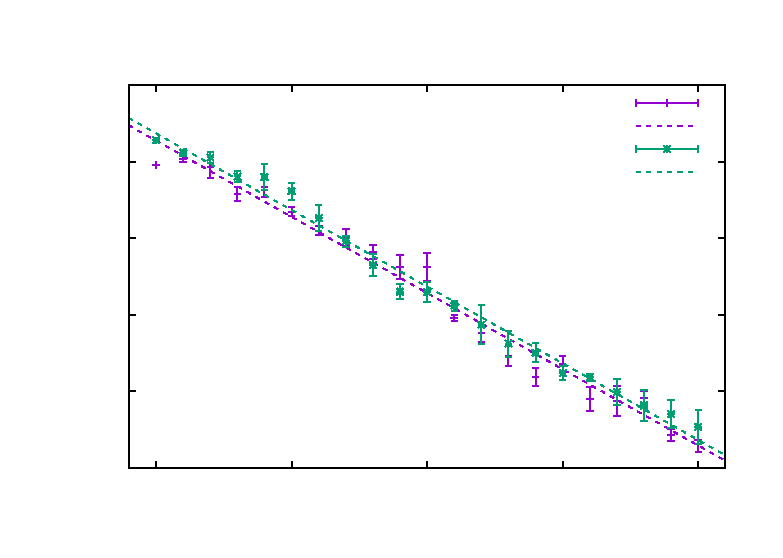
\includegraphics{figs/noise_2}}%
    \gplfronttext
  \end{picture}%
\endgroup
}
%\caption[Results of noise testing on the full GMHMM models]{\centering Results of noise testing on the full GMHMM models; error bars represent the standard error of the sample mean.}\label{fignoise2}
%\end{figure}
These results successfully demonstrate that the classification accuracy of the four implemented models decreases \emph{linearly} with the increase in the noise standard deviation, and as such, they demonstrate a {\bf good level of robustness to noise}. Furthermore, the comparative linear fits demonstrate that introducing multiplexity into the single-layer models does not cause any dramatic changes in robustness (the slopes of the linear fits remaining around $-0.1$).

\section{Summary}

In this chapter, I have provided a review of the methods used to verify that the project has met its success criteria, and the actual results obtained by those methods. This involved a brief overview of the adopted unit testing strategy, followed by a presentation of the obtained comparative evaluation and robustness analysis results.

\chapter{Conclusions}

\emph{Within this dissertation I have provided a thorough documentation of the preparatory, implementation and evaluation work I have performed while developing my project.\\ \\
This section will contain a few concluding remarks: a final summary of what has been achieved, the lessons I have learnt after successfully executing a project of this scale, and an overview of potential further extensions to the project.}

\section{Results}

As discussed in the previous chapters, \textbf{the project has met and exceeded all of its success criteria}, producing all of the expected core implementation deliverables along with several extensions.\!\! The models and their multiplex counterparts have both shown impressive performance and robustness when faced with a biomolecular classification problem on real data sets, and I have also demonstrated that introducing multiplexity results in more powerful classifiers without sacrificing robustness.\\ \\
Complex networks are currently a very active area of research; however, thus far little attention has been given to their utilisation in machine learning problems. I'm hopeful that the successes of my project---especially given that, to the best of my knowledge, there are no freely available implementations of multiplex networks in machine learning contexts---will provide a stepping-stone for me to partake in actively researching this application, as well as complex networks in general.

\section{Lessons learnt}

While not a research project by nature, my project involved combining known models and algorithms in a previously completely \emph{unexplored} context. This brought with it a great amount of risk, and a number of moments when there was no `prescribed' way of integrating the implemented components. Successfully overcoming issues like those required hours of research into ways that similar problems have been previously solved, and adapting the methods to be suitable within the context of my implementation.\\ \\
To me, this represented a very suitable introduction to methods of conducting research, and should be an important foundational skill for further study.

\section{Further work}

Although the project has been successful in achieving its success criteria, during development I have managed to identify several aspects where the implementation could be refined; these are summarised below.%\\ \\
%It is my intention to continue the development of the project, and eventually release the entire codebase as open-source. I anticipate that this will be helpful to researchers in the area of complex networks, as there are, to the best of my knowledge, no freely available implementations of multiplex networks in machine learning contexts.
\begin{itemize}
	\item \emph{Most-likely sequences of states}. The Baum-Welch algorithm produces a network where the states do not necessarily have any known meaning attached to them. Perhaps a way into researching these meanings would be to apply the Viterbi algorithm (Appendix \ref{secviterbi}) to the models and analyse the obtained state sequences; this would likely require collaboration with experts in the relevant fields.
	\item \emph{Optimising the NSGA-II parameters}. The parameters I have utilised for the genetic algorithm are the same as suggested in Deb \emph{et al.} \cite{deb2002fast}; the authors of the paper have explicitly stated that they have made no effort to optimise these parameters. While I am very satisfied with the performance shown by my model currently, it would be a viable effort to investigate how these parameters could be optimised, in order to obtain better quality solutions, higher rates of convergence, etc.
	\item \emph{Parallelisation}. Several components within the model implementation as well as the evaluation suite are \emph{`embarrassingly parallelisable'}, meaning that entire routines could easily be placed in separate threads to speed up the execution. Simple examples of this are the individual sequence trainings within the Baum-Welch algorithm and the crossover routine within NSGA-II. I am hoping to do a more thorough investigation of this and produce a model that executes faster through the use of concurrency.
\end{itemize}

%TC:ignore

%%%%%%%%%%%%%%%%%%%%%%%%%%%%%%%%%%%%%%%%%%%%%%%%%%%%%%%%%%%%%%%%%%%%%
% the bibliography
%\addcontentsline{toc}{chapter}{Bibliography}
\bibliography{refs}

%%%%%%%%%%%%%%%%%%%%%%%%%%%%%%%%%%%%%%%%%%%%%%%%%%%%%%%%%%%%%%%%%%%%%
% the appendices
\appendix

\chapter{Further theory}

\section{Introduction to hidden Markov models}\label{secintrohmm}

\subsection{Markov chains}

One simple way of defining a (discrete-state, discrete-time\footnote{It is possible to extend the definitions to the continuous case \cite{norris1998markov}, however this is outside the scope of my project, and is omitted.}) hidden Markov model is by augmenting its simpler variant, the \textbf{Markov chain} \cite{markov1906rasprostranenie}. Both of these models are stochastic models that satisfy the \textbf{Markov property} (\emph{memorylessness}):
\begin{mydef}\label{def:4}
\rm Let $S$ be a countable set of \emph{states}, and $\left\{X_n\right\}_{n \geq 0}$ a sequence of discrete random variables taking values $\left\{x_n\right\}_{n \geq 0}$ s.t. $\forall n\geq 0.\ x_n \in S$. This sequence satisfies the \emph{Markov property} if
\[\forall n\geq 1.\ \Prob(X_n = x_n | X_{n-1} = x_{n-1}, \dots, X_0 = x_0) = \Prob(X_n = x_n | X_{n-1} = x_{n-1})\]
and it is then called a \emph{Markov chain}.
\end{mydef}
\noindent Definition \ref{def:4} specifies that the probability distribution of the next state a Markov chain will have is determined solely by its current state. Furthermore it is often assumed that this distribution doesn't change over time (\textbf{time-homogeneity}):
\begin{mydef}
\rm A Markov chain $\left\{X_n\right\}_{n \geq 0}$ is \emph{time-homogeneous} if
\[\forall n\geq 1.\ \forall x, y \in S.\ \Prob(X_n = y | X_{n-1} = x) = \Prob(X_1 = y | X_0 = x)\]
\end{mydef}
\noindent Assuming time-homogeneity is convenient for representing Markov chains; if we also assume that the state set $S$ is finite, to fully specify the dynamics of any time-homogeneous Markov chain it is sufficient to specify:
\begin{itemize}
	\item A \textbf{start-state probability vector}\footnote{The start-state probability vector may be omitted if the start state is known in advance.}, $\vec{\pi}$, defined such that $\pi_x \myeq \Prob(X_0 = x)$;
	\item A \textbf{transition matrix}, ${\bf T}$, defined such that ${\bf T}_{xy} \myeq \Prob(X_1 = y | X_0 = x)$.
\end{itemize}
The probability of observing any particular state sequence $\{x_t\}_{t=0}^{T}$ then amounts to \[\Prob(\{x_t\}_{t=0}^{T}) = \Prob(X_0 = x_0)\prod\limits_{t=1}^{T}{\Prob(X_t = x_t|X_{t-1} = x_{t-1})} = \pi_{x_0}\prod\limits_{t=0}^{T-1}{{\bf T}_{x_t x_{t+1}}}\] In addition, such a Markov chain can be simply represented as a probabilistic finite state machine (refer to Figure \ref{figmarkchn}).
\begin{figure}
\centering
	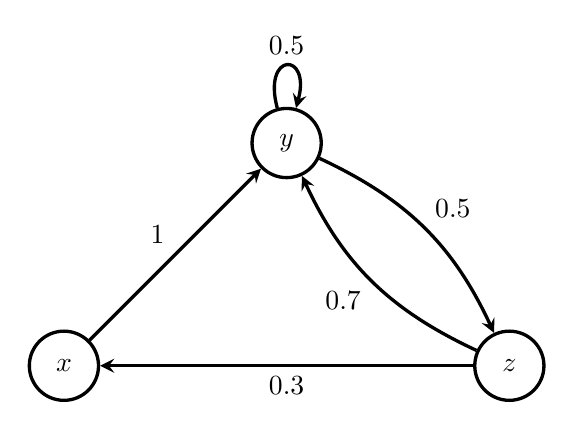
\begin{tikzpicture}[-stealth,very thick,node distance = 4cm,auto]

    \node[state] (x) {$x$};
    \node[state] (y) [above right of=x] {$y$};
    \node[state] (z) [below right of=y] {$z$};

	\draw[] (x) to node[above left] {$1$} (y);
	\draw[loop above] (y) to node {$0.5$} (y);
	\draw[bend left=20] (y) to node {$0.5$} (z);
	\draw[bend left=20] (z) to node[below left] {$0.7$} (y);
	\draw[] (z) to node {$0.3$} (x);

    %\path[-stealth, very thick]
    %(y) edge [bend right=20] node [left]{0.3} (x)
    %      edge [bend right=20] node {0.3} (z)
    %      edge [loop above, -stealth] node {0.4} ()
    %(x) edge [bend right=20] node {0.2} (y)
    %      edge [bend right=20] node {0.2} (z)
    %      edge [-stealth, loop left] node {0.6} ()
    %(z) edge [bend right=20] node [right]{0.1} (y)
    %      edge [bend right=20] node {0.1} (x)
    %      edge [-stealth, loop right] node {0.8} ();
  \end{tikzpicture}
\caption[Example of a time-homogeneous Markov chain]{Example of a time-homogeneous Markov chain with the state set $S = \{x, y, z\}$.}
\label{figmarkchn}
\end{figure}

\subsection{Hidden Markov models}

A hidden Markov model can now be built from the Markov chain, by means of the following definition:
\begin{mydef}
\rm	A \emph{hidden Markov model} (HMM) is a Markov chain in which the state sequence may be unobservable (\emph{hidden}).
\end{mydef}
\noindent This means that, while the Markov chain parameters (e.g. transition matrix and start-state probabilities in the time-homogeneous case) are still known, there is no way to determine the state sequence $\{X_n\}_{n\geq 0}$ the system will follow. What can be observed is the \textbf{output} sequence produced, $\{Y_n\}_{n\geq 0}$. The output sequence can assume any value from a given \textbf{set of outputs}, $O$. It is assumed that the output at any given moment \textbf{depends only on the current state}:
\[\forall n \geq 0.\ \Prob(Y_n = y_n | X_n = x_n,\dots,X_0 = x_0, Y_{n-1} = y_{n-1},\dots,Y_0 = y_0) = \Prob(Y_n = y_n | X_n = x_n)\]
If we furthermore assume that the set of outputs is finite, and that the output probability distribution doesn't change with time, i.e. \[\forall n \geq 0.\ \Prob(Y_n = y_n | X_n = x_n) = \Prob(Y_0 = y_n | X_0 = x_n)\]
then the only additional parameter we need to fully specify an HMM is the \textbf{output probability matrix}, ${\bf O}$, defined by ${\bf O}_{xy} \myeq \Prob(Y_0 = y | X_0 = x)$.\\ \\
An example of an HMM (extended from the Markov chain example) is given in Figure \ref{fighmmb}.

\begin{figure}
\centering
	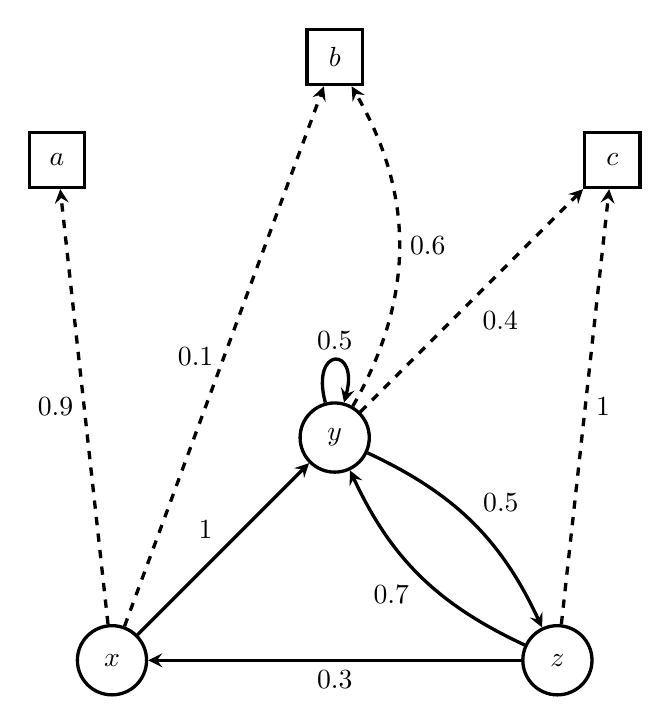
\begin{tikzpicture}[-stealth,very thick,node distance = 4cm,auto]

    \node[state] (x) {$x$};
    \node[state] (y) [above right of=x] {$y$};
    \node[state] (z) [below right of=y] {$z$};
    
    \node[rectangle, minimum size=2em,draw] (a) [above left =of y] {$a$};
    \node[rectangle,minimum size=2em, draw] (b) [above = of y] {$b$};
    \node[rectangle, minimum size=2em,draw] (c) [above right =of y] {$c$};

	\draw[] (x) to node[above left] {$1$} (y);
	\draw[loop above] (y) to node {$0.5$} (y);
	\draw[bend left=20] (y) to node {$0.5$} (z);
	\draw[bend left=20] (z) to node[below left] {$0.7$} (y);
	\draw[] (z) to node {$0.3$} (x);
	
	\draw[dashed] (x) to node[left] {$0.9$} (a);
	\draw[dashed] (x) to node[left] {$0.1$} (b);
	\draw[bend right=30, dashed] (y) to node[right] {$0.6$} (b);
	\draw[dashed] (y) to node[below right] {$0.4$} (c);
	\draw[dashed] (z) to node[right] {$1$} (c);

    %\path[-stealth, very thick]
    %(y) edge [bend right=20] node [left]{0.3} (x)
    %      edge [bend right=20] node {0.3} (z)
    %      edge [loop above, -stealth] node {0.4} ()
    %(x) edge [bend right=20] node {0.2} (y)
    %      edge [bend right=20] node {0.2} (z)
    %      edge [-stealth, loop left] node {0.6} ()
    %(z) edge [bend right=20] node [right]{0.1} (y)
    %      edge [bend right=20] node {0.1} (x)
    %      edge [-stealth, loop right] node {0.8} ();
  \end{tikzpicture}
\caption[Example of a hidden Markov model]{\centering Example of a hidden Markov model, extended from the Markov chain given in Figure \ref{figmarkchn} with the set of outputs $O=\{a, b, c\}$.}
\label{fighmmb}
\end{figure}

\subsection{Learning and inference}\label{seclrninfer}

As previously mentioned, an HMM is capable of solving a variety of machine learning problems; the fundamental three problems (as given in \cite{ferguson1980hidden}) are summarised here. To denote the HMM model parameters when describing the problems, the notation \linebreak${\bf \Theta} \myeq (\vec{\pi}, {\bf T}, {\bf O})$ will be used.
\begin{itemize}
	\item \emph{Probability of an observed output sequence.} Given an output sequence, $\{y_t\}_{t=0}^{T}$, determine the probability that it was produced by the given HMM ${\bf \Theta}$, i.e. \begin{equation}\Prob(Y_0 = y_0,\dots,Y_T = y_T | {\bf \Theta})\end{equation}
		This problem is efficiently solved with the \textbf{forward algorithm} (\cref{secfwdalgs}).
	\item \emph{Most likely sequence of states for an observed output sequence.} Given an output sequence, $\{y_t\}_{t=0}^{T}$, determine the most likely sequence of states, $\{\widehat{x}_t\}_{t=0}^{T}$, that produced it within a given HMM ${\bf \Theta}$, i.e. \begin{equation}\{\widehat{x}_t\}_{t=0}^{T} \myeq \argmax_{\{x_t\}_{t=0}^{T}}{\ \Prob(\{x_t\}_{t=0}^{T}|\{y_t\}_{t=0}^{T}, {\bf \Theta})}\end{equation}
		This problem is efficiently solved with the \textbf{Viterbi algorithm} \cite{viterbi1967error} (Appendix \ref{secviterbi}\footnote{The Viterbi algorithm is not used within my project, however I am describing it within an appendix because it could reasonably be applied in future work.}).
	\item \emph{Adjusting the model parameters.} Given an output sequence, $\{y_t\}_{t=0}^{T}$ and an HMM ${\bf \Theta}$, produce a new HMM ${\bf \Theta'}$ that is more likely to produce that sequence, i.e. \begin{equation}\Prob(\{y_t\}_{t=0}^{T}|{\bf \Theta'}) \geq \Prob(\{y_t\}_{t=0}^{T}|{\bf \Theta})\end{equation}
		This problem is efficiently solved with the \textbf{Baum-Welch Algorithm} (\cref{secbaumwelch}).
\end{itemize}

%\section{Multiplex network representation}\label{secmuxnetrep}

%Having formally defined multiplex networks, within this appendix I will provide a theoretical overview of a suggested mathematical structure for representing them\footnote{Other structures and generalisations are also available---refer to \cite{kivela2014multilayer}.}. Similarly as before, we may define a representation by generalising a structure we used for monoplex networks. \\ \\
%A commonly used structure for graph representation is the \emph{adjacency matrix}, ${\bf A}$, which is, for an unweighted graph $G = (V, E)$, defined such that 
%\[{\bf A}_{xy} \myeq \begin{cases}1 & (x, y) \in E\\ 0 & (x, y) \notin E\end{cases}\]
%Representing a graph in this way is often convenient, because e.g.\! it is then possible to apply various matrix algorithms on the adjacency matrix to compute features of the graph. Extending to multilayer networks as defined, this forces us to consider a four-dimensional space (pairs of node-layer pairs), corresponding to a {\bf rank-4 adjacency tensor}, $\mathcal{A}$. It is defined in a manner similar to the adjacency matrix:
%\[\mathcal{A}_{xy\alpha\beta} \myeq \begin{cases} 1 & ((x, G_\alpha), (y, G_\beta)) \in E_M\\0 & ((x, G_\alpha), (y, G_\beta)) \notin E_M \end{cases}\]
%There is a caveat with this representation, however; it {\bf requires} the multilayer network to be \emph{node-aligned} (as otherwise the pair $(x, G_\alpha)$ need not be in $V_M$). This is often alleviated by ``padding'' the layers with dummy nodes that are not incident on any edge (\cite{mucha2010communities, mucha2010community} as examples); however, the subsequent computation results must be interpreted with caution, as addition of dummy nodes can interfere with the correctness of even some of the more basic network metrics---a simple example of this is the degree of the network (defined as the average degree over all nodes). As more nodes of degree zero are added to the network, the average degree consistently drops.\\ \\
%As the network gets constrained, it might be possible to losslessly decrease the rank of $\mathcal{A}$. For \textbf{multiplex networks}, the constraint of \emph{diagonal coupling} is introduced; in that case, we know that $\mathcal{A}_{xy\alpha\beta} = 0$ for $x \neq y \wedge \alpha \neq \beta$. Hence it is sufficient to maintain \emph{two rank-3 tensors}, namely the {\bf intra-layer adjacency tensor}, $\mathcal{A}'$, defined as
%\[
%	\mathcal{A}_{xy\alpha}' \myeq \mathcal{A}_{xy\alpha\alpha}
%\]
%and the {\bf coupling tensor}, $\mathcal{C}$, defined as
%\[
%	\mathcal{C}_{x\alpha\beta} \myeq \mathcal{A}_{xx\alpha\beta}
%\]
%Furthermore, if the network is \emph{layer-coupled}, this allows us to reduce the dimensionality of the coupling tensor even further (as the coupling edge weights are then dependent only on the layer-pair involved); it would, in that case, be replaced with a rank-2 tensor, $\mathcal{C}'$ defined as follows:
%\[
%	\mathcal{C}_{\alpha\beta}' \myeq \mathcal{C}_{x\alpha\beta}\ (x \in V)
%\]
%Finally, if a special kind of coupling is used (e.g. categorical) and the network is unweighted, then the coupling tensor can be dropped altogether, and the network is fully represented by the intra-layer adjacency tensor.

\section{Viterbi algorithm}\label{secviterbi}

This appendix will contain a brief description of the Viterbi algorithm \cite{viterbi1967error}, which aims to find the most likely state sequence that produced a given output sequence $\vec{y}$ in a given HMM ${\bf\Theta} = (\vec{\pi}, {\bf T}, {\bf O})$.\\ \\
The algorithm employs a standard dynamic programming approach, computing the overall likelihood of ending up in state $x$ after processing the first $t$ elements of the output, $V_t(x)$. The base cases, $V_1(x)$, are simply calculated as
\[V_1(x) = \vec{\pi}_x{\bf O}_{x, y_1}\]
corresponding to starting in state $x$ and producing the first output from it. After computing all $V_t(x)$ values for some $t$, computing $V_{t+1}(x)$ may proceed as follows:
\[V_{t+1}(x) = \max_{x'\in S}{V_t(x'){\bf T}_{x'x}{\bf O}_{x, y_{t+1}}}\]
corresponding to ending up in $x'$ in the previous point in time, transitioning from $x'$ to $x$, and then producing the $(t+1)$-st output from it. It is also useful to store which state $x'$ has optimised the likelihood:
\[Ptr_{t+1}(x) = \argmax_{x'\in S}{V_t(x'){\bf T}_{x'x}{\bf O}_{x, y_{t+1}}}\]
The optimal state sequence $\vec{x}^*$, is then computed by backtracking; the final state $x_T^*$ is simply the one which maximises the overall likelihood, i.e.
\[x_T^* = \argmax_{x\in S} V_T(x)\]
and further states may be obtained using the relation
\[x_t^* = Ptr_{t+1}(x_{t+1}^*)\]
As with the majority of the algorithms discussed within this dissertation, the Viterbi algorithm is also prone to underflow problems; luckily, as all computations involved are multiplications, it is possible to trivially take the logarithm, and work only with sums of logarithms while computing the entries of $V_t(x)$.

\section{Simulated binary crossover/polynomial mutation}\label{secsbx}
Within this appendix, I will state the formulae for the simulated binary crossover \emph{(SBX)} operator, to produce two children real numbers $p'$ and $q'$ from parents $p$ and $q$. Furthermore, I will provide the formulae for the polynomial mutation operator, to mutate a given real number $x$, producing a new real number $x'$.\\ \\
The SBX operator has been defined in \cite{deb1994simulated}, and attempts to simulate the single-point crossover operator for binary strings; choosing a single point in the string after which the strings' contents are swapped to produce the children. Two parameters need to be specified: a real number $u\in [0, 1]$ drawn uniformly at random, and a parameter $\eta_c$ (used to control the spread of the produced solutions). First, define $\beta$ as follows:
\[\beta \myeq \begin{cases}
 (2u)^{\frac{1}{\eta_c + 1}} & u \leq 0.5\\
 \left(\frac{1}{2(1-u)}\right)^{\frac{1}{\eta_c + 1}} & \text{otherwise}	
 \end{cases}
\]
Then the produced children are:
\[p' = 0.5((1 + \beta)p + (1 - \beta)q)\]
\[q' = 0.5((1 - \beta)p + (1 + \beta)q)\]
Polynomial mutation attempts to introduce a variation in the value present; it does so by sampling a polynomial distribution. Similarly as before, a real number $u\in [0, 1]$ drawn uniformly at random is needed, as well as a spread-controlling parameter $\eta_m$. Define $\delta$ as follows:
\[\delta \myeq \begin{cases}
 (2u)^{\frac{1}{\eta_m + 1}} - 1 & u \leq 0.5\\
 1 - \left(2(1-u)\right)^{\frac{1}{\eta_m + 1}} & \text{otherwise}	
 \end{cases}
\]
Then the mutated value is:
\[x' = x + (x_{hi} - x_{lo})\delta\]
where $x_{lo}$ and $x_{hi}$ are the lower and upper bounds on $x$, respectively (constrained by the problem to be solved).

\chapter{Code samples}\label{seccodesamples}

This appendix contains select portions of the \CC\ code contained within my project's codebase, mainly for the purpose of illustrating some of the algorithms presented in the Implementation chapter.

\section{NSGA-II}
\subsection{Fast nondominated sort}

\begin{lstlisting}[numbersep=10pt]
vector<vector<chromosome> > NSGAII::fast_nondominated_sort(vector<chromosome> &P)
{
	vector<vector<chromosome> > F;
    
	vector<vector<int> > Sp;
	vector<int> np, Q;
	Sp.resize(P.size());
	np.resize(P.size());
	for (uint i=0;i<P.size();i++)
	{
		chromosome p = P[i];
		Sp[i].clear();
		np[i] = 0;
		for (uint j=0;j<P.size();j++)
		{
			chromosome q = P[j];
			if (dominated_by(p, q)) Sp[i].push_back(j);
			else if (dominated_by(q, p)) np[i]++;
		}
		if (np[i] == 0) Q.push_back(i);
	}
   
	vector<chromosome> Fi;
	Fi.resize(Q.size());
	for (uint i=0;i<Q.size();i++)
	{
		Fi[i] = P[Q[i]];
		Fi[i].rank = 1;
	}
	F.push_back(Fi);
    
	int ii = 1;
	while (!Q.empty())
	{
		vector<int> R;
		for (uint i=0;i<Q.size();i++)
		{
			for (uint j=0;j<Sp[Q[i]].size();j++)
			{
				int q = Sp[Q[i]][j];
				if (--np[q] == 0) R.push_back(q);
			}
		}
		ii++;
		if (R.empty()) break;
        
		Fi.resize(R.size());
		for (uint i=0;i<R.size();i++)
		{
			Fi[i] = P[R[i]];
			Fi[i].rank = ii;
		}
		F.push_back(Fi);
		Q = R;
	}
    
	P.clear();
	return F;
}
\end{lstlisting}

\subsection{Crowding distance assignment}

\begin{lstlisting}[numbersep=10pt]
void NSGAII::crowding_distance_assignment(vector<chromosome> &I)
{
	int l = I.size();
	for (int i=0;i<l;i++) I[i].distance = 0;
	for (int obj=0;obj<obj_size;obj++)
	{
		for (int i=0;i<l;i++) I[i].sort_key = obj;
		sort(I.begin(), I.end(), cmp_by_key);
		I[0].distance = I[l-1].distance = INF;
		for (int i=1;i<l-1;i++)
		{
			I[i].distance += I[i+1].values[obj] - I[i-1].values[obj];
		}
	}
}
\end{lstlisting}

\subsection{Solution combining}

\begin{lstlisting}[numbersep=10pt]
void NSGAII::make_new_pop(vector<chromosome> &P)
{
	for (int i=0;i<pop_size >> 1;i++)
	{
		chromosome p1, p2;
		p1 = P[select(P)];
		p2 = P[select(P)];
		pair<chromosome, chromosome> Cret = crossover(p1, p2);
		P.push_back(Cret.first);
		P.push_back(Cret.second);
	}
	mutate(P); // mutates only new generation, leaves first N alone
	for (int i=0;i<pop_size;i++)
	{
		for (int obj=0;obj<obj_size;obj++)
		{
			P[pop_size + i].values[obj] = objectives[obj](P[pop_size + i].features);
		}
	}
}
\end{lstlisting}

\subsection{Full iteration}

\begin{lstlisting}[numbersep=10pt]
void NSGAII::iterate()
{
	make_new_pop(main_population);
	vector<vector<chromosome> > fronts = fast_nondominated_sort(main_population);
	int ii = 0;
	while (main_population.size() + fronts[ii].size() <= uint(pop_size))
	{
		crowding_distance_assignment(fronts[ii]);
		main_population.insert(main_population.end(), fronts[ii].begin(), fronts[ii].end());
		ii++;
	}
	int elements_needed = pop_size - main_population.size();
	if (elements_needed > 0)
	{
		crowding_distance_assignment(fronts[ii]);
		sort(fronts[ii].begin(), fronts[ii].end());
		main_population.insert(main_population.end(), fronts[ii].begin(), fronts[ii].begin() + elements_needed);
	}
}
\end{lstlisting}

\section{GMHMM}
\subsection{Forward algorithm}

\begin{lstlisting}[numbersep=10pt]
tuple<double**, double*, double> GMHMM::forward(vector<pair<double, int> > &Y)
{
	int Ti = Y.size();
    
	double **alpha = new double*[Ti];
	for (int i=0;i<Ti;i++)
	{
		alpha[i] = new double[n];
	}
	double *c = new double[Ti];
    
	double sum = 0.0;
	for (int i=0;i<n;i++)
	{
		alpha[0][i] = pi[i] * O[i][Y[0].second] * get_probability(Y[0].second, Y[0].first);
		sum += alpha[0][i];
	}
	c[0] = 1.0 / sum;
	for (int i=0;i<n;i++)
	{
		alpha[0][i] /= sum;
	}
    
	for (int t=1;t<Ti;t++)
	{
		sum = 0.0;
		for (int i=0;i<n;i++)
		{
			alpha[t][i] = 0.0;
			for (int j=0;j<n;j++)
			{
				alpha[t][i] += alpha[t-1][j] * T[j][i];
			}
			alpha[t][i] *= O[i][Y[t].second] * get_probability(Y[t].second, Y[t].first);
			sum += alpha[t][i];
		}
        
		c[t] = 1.0 / sum;
		for (int i=0;i<n;i++)
		{
			alpha[t][i] /= sum;
		}
	}
    
	double log_L = 0.0;
	for (int i=0;i<Ti;i++) log_L -= log(c[i]);
    
	return make_tuple(alpha, c, log_L);
}
\end{lstlisting}

\subsection{Baum-Welch algorithm}

\begin{lstlisting}[numbersep=10pt]
void GMHMM::baumwelch(vector<vector<double> > &Ys, int iterations, double tolerance)
{
	vector<vector<pair<double, int> > > sorted_Ys;
	sorted_Ys.resize(Ys.size());
    
	for (uint l=0;l<Ys.size();l++)
	{
		sorted_Ys[l].resize(Ys[l].size());
		for (uint i=0;i<Ys[l].size();i++) sorted_Ys[l][i] = make_pair(Ys[l][i], i);
		sort(sorted_Ys[l].begin(), sorted_Ys[l].end());
	}
    
	double ***alpha = new double**[sorted_Ys.size()];
	double ***beta = new double**[sorted_Ys.size()];
	double **c = new double*[sorted_Ys.size()];
    
	double PP, QQ;
    
	double lhood = 0.0;
	double oldlhood = 0.0;
    
	for (int iter=0;iter<iterations;iter++)
	{
		lhood = 0.0;
        
		for (uint l=0;l<sorted_Ys.size();l++)
		{
			tuple<double**, double*, double> x = forward(sorted_Ys[l]);
			alpha[l] = get<0>(x);
			c[l] = get<1>(x);
			lhood += get<2>(x);
			beta[l] = backward(sorted_Ys[l], c[l]);
		}
        
		double **nextO = new double*[n];
		for (int i=0;i<n;i++) nextO[i] = new double[obs];
        
		for (int i=0;i<n;i++)
		{
			pi[i] = 0.0;
			for (uint l=0;l<sorted_Ys.size();l++)
			{
				pi[i] += alpha[l][0][i] * beta[l][0][i];
			}
			pi[i] /= sorted_Ys.size();
            
			QQ = 0.0;
            
			for (int k=0;k<obs;k++)
			{
				nextO[i][k] = 0.0;
			}
            
			for (uint l=0;l<sorted_Ys.size();l++)
			{
				for (uint t=0;t<sorted_Ys[l].size()-1;t++)
				{
					double curr = alpha[l][t][i] * beta[l][t][i];
					QQ += curr;
					nextO[i][sorted_Ys[l][t].second] += curr;
				}
			}
            
			for (int j=0;j<n;j++)
			{
				PP = 0.0;
				for (uint l=0;l<sorted_Ys.size();l++)
				{
					for (uint t=0;t<sorted_Ys[l].size()-1;t++)
					{
						PP += alpha[l][t][i] * O[j][sorted_Ys[l][t+1].second] * get_probability(sorted_Ys[l][t+1].second, sorted_Ys[l][t+1].first) * beta[l][t+1][j] * c[l][t+1];
					}
				}
				T[i][j] *= PP / QQ;
			}
            
			for (uint l=0;l<sorted_Ys.size();l++)
			{
				int lim = sorted_Ys[l].size() - 1;
				double curr = alpha[l][lim][i] * beta[l][lim][i];
				QQ += curr;
				nextO[i][sorted_Ys[l][lim].second] += curr;
			}
            
			for (int k=0;k<obs;k++)
			{
				nextO[i][k] /= QQ;
			}
		}
        
		for (uint l=0;l<sorted_Ys.size();l++)
		{
			for (uint t=0;t<sorted_Ys[l].size();t++)
			{
				delete[] alpha[l][t];
				delete[] beta[l][t];
			}
			delete[] alpha[l];
			delete[] beta[l];
			delete[] c[l];
		}
        
		for (int i=0;i<n;i++)
		{
			delete[] O[i];
		}
		delete[] O;
        
		O = nextO;
        
		if (fabs(lhood - oldlhood) < tolerance) break;
		oldlhood = lhood;
	}
}	
\end{lstlisting}

\subsection{Multiplex training}

\begin{lstlisting}[numbersep=10pt]
void MultiplexGMHMM::train(vector<vector<vector<double> > > &train_set)
{
	// Train all the layers individually (as before)
	for (int l=0;l<L;l++)
	{
		vector<vector<double> > curr_set(train_set.size(), vector<double>(obs));
		for (uint i=0;i<train_set.size();i++)
		{
			for (int j=0;j<obs;j++)
			{
				curr_set[i][j] = train_set[i][j][l];
			}
		}
		layers[l] -> train(curr_set);
	}
    
	// Run the algorithm
	NSGAII nsga2;
	vector<chromosome> candidates = nsga2.optimise(params, objectives);
    
	// Evaluate the best choice of omega
	int best = -1;
	double min_sum = -1.0;
	for (uint i=0;i<candidates.size();i++)
	{
		sort(candidates[i].values.begin(), candidates[i].values.end());
		double curr_sum = 0.0;
		for (uint j=0;j<train_set.size();j++)
		{
			curr_sum += (j + 1) * candidates[i].values[j];
		}
		if (best == -1 || curr_sum < min_sum)
		{
			best = i;
			min_sum = curr_sum;
		}
	}
    
	// Adjust the parameters accordingly
	double **fin_omega = new double*[L];
	for (int i=0;i<L;i++)
	{
		fin_omega[i] = new double[L];
		for (int j=0;j<L;j++)
		{
			fin_omega[i][j] = candidates[best].features[i*L + j];
		}
	}
    
	set_omega(fin_omega);
    
	for (int i=0;i<L;i++) delete[] fin_omega[i];
	delete[] fin_omega;
}
\end{lstlisting}

\chapter{Unit tests}\label{secapptests}

This appendix contains a direct reference to the unit tests used to verify correctness of the principal algorithms within my project. \\ \\
It should be noted that the HMM algorithms have been tested on an HMM with \emph{discrete} outputs, due to the greater abundance of such examples available. This is sufficient, due to the fact that extending them to the GMHMM case only requires multiplying by an additional value (the PDF of a Gaussian distribution).

\section{Forward/backward algorithm}

This test case is based on the ``umbrella world'', given in Russell \& Norvig \cite{Russell:2003:AIM:773294}.\\ \\
The parameters of the HMM are:
\[n = m = 2\]
\[{\vec{\pi}} = \left(\begin{matrix}
 0.5 & 0.5\\	
 \end{matrix}\right)
\]
\[{\bf T} = \left(\begin{matrix}
 0.7 & 0.3\\
 0.3 & 0.7\\	
 \end{matrix}\right)
\]
\[{\bf O} = \left(\begin{matrix}
 0.9 & 0.1\\
 0.2 & 0.8\\	
 \end{matrix}\right)
\]
The observed output sequence is:
\[\vec{y} = \left(\begin{matrix}
 0 & 0 & 1 & 0 & 0\\	
 \end{matrix}\right)
\]
The expected (normalised) forward and backward likelihoods after each step are:
\[
\hat{\alpha} = \left(\begin{matrix}
	0.8182 & 0.8834 & 0.1907 & 0.7308 & 0.8673\\
	0.1818 & 0.1166 & 0.8093 & 0.2692 & 0.1327\\
\end{matrix}\right)
\]
\[
\hat{\beta} = \left(\begin{matrix}
	0.5923 & 0.3763 & 0.6533 & 0.6273 & 0.5000\\
	0.4077 & 0.6237 & 0.3467 & 0.3727 & 0.5000\\
\end{matrix}\right)
\]
\newpage
\section{Baum-Welch algorithm}

This test case is based on the ``Finding Keyser S\"{o}ze'' worked example given in a lecture by E. Frazzoli \cite{FrazzoliMIT}.\\ \\
The initial HMM parameters are:
\[n = 2, m = 3\]
\[{\vec{\pi}} = \left(\begin{matrix}
 0.5 & 0.5\\	
 \end{matrix}\right)
\]
\[{\bf T} = \left(\begin{matrix}
 0.5 & 0.5\\
 0.5 & 0.5\\	
 \end{matrix}\right)
\]
\[{\bf O} = \left(\begin{matrix}
 0.4 & 0.1 & 0.5\\
 0.1 & 0.5 & 0.4\\	
 \end{matrix}\right)
\]
The observed output sequence is:
\[\vec{y} = \left(\begin{array}{cccccccccccccccccccc}
 2 & 0 & 0 & 2 & 1 & 2 & 1 & 1 & 1 & 2 & 1 & 1 & 1 & 1 & 1 & 2 & 2 & 0 & 0 & 1\\	
 \end{array}\right)
\]
After convergence, the following parameters of the HMM are expected\footnote{As termination criteria may be different, the final output is accepted if it is within $\varepsilon=10^{-3}$ of the expected parameters.}:
\[{\vec{\pi}'} = \left(\begin{matrix}
 1 & 0\\	
 \end{matrix}\right)
\]
\[{\bf T'} = \left(\begin{matrix}
 0.6909 & 0.3091\\
 0.0934 & 0.9066\\	
 \end{matrix}\right)
\]
\[{\bf O'} = \left(\begin{matrix}
 0.5807 & 0.0010 & 0.4183\\
 0.0000 & 0.7621 & 0.2379\\	
 \end{matrix}\right)
\]

\section{NSGA-II}

The test cases used are the same as the ones used in Deb \emph{et al.} \cite{deb2002fast} to evaluate NSGA-II, and are outlined in Table \ref{tblnsgatest}.

\begin{table}
\hspace*{-1.05cm}\begin{tabular}{ l c c l c l } \toprule
{\bf Test} & {$\bf{n}$} & {\bf Constraints} & {\bf Objectives (to \underline{minimise})} & {\bf Optimal front}\\ \midrule
SCH & $1$ & $x \in [-10^3, 10^3]$ & $f_1(x) = x^2$ & $x\in [0, 2]$ &\\
& & & $f_2(x) =(x-2)^2$ &\\
& & & & &\\
FON & $3$ & $x_i \in [-4, 4]$ & $f_1(\vec{x}) = 1 - \exp{\left(-\sum_{i=1}^3 {\left(x_i - \frac{1}{\sqrt{3}}\right)^2}\right)}$ & $x_1 = x_2 = x_3$\\
 &  &  & $f_2(\vec{x}) = 1 - \exp{\left(-\sum_{i=1}^3 {\left(x_i + \frac{1}{\sqrt{3}}\right)^2}\right)}$ & $\in [-\frac{1}{\sqrt{3}}, \frac{1}{\sqrt{3}}]$\\
 & & & & &\\
POL & $2$ & $x_i \in [-\pi, \pi]$ & $f_1(\vec{x}) = 1 + (A_1 - B_1)^2 + (A_2 - B_2)^2$ & ref. \cite{deb2001multi} \\
 & & & $f_2(\vec{x}) = (x_1+3)^2 + (x_2+1)^2$ &\\
 & & & $A_1 = 0.5\sin{1} - 2\cos{1} + \sin{2} - 1.5\cos{2}$ &\\
 & & & $A_2 = 1.5\sin{1} - \cos{1} + 2\sin{2} - 0.5\cos{2}$ &\\
 & & & $B_1 = 0.5\sin{x_1} - 2\cos{x_1} + \sin{x_2} - 1.5\cos{x_2}$ &\\
 & & & $B_2 = 1.5\sin{x_1} - \cos{x_1} + 2\sin{x_2} - 0.5\cos{x_2}$ &\\
 & & & & &\\
KUR & $3$ & $x_i \in [-5, 5]$ & $f_1(\vec{x}) = \sum_{i=1}^{n-1}{-10\exp{\left(-0.2\sqrt{x_i^2 + x_{i+1}^2}\right)}}$ & ref. \cite{deb2001multi} \\
 & & & $f_2(\vec{x}) = \sum_{i=1}^{n}{|x_i|^{0.8} + 5\sin{x_i^3}}$ &\\
 & & & & &\\
ZDT1 & $30$ & $x_i \in [0, 1]$ & $f_1(\vec{x}) = x_1$ & $x_1\in [0, 1]$\\
 & & & $f_2(\vec{x}) = g(\vec{x})\left(1-\sqrt{\frac{x_1}{g(\vec{x})}}\right)$ & $x_i = 0$\\
 & & & $g(\vec{x}) = 1 + 9\frac{\sum_{i=2}^n {x_i}}{n-1}$ & $(i \neq 1)$\\
 & & & & &\\
ZDT2 & $30$ & $x_i \in [0, 1]$ & $f_1(\vec{x}) = x_1$ & $x_1\in [0, 1]$\\
 & & & $f_2(\vec{x}) = g(\vec{x})\left(1-\left(\frac{x_1}{g(\vec{x})}\right)^2\right)$ & $x_i = 0$\\
 & & & $g(\vec{x}) = 1 + 9\frac{\sum_{i=2}^n {x_i}}{n-1}$ & $(i \neq 1)$\\
 & & & & &\\
ZDT3 & $30$ & $x_i \in [0, 1]$ & $f_1(\vec{x}) = x_1$ & $x_1\in [0, 1]$\\
 & & & $f_2(\vec{x}) = g(\vec{x})\left(1-\sqrt{\frac{x_1}{g(\vec{x})}} - \frac{x_1}{g(\vec{x})}\sin{(10\pi x_1)}\right)$ & $x_i = 0$\\
 & & & $g(\vec{x}) = 1 + 9\frac{\sum_{i=2}^n {x_i}}{n-1}$ & $(i \neq 1)$\\
 & & & & &\\
ZDT4 & $10$ & $x_1 \in [0, 1]$ & $f_1(\vec{x}) = x_1$ & $x_1\in [0, 1]$\\
 & & $x_i \in [-5, 5]$ & $f_2(\vec{x}) = g(\vec{x})\left(1-\sqrt{\frac{x_1}{g(\vec{x})}}\right)$ & $x_i = 0$\\
 & & $(i \neq 1)$ & $g(\vec{x}) = 1 + 10(n-1) + \sum_{i=2}^n {x_i^2 - 10\cos{(4\pi x_i)}}$ & $(i \neq 1)$\\
 & & & & &\\
ZDT6 & $10$ & $x_i \in [0, 1]$ & $f_1(\vec{x}) = x_1$ & $x_1\in [0, 1]$\\
 & & & $f_2(\vec{x}) = g(\vec{x})\left(1-\left(\frac{f_1(\vec{x})}{g(\vec{x})}\right)^2\right)$ & $x_i = 0$\\
 & & & $g(\vec{x}) = 1 + 9\left(\frac{\sum_{i=2}^n {x_i}}{n-1}\right)^{0.25}$ & $(i \neq 1)$\\
\bottomrule
\end{tabular}
\caption[A summary of the unit tests on NSGA-II]{A summary of the unit tests on NSGA-II.}\label{tblnsgatest}
\end{table}

\chapter{Project Proposal}\label{secprop}

\documentclass[12pt,a4]{article}
\usepackage[margin=1.3in]{geometry}
\usepackage[UKenglish]{isodate}
\usepackage[colorlinks=true, linkcolor=red, citecolor=green, filecolor=magenta, urlcolor=blue]{hyperref}
\usepackage[T1]{fontenc}
\usepackage{enumitem}
\usepackage{amsmath}
\cleanlookdateon


\begin{document}

\thispagestyle{empty}

\newcommand{\HRulee}{\rule{\linewidth}{0.5mm}}

\vfil

{\raggedleft \large Petar Veli\v{c}kovi\'{c} \\}
{\raggedleft \large Trinity College \\}
{\raggedleft \large \tt pv273 \\}

\vfil

\begin{center}

	{\Large \sc Project Proposal \\}
	\vspace{10pt}
	{\Large \sc Computer Science Tripos, Part II \\}
	\vspace{20pt}
	\HRulee \\[0.1cm]
	{\LARGE \bf Molecular multiplex network inference \\}
	\HRulee \\[20pt]
	{\Large 23 October 2014 \\}
	\vspace{20pt}
\end{center}

\vfil

\noindent\emph{\textbf{Project Originators:}}\\
	Dr Pietro Li\`{o}\\
	Petar Veli\v{c}kovi\'{c}\\

\vspace{10pt}
	
\noindent\emph{\textbf{Project Supervisor:}}\\
	Dr Pietro Li\`{o}\\

\vspace{10pt}
	
\noindent\emph{\textbf{Director of Studies:}}\\
	Dr Arthur C. Norman\\
	
\vspace{10pt}
	
\noindent\emph{\textbf{Project Overseers:}}\\
	Prof Peter Robinson\\
	Dr Robert N. Watson\\

% BLOCK VERSION	

%\begin{minipage}{0.4\textwidth}
%\begin{flushleft} \large
%\noindent\emph{\textbf{Project Originators:}}\\
%	Dr Pietro Li\`{o}\\
%	Petar Veli\v{c}kovi\'{c}\\
%\end{flushleft}
%\end{minipage}
%~
%\begin{minipage}{0.4\textwidth}
%\begin{flushright} \large
%\noindent\emph{\textbf{Project Supervisor:}}\\
%	Dr Pietro Li\`{o}\\
%\hfill \\
%\end{flushright}
%\end{minipage}\\
	
%\vspace{40pt}

%\begin{minipage}{0.4\textwidth}
%\begin{flushleft} \large
%\noindent\emph{\textbf{Director of Studies:}}\\
%	Dr Arthur C. Norman\\
%	\hfill \\
%\end{flushleft}
%\end{minipage}
%~
%\begin{minipage}{0.4\textwidth}
%\begin{flushright} \large
%\noindent\emph{\textbf{Project Overseers:}}\\
%	Prof Peter Robinson\\
%	Dr Robert N. Watson\\
%\end{flushright}
%\end{minipage}\\
	
\newpage
	
\section*{Introduction and Description of the Work}

Machine learning, and statistical analysis in general, are crucial methods in the development of the field of diagnostic medicine. Determining whether or not, for example, a patient is infected with a certain type of disease given the symptoms he is experiencing or laboratory results, can be ideally presented as a problem solved by a classifier. As another example, we may be interested in knowing whether the patient is at significant risk of developing a disease, or, if he/she already is affected, the likely prognosis of the development of the disease -- these may often be represented as regression problems. \\ \\
The importance of such models is greater than ever, now that various kinds of biomolecular data can be extracted with greater certainty. However, most current machine learning model implementations will tend to operate on a single type of data only. This can still provide us with precise inferences, however in reality most of the data types, particularly at the molecular level, exhibit a level of \emph{correlation} that is differently pronounced depending on the biological process/disease in question. It is therefore to be expected that taking into account several data types at once and modelling their interactions correctly within our machine learning model should provide us with even better inferences. These interactions are not fully understood, but are assumed to be more complicated than what simply combining two separate structures in a predictable way can model. As such, there is a need for creating a data structure which may be trained to learn from data sets of each individual type as well as to model their correlation. \\ \\
With this project I propose a possible solution to this problem -- combining multiple \emph{hidden Markov models} (HMMs) over identical sets of nodes, each of which has been individually trained on a single type of data, with additional interlayer links -- this kind of multilayered graph is known as a \emph{multiplex network}. To the best of my knowledge, there currently exists no open-source implementation of a structure like this. As multiple types of correlated data arise in a multitude of fields, it is expected that a generic implementation of this project will prove useful not only to bioinformaticians, but essentially anyone having to perform any kind of statistical analysis. The language of choice for the implementation of this project is C++, because I already have substantial experience in it, and it is optimised for performance -- hence, it can accommodate evaluation on larger data sets compared to the other options I had.

\section*{Starting Point}

The project implementation will draw material from the following courses of the Computer Science Tripos:

\paragraph{$\sim$ Bioinformatics} Being the central project area, this course provides an overview of biological contexts behind the machine learning models utilised, as well as examples of hidden Markov model usage in analysing biomolecular data;
\paragraph{$\sim$ Artificial Intelligence I/II} The material covered in these courses is closely related to the methods utilised in this project, such as machine learning and optimisation. In particular, the standard algorithms on hidden Markov models are covered within it.
\paragraph{$\sim$ Programming in C/C++} As previously mentioned, C++ will be the language of choice for the implementation of this project. I already have an extensive experience with the language, having used it primarily for competitive algorithmic programming. This course has provided me with an introduction to templates, which I will be using extensively to create as generic library elements as possible.\\ \\
The Bioinformatics course is ongoing as this proposal is being written, while I will need to familiarise myself with the relevant Artificial Intelligence II material in advance. Material relevant to other aspects of the project (primarily in the form of academic papers and open-source projects) will be investigated in the initial stages, as outlined in the timetable.

\section*{Substance and Structure of the Project}
As outlined in the introductory section, this project intends to produce a data structure for supervised machine learning (separate training and test data sets for purposes of classification and/or regression) which will accommodate for multiple types of data that are correlated in an undefined way with respect to the problem at hand. The key three building blocks of this data structure are as follows:
\begin{itemize}
    \item \textbf{Hidden Markov models} (HMMs) will be used to model the solution to the problem by utilising each individual data type provided. More precisely, the full data structure will consist of multiple HMMs over the same set of nodes (for example, these may represent genes or patients), each of which has been trained on a particular type of data.
    \item \textbf{Multiplex networks} are then used to intertwine these individual layers together. In the most general form, a multiplex network over $L$ layers and $n$ nodes can be represented as an $L \times L$ matrix of $n \times n$ matrices
    \[
        \bf M =
 \begin{pmatrix}
  {\bf A}_{11} & {\bf A}_{12} & \cdots & {\bf A}_{1L} \\
  {\bf A}_{21} & {\bf A}_{22} & \cdots & {\bf A}_{2L} \\
  \vdots  & \vdots  & \ddots & \vdots  \\
  {\bf A}_{L1} & {\bf A}_{L2} & \cdots & {\bf A}_{LL}
 \end{pmatrix}
    \]
    where ${\bf A}_{ii}$ corresponds to the edge weight matrix representing the $i$th individual layer, that is, $\left({\bf A}_{ii}\right)_{jk}$ represents the weight of the edge between nodes $j$ and $k$ in the $i$th layer. Similarly, ${{\bf A}_{xy}}\ (x \neq y)$ corresponds to the interlayer connections between layers $x$ and $y$. More precisely, $\left({\bf A}_{xy}\right)_{ij}$ represents the weight of the edge between node $i$ in layer $x$, and node $j$ in layer $y$. In practice, the interlayer connections are usually modelled in the form ${{\bf A}_{xy}} = \omega_{xy} \bf I$ (where $\bf I$ is the identity matrix), i.e. a node is only linked to its own image in the other layer, and all edges between a particular pair of layers have equal weight. \\ \\
    A multiplex network is a special case of \emph{multilayered graphs}, enforcing that all the layers are built over the same set of nodes. The solution to the problem of combining correlated data sets for machine learning may be pursued by considering construction of general multilayered graphs, however these fall out of the scope of the types of data used for evaluating this project.
    \item \textbf{Multiobjective genetic algorithms} are to be used in the final step of the construction of the data structure, which is training the multiplex -- that is, determining the interlayer connection matrices ${\bf A}_{xy}$ (usually just the coefficients $\omega_{xy}$, as discussed above) that will yield optimal inferences on the test set. These algorithms solve the \emph{multiobjective optimisation problem}, which may be formulated as minimising several functions $f_1(\vec{x}), f_2(\vec{x}), \dots, f_n(\vec{x})$ simultaneously. For the purposes of training the multiplex network, we would want to optimise the probabilities of each training set being properly classified by the model.
\end{itemize}
The execution of the project has been split into five main objectives. Their completion has been specifically marked within the milestones given in the project timetable below. The objectives are as follows, in chronological order:
\begin{itemize}
    \item \textbf{\textsc{Preparation}} -- this objective consists of preparatory background reading on the theory behind the data structures and algorithms given above. To confirm successful completion of this chapter as well as commence work on the full project, a working implementation of a hidden Markov model should be produced at the end of this phase and tested on data provided in the literature.
    \item \textbf{\textsc{Core project implementation}} -- this objective consists of implementing the main building blocks and integrating them in a full data structure with a classification inference algorithm. Most, if not all, tests will be executed with a two-layered multiplex, but the design should be in principle extendable to an arbitrary amount of layers.
    \item \textbf{\textsc{Core project evaluation}} -- this objective consists of evaluating the performance of the implementation mentioned above, both on small and large data sets. The evaluation will be performed in two main ways:
    \begin{itemize}
        \item \textbf{Supervised learning setup}: dividing the given data sets into \emph{training} and \emph{testing} subsets, constructing the implemented data structure using the training set and afterwards examining the quality of its predictions on the testing set, against the known classifications provided therewith;
        \item \textbf{Comparison with individual layers}: testing the gain we have made by combining different types of data. This involves constructing the individual HMM layers trained on the same data as the entire structure, using only one of the data types provided within the data sets, and then comparing the accuracy of those single-layer classifiers with the accuracy of the implemented data structure on the testing set.
    \end{itemize}
    The classification problem that will be addressed in the evaluation of this project is classifying patients for diabetes. The layers of the multiplex will be trained and tested on two related types of biomolecular data that have been correlated with the presence of diabetes: 
    \begin{itemize}
        \item \emph{DNA methylation} (amount of $\text{CH}_3$ (methyl-) groups attached to the base nucleotides in particular genes);
        \item \emph{Gene expression} (measure of the activity of transcription of particular genes into proteins).
    \end{itemize}
    \item \textbf{\textsc{Extensions}} -- this objective consists of augmenting the data structure with two additional functionalities identified as extensions: one of them is the addition of \emph{regression} inference algorithms (producing continuous output as opposed to the discrete output of the classifier), and the other is introduction of tunable \emph{"random noise"} in the structure (in the form of adding/removing nodes/edges, or modifying edge weights by a random amount), to accommodate for the slightly stochastic nature of these processes. Both extensions should be implemented and evaluated, time permitting, upon completion of the core project.
    \item \textbf{\textsc{Dissertation}} -- this objective consists of writing up the project dissertation, documenting how all of the above objectives have been achieved in a clear and logical order.
\end{itemize}

\section*{Success Criteria}

The project will be considered a success upon satisfactory completion of the \textbf{\textsc{Preparation}}, \textbf{\textsc{Core project implementation}}, \textbf{\textsc{Core project evaluation}} and \textbf{\textsc{Dissertation}} objectives as outlined above. Precisely:
\begin{itemize}
    \item The complete proposed classifier data structure should be implemented, incorporating at least the three main building blocks outlined in the previous section. Correct operation of the individual modules within the structure should be tested on the sample tests provided in relevant literature or academic papers.
    \item The accuracy of the classifier should be evaluated with at least the two methods given in the previous section (supervised learning setup to estimate accuracy, and comparison with single-layered classifiers). It might prove useful to provide further ways of evaluation, e.g. of the structure's running time/space efficiency on the training and testing sets; these methods should be investigated as needed.
    \item Finally, a dissertation should be produced, documenting the necessary introduction to the problem area, the work done in the stages of preparation, implementation and evaluation of the project, and the conclusions drawn from the project's overall execution.
\end{itemize}
 The \textbf{\textsc{Extensions}} objective should also be achievable, however it is orthogonal to the core project and as such is not essential to its success.

\section*{Resources Required}

I intend to use my own laptop (2.6 GHz Intel Core i7 with 8 GB RAM, running Mac OS X 10.10 Yosemite) for the purposes of implementation, evaluation and dissertation writeup. I accept full responsibility for this machine and I have made the following contingency plans to protect myself against hardware/software failures:

\begin{itemize}
    \item Revision control of the project's codebase and dissertation using \texttt{git}, with all commits pushed onto a remote private repository on GitHub (with intents of making it public upon completion of the project);
    \item Synchronisation of the entire project with my personal file spaces on Dropbox, Google Drive and the MCS utilising \texttt{rsync}, both manually and automatically;
    \item Regular backups of the machine's entire filesystem (and hence the project files as well) utilising Apple's Time Machine, on an external 1TB HDD.
\end{itemize}
For evaluation purposes, the project will also utilise molecular data (DNA methylation and gene expression matrices of patients, with provided classifications for diabetes) located in the Gene Expression Omnibus (\url{http://www.ncbi.nlm.nih.gov/geo/}). This data is readily available, and I am familiar with the methods of accessing the relevant sets. \\ \\
This project is not expected to rely on any libraries for the three major modules outlined in the project substance, as some proposed features such as adding random noise to the model and making the model generic may not be easily integrated with the current implementations available, justifying an implementation from scratch. However, in the event of a major schedule overrun, the project implementation may fall back to extending an existing library.

\section*{Timetable and Milestones}

To facilitate execution of the project in accordance with the proposed structure, I have divided the project development timetable into fifteen fortnightly slots, some of which have been reserved for initial research and dissertation writeup, and some serving as buffer time in the event of schedule overruns. To keep track of the progress of the project, I have assigned a milestone to each slot -- it should be verified at the end of each slot that its respective milestone has been achieved. \\ \\
The rough plan is to complete the core project by the end of December, implement proposed extensions by mid-February, and produce a final dissertation writeup ready for submission by late April. The full proposed timetable is given below:

\begin{enumerate}[label=\bf Slot \arabic*:]
    \setcounter{enumi}{-1}
    \item \emph{6 October -- 22 October}
        \begin{itemize}
            \item[$\rightarrow$] Working on the project proposal.
            \item[$\rightarrow$] Setup of all contingency schemes as described in the resource declaration section.
            \item[$\rightarrow$] Studying the essentials of hidden Markov models from relevant literature and the previous year's Artificial Intelligence II course notes.
        \end{itemize}
        \textbf{Milestone:} Project proposal ready for submission.
    \item \emph{23 October -- 5 November}\\
        \underline{\textbf{\textsc{Deadline:}}} Project proposal submission (24 October)
        \begin{itemize}
            \item[$\rightarrow$] Researching academic papers relevant to multiplex networks, and investigating genetic algorithm implementations and their relative merits.
            \item[$\rightarrow$] Starting work on a generic HMM implementation in C++.
        \end{itemize}
        \textbf{Milestone:} A basic working HMM implementation, tested on a few examples given in literature (\textbf{\textsc{Preparation completed}}).
    \item \emph{6 November -- 19 November}
        \begin{itemize}
            \item[$\rightarrow$] Implementation of a generic multiplex network class. 
            \item[$\rightarrow$] Integration of the HMM as a layer in the multiplex.
        \end{itemize}
        \textbf{Milestone:} Successfully connecting two HMMs in a multiplex network. Providing a front-end command line tool which can read and analyse a multiplex given in a prescribed format.
    \item \emph{20 November -- 3 December}
        \begin{itemize}
            \item[$\rightarrow$] Implementation of inference algorithms on multiplex networks; verification that the algorithms produce expected outputs on known networks.
        \end{itemize}
        \textbf{Milestone:} Inferences of comparable quality successfully made on known examples of multiplex networks (from research papers).
    \item \emph{4 December -- 17 December}
        \begin{itemize}
            \item[$\rightarrow$] Implementation of a suitable genetic algorithm to be used for training the interlayer edge weights for the multiplex network.
        \end{itemize}
        \textbf{Milestone:} Working generic implementation of the genetic algorithm, tested on example functions given in relevant academic papers.
    \item \emph{18 December -- 31 December}
        \begin{itemize}
            \item[$\rightarrow$] Integration of the genetic algorithm with what was previously done; utilising it to train the underlying multiplex as described.
            \item[$\rightarrow$] Attempting a first evaluation run on a small data set; fixing any residual bugs in the design as found.
        \end{itemize}
        \textbf{Milestone:} Classifier successfully ran on a small data set (\textbf{\textsc{Core project implementation completed}}).
    \item \emph{1 January -- 14 January}
        \begin{itemize}
            \item[$\rightarrow$] Evaluating the core project by training and testing on large data sets; in particular, performing a comparison with HMM classifiers over a single data type.

            \item[$\rightarrow$] Writing the progress report; if necessary, sending it to the supervisor and incorporating any comments. 
        \end{itemize}
        \textbf{Milestone:} Progress report ready for submission. Classifier performance evaluated on large data sets (\textbf{\textsc{Core project evaluation completed}}).
    \item \emph{15 January -- 28 January}
        \begin{itemize}
            \item[$\rightarrow$] Implementing a regression method of inference on the multiplex HMM structure. Running on the provided data sets, and commenting on the obtained results.
            \item[$\rightarrow$] Prepare slides for the progress report presentation (utilising output from the evaluation as needed).
        \end{itemize}
        \textbf{Milestone:} Successful regression performed on the multiplex, producing useful output for the given training and testing data sets. Presentation slides prepared. 
    \item \emph{29 January -- 11 February}\\
        \underline{\textbf{\textsc{Deadline:}}} Progress report submission (30 January)
        \begin{itemize}
            \item[$\rightarrow$] Rehearse and deliver presentation to overseeing group.
            \item[$\rightarrow$] Implementation of a feature to allow introducing random noise into the multiplex structure, either by adding extra nodes/edges or modifying the values of existing ones. Commenting on performance with respect to the noise parameter(s).
        \end{itemize}
        \textbf{Milestone:} Presentation successfully delivered. A working scheme for adding noise into the model, with appropriate testing conducted (\textbf{\textsc{Extensions completed}}).
    \item \emph{12 February -- 25 February}
        \begin{itemize}
            \item[$\rightarrow$] Buffer slot \#1, to accommodate any schedule overruns with the implementation; if there are none, start work on the dissertation early.
        \end{itemize}
        \textbf{Milestone:} None.
    \item \emph{26 February -- 11 March}
        \begin{itemize}
            \item[$\rightarrow$] Starting work on the dissertation; completion of preparatory chapters.
        \end{itemize}
        \textbf{Milestone:} Completion of the Introduction and Preparation chapters of the dissertation.
    \item \emph{12 March -- 25 March}
        \begin{itemize}
            \item[$\rightarrow$] Completion of draft dissertation.
            \item[$\rightarrow$] Submission of the draft to the supervisor and Director of Studies.
        \end{itemize}
        \textbf{Milestone:} Completion of the Implementation, Evaluation and Conclusion chapters of the dissertation. Submission of the first draft.
        \item \emph{26 March -- 8 April}
        \begin{itemize}
            \item[$\rightarrow$] Receipt of responses from the supervisor, Director of Studies and any proofreaders.
            \item[$\rightarrow$] Incorporation of the obtained comments as appropriate, in preparation of the second draft of the dissertation.
        \end{itemize}
        \textbf{Milestone:} Submission of the second draft of the dissertation to the supervisor and Director of Studies.
    \item \emph{9 April -- 22 April}
        \begin{itemize}
            \item[$\rightarrow$] Receipt of responses on the second draft.
            \item[$\rightarrow$] Incorporate any further comments as appropriate.
        \end{itemize}
        \textbf{Milestone:} Final version of the dissertation ready for submission.
    \item \emph{23 April -- 6 May}
        \begin{itemize}
            \item[$\rightarrow$] Print, bind and submit the dissertation.
        \end{itemize}
        \textbf{Milestone:} Submission of dissertation (\textbf{\textsc{Dissertation completed}}).
    \item \emph{7 May -- 13 May}
        \begin{itemize}
            \item[$\rightarrow$] Buffer slot \#2, to accommodate any unexpected issues with the writeup of the dissertation.
            \item[$\rightarrow$] Revision for Part II examinations.
        \end{itemize}
        \underline{\textbf{\textsc{Deadline:}}} Dissertation submission (15 May)
\end{enumerate}


\end{document}



%TC:endignore

\end{document}
